\documentclass[A4paper,11pt]{article}
\usepackage{amsmath,amssymb,amsfonts,amsthm}
\usepackage{enumerate}
%\usepackage{enumitem}
\usepackage{paralist}
\usepackage{graphics} %% add this and next lines if pictures should be in esp format
\usepackage{float}
\usepackage{epsfig} %For pictures: screened artwork should be set up with an 85 or 100 line screen
\usepackage{graphicx}
\usepackage{epstopdf}%This is to transfer .eps figure to .pdf figure; please compile your paper using PDFLeTex or PDFTeXify.
%\usepackage[colorlinks=true]{hyperref}
%\hypersetup{urlcolor=blue, citecolor=red}
\usepackage{hyperref}
%\usepackage{refcheck}

\usepackage{bm}
\usepackage{color}

%  \textheight=8.2 true in
%   \textwidth=5.0 true in
%    \topmargin 30pt
%     \setcounter{page}{1}

\usepackage[a4paper]{geometry}

\newtheorem{theorem}{Theorem}[section]
\newtheorem{corollary}[theorem]{Corollary}
\newtheorem*{main}{Main Theorem}
\newtheorem{lemma}[theorem]{Lemma}
\newtheorem{proposition}[theorem]{Proposition}
\newtheorem{conjecture}{Conjecture}
\newtheorem*{problem}{Problem}
\theoremstyle{definition}
\newtheorem{definition}[theorem]{Definition}
\newtheorem{remark}{Remark}
\newtheorem{example}{Example}
\newtheorem*{notation}{Notation}
\newtheorem{assumption}{Assumption}
\newcommand{\ep}{\varepsilon}
\newcommand{\eps}[1]{{#1}_{\varepsilon}}

\newcommand{\vnorm}[1]{\left\| #1 \right\|}
\newcommand{\scalarp}[1]{\left\langle #1 \right\rangle}
\newcommand{\redd}[1]{{\color{red}{#1}}}

\newcommand{\Lip}{\textup{Lip}}
\newcommand{\loc}{\textup{loc}}

\newcommand{\N}{\mathbb{N}}
\newcommand{\Z}{\mathbb{Z}}
\newcommand{\Q}{\mathbb{Q}}
\newcommand{\R}{\mathbb{R}}
\newcommand{\cb}{\mathcal{B}}
\newcommand{\cf}{\mathcal{F}}
\newcommand{\ch}{\mathcal{H}}
\newcommand{\cl}{\mathcal{L}}
\newcommand{\cn}{\mathcal{N}}
\newcommand{\ct}{\mathcal{T}}
\newcommand{\W}{\mathcal{W}}
\newcommand{\PP}{\mathcal{P}_1}
\newcommand{\PC}{\mathcal{P}_c}
\DeclareMathOperator{\supp}{supp}
\DeclareMathOperator{\sgn}{sgn}
\DeclareMathOperator{\diag}{diag}
\DeclareMathOperator{\diam}{diam}
\DeclareMathOperator{\argmin}{arg\,min}
\DeclareMathOperator{\Span}{span}
\DeclareMathOperator*{\esssup}{ess\,sup}

\newcommand{\Fun}[1]{F^{[#1]}}
\newcommand{\Energy}{\mathcal E}
\newcommand{\Ea}[1]{\Energy^{[a]}(#1)}
\newcommand{\Eahat}{\Ea{\widehat a}}
\newcommand{\Ean}{\Energy^{[a],N}}
\newcommand{\Eahatn}{\Ean(\widehat a)}
\newcommand{\prerho}{\overline\rho}
\newcommand{\x}{x^{[a]}}
\newcommand{\xahat}{x^{[\widehat a]}}
\newcommand{\dotx}{\dot{x}^{[a]}}
\newcommand{\dotxahat}{\dot{x}^{[\widehat a]}}


\newcommand{\MMcomment}[1]{{\color{blue}{#1}}}
\newcommand{\MFcomment}[1]{{\color{red}{#1}}}
\allowdisplaybreaks

\graphicspath{{Figures1/}}

\title{Inferring Interaction Rules from Observations of Evolutive Systems I: The Variational Approach}

\author{M. Bongini\footnote{Faculty of Mathematics, Technical University of Munich, Boltzmannstrasse 3, 85748 Garching bei M\"unchen, Germany, Email: mattia.bongini@ma.tum.de}, 
M. Fornasier\footnote{Faculty of Mathematics, Technical University of Munich, Boltzmannstrasse 3, 85748 Garching bei M\"unchen, Germany, Email: massimo.fornasier@ma.tum.de}, 
M. Hansen\footnote{Faculty of Mathematics, Technical University of Munich, Boltzmannstrasse 3, 85748 Garching bei M\"unchen, Germany, Email: markus.hansen@ma.tum.de}, 
and M. Maggioni\footnote{Department of Mathematics, Duke University, 	117 Physics Bldg., Science Dr., Box 90320
Durham, NC 27708-0320
U.S.A., Email: mauro@math.duke.edu}}

\date{}

\begin{document}
\maketitle

\begin{abstract}
In this paper we are concerned with the  learnability of nonlocal interaction kernels for  first order systems modeling certain social interactions, from observations of realizations of their dynamics. This paper is the first  of a series  on learnability of nonlocal interaction kernels and presents a variational approach to the problem. In particular, we assume here that  the kernel to be learned is bounded and locally Lipschitz continuous and that the initial conditions of the systems are drawn identically and independently at random according to a given initial probability distribution. Then the minimization over a rather arbitrary  sequence of (finite dimensional) subspaces of a least square functional measuring the discrepancy from observed trajectories  produces uniform approximations to the kernel on compact sets. The convergence result is obtained by combining mean-field limits, transport methods, and a $\Gamma$-convergence argument. A crucial condition for the learnability is a certain coercivity property of the least square functional, majoring an $L_2$-norm discrepancy to the kernel with respect to a probability measure, depending on the given initial probability distribution by suitable push forwards and transport maps. We illustrate the convergence result by means of several numerical experiments. 
\end{abstract}
{\bf Keywords}: nonlocal interaction kernel learning, first order nonlocal interaction equations, mean-field equations, $\Gamma$-convergence

\bigskip

\tableofcontents

% !TEX root = dynamicslearning.tex
\section{Introduction}

What are the instinctive individual reactions which make a group of animals forming coordinated movements, for instance a flock of migrating birds or a school of fish? Which biological interactions between cells produce the formation of complex structures, like tissues and organs? What are the mechanisms which induce certain significant changes in a large amount of players in the financial market? 
In this paper we are concerned with the ``mathematization'' of the problem of learning or inferring interaction rules from observations of evolutions. The framework we consider is the one of  evolutions driven by gradient descents.
The study of gradient flow evolutions to minimize  certain energetic landscapes has been the subject of intensive research in the past years \cite{AGS}. Some of the most recent models are  aiming at describing time-dependent phenomena also in biology or even in social dynamics, borrowing a leaf from more established and classical  models in physics. For instance, starting with the seminal papers of Vicsek et. al. \cite{VCBCS95} and Cucker-Smale \cite{CucSma07}, there has been a flood of models describing consensus or opinion formation,  modeling the exchange of information as long-range social interactions (forces) between active agents (particles). However, for the analysis, but even more crucially for the reliable and realistic numerical simulation of such phenomena, one presupposes a complete understanding and determination of the governing energies. Unfortunately, except for physical situations where the calibration of the model can be done by measuring the governing forces rather precisely, for some relevant macroscopical models in physics and most of the models in biology and social sciences the governing energies are far from being precisely determined. In fact, very often in these studies the governing energies are just predetermined to be able to reproduce, at least approximately or qualitatively, some of the macroscopical effects of the observed dynamics, such as the formation of certain patterns, but there has been relatively little effort in the applied mathematics literature towards matching data from real-life cases. 

%This attitude aiming just at a qualitative description tends however to reduce  some of the investigations in this area to  %beautiful and mathematically interesting toy-cases, which have likely little to do with real-life scenarios. 
In this paper we aim at bridging in the specific setting of first order models, the well-developed theory of dynamical systems and mean-field equations with classical  approaches of approximation theory, nonlinear time series analysis, and machine learning. We  provide a  mathematical framework for the reliable identification of the governing forces from data obtained by direct observations of corresponding time-dependent evolutions. This is a new kind of inverse problem, beyond more traditionally considered ones, as the forward map is a strongly nonlinear  evolution, highly dependent on the probability measure generating the initial conditions. As we aim at a precise quantitative analysis, and to be very concrete, we will  attack the learning of the governing laws of evolution for specific models in social dynamics governed by nonlocal interactions. The models considered in the scope of this paper are deterministic, however we intend in follow up work to extend our results towards stochastic dynamical systems.




% !TEX root = dynamicslearning.tex

\subsection{General abstract framework}

Many time-dependent phenomena in physics, biology, and social sciences can be modeled by a function $x:[0,T] \to \mathcal H$, where $\mathcal H$ represents the space of states of the physical, biological or social system, which evolves from an initial configuration $x(0)=x_0$  towards a more convenient state or a new equilibrium. The space $\mathcal H$ can be a conveniently chosen Banach space or just a metric space; let $\operatorname{dist}_{\mathcal H}$ be the metric on $\mathcal H$.
This implicitly assumes that $x$ evolves driven by a minimization process of a potential energy $\mathcal J: \mathcal H \times [0,T] \to \mathbb R$.  In this preliminary introduction we consciously avoid specific assumptions on  $\mathcal J$, as we wish to keep a rather general view. We restrict the presentation to particular cases below.%

Inspired by physics, for which conservative forces are the derivatives of the potential energies, one can describe the evolution as satisfying a gradient flow inclusion of the type
\begin{equation}\label{gradientflow}
\dot x(t) \in - \partial_x \mathcal J(x(t),t),
\end{equation}
where $\partial_x \mathcal J(x,t)$ is some notion of differential of $\mathcal J$ with respect to $x$, which might already take into consideration additional constraints which are binding the states to certain sets.



\subsection{Example of gradient flow of nonlocal particle interactions}\label{sec:gradflow}

Assume that $x=(x_1,\dots,x_N) \in \mathcal H= \mathbb R^{d\times N}$ and that 
$$
\mathcal J_N(x) = \frac{1}{2N} \sum_{i,j=1}^N A(| \x_i -  \x_j |),
$$
where $A:\mathbb R_+ \to \mathbb R$ is a suitable nonlinear interaction kernel function, which, for simplicity we assume to be smooth, and $|\cdot|$ is the Euclidean norm in $\mathbb R^d$. Then, the formal unconstrained gradient flow \eqref{gradientflow} associated to this energy is written coordinatewise as
\begin{equation}\label{fdgradientflow}
\dotx_i(t) = \frac{1}{N} \sum_{j \neq i} \frac{A'(| \x_i -  \x_j |)}{| \x_i -  \x_j |} (\x_j - \x_i), \quad i=1,\dots,N.
\end{equation}
Under suitable assumptions of local Lipschitz continuity and boundedness of 
\begin{equation}\label{intker}
a(\cdot) := \frac{A'(|\cdot|)}{| \cdot |},
\end{equation} this evolution is well-posed for any given $x(0)=x_0$ and it is expected to converge for $t \to \infty$ to configurations of the points whose mutual distances are close to local minimizers of the function $A$, representing steady states of the evolution as well as critical points of $\mathcal J_N$.\\
It is also well-known \cite{AGS} (see also Proposition \ref{pr:exist} below) that for $N \to \infty$ a mean-field approximation holds: if the initial conditions $\x_i(0)$ are i.i.d. according to a compactly supported probability measure $\mu^0 \in \mathcal P_c(\mathbb R^d)$ for $i=1,2,3, \dots$, the empirical measure $\mu_N(t) = \frac{1}{N} \sum_{i=1}^N \delta_{\x_i(t)}$ weakly converges for $N \to \infty$  to the probability measure-valued trajectory $t \to \mu(t)$ satisfying weakly the equation
\begin{equation}\label{eq:meanfield}
\partial_t \mu(t) = - \nabla \cdot ((\Fun{a} * \mu(t)) \mu(t)), \quad \mu(0)=\mu^0.
\end{equation}
where $\Fun{a}(z) =-a(|z|)z=-A'(|z|)$, for $z \in \mathbb R^{d}$. In fact the differential equation \eqref{eq:meanfield} corresponds again to a gradient flow of the ``energy''
$$
\mathcal J (\mu) = \int_{\mathbb R^{d\times d}} A(| x-  y |) d \mu(x) d\mu(y),
$$
on the metric space $\mathcal H =\mathcal P_c(\mathbb R^d)$ endowed with the so-called Wasserstein distance. Continuity equations of the type \eqref{eq:meanfield} with nonlocal interaction kernels are currently the subject of intensive research  towards the modeling of the biological and social behavior of microorganisms, animals, humans, etc. We refer to the  articles \cite{cafotove10,13-Carrillo-Choi-Hauray-MFL} for recent overviews on this subject. Despite the tremendous theoretical success of such research direction in terms of mathematical results, as we shall stress below in more detail, one of the issues which is so far scarcely addressed in the study of models of the type \eqref{fdgradientflow} or \eqref{eq:meanfield} is their actual applicability. Most of the results are addressing a purely {\it qualitative analysis} given certain smoothness and asymptotic properties of the kernels $A$ or $a$ at the origin or at infinity, in terms of well-posedness or in terms of asymptotic behavior of the solution for $t \to \infty$.  Certainly such results are of great importance, as such interaction functions, if ever they can really describe social dynamics,  are likely to differ significantly from well-known models from physics and it is reasonable and legitimate to consider a large variety of classes of such functions.
However, a solid mathematical framework which establishes the conditions of ``learnability'' of the interaction kernels from observations of the dynamics is currently not available and it will be the main subject of this paper.

\subsection{Parametric energies and their identifications}

Let us now consider an energy $\mathcal J[a]$ depending on a parameter function $a$. As in the example mentioned above, $a$ may be defining a nonlocal interaction kernel as in  \eqref{intker}. The parameter function $a$ not only determines the energy, but also the corresponding evolutions driven according to \eqref{gradientflow}, for fixed initial conditions $x(0)=x_0$. (Here we assume that the class of $a$ is such that the evolutions exist and they are essentially well-posed.)
The fundamental question to be addressed is: can we recover $a$ with high accuracy given some observations of the realized evolutions? This question is prone to several specifications, for instance, we may want to assume that the initial conditions are generated according to a certain probability distribution or they are chosen deterministically ad hoc to determine at best $a$, that the observations are complete or incomplete, etc. As one  quickly realizes, this is a very broad field to explore with many possible developments. Surprisingly, there are no results in this direction at this level of generality, and very little is done in the specific directions we mentioned in the example above. We refer for instance to \cite{mann11,heoemascszwa11} for studies on the inference of social rules in collective behavior. 
\subsection{The optimal control approach and its drawbacks}
Let us introduce an approach, which would perhaps naturally be considered at a first instance and focus for a moment on the gradient flow model \eqref{gradientflow}. Given a certain gradient flow evolution $t \to x[a](t)$ depending on the unknown parameter function $a$, one might decide to design the recovery of $a$ as an optimal control problem \cite{brpi07}: for instance, we may seek a parameter function $\widehat a$ which minimizes
\begin{equation}\label{optcontr}
\Eahat = \frac{1}{T}\int_0^T \left [ \operatorname{dist}_{\mathcal H}(\x(s) - \xahat(s))^2 + \mathcal R(\widehat a) \right ] d s ,
\end{equation}
being $t \to x[\widehat a](t)$ the solution of gradient flow \eqref{gradientflow} for $\mathcal J = \mathcal J[\widehat a]$, i.e.,
\begin{equation}\label{gradientflow2}
\dotxahat(t) \in - \partial_x J(x[\widehat a](t),t),
\end{equation}
and $\mathcal R(\cdot)$ is a suitable regularization function, which restricts the possible minimizers of \eqref{optcontr} to a specific class. The first fundamental problem one immediately encounters with this formulation is the strongly nonlinear dependency of $t \to \xahat(t)$ on $\widehat a$, which results in a strong non-convexity of the functional \eqref{optcontr}. This also implies that a direct minimization of \eqref{optcontr} would risk to lead to suboptimal solutions, and even the computation of a first order optimality condition in terms of Pontryagin's minimum principle would not characterize uniquely the minimal solutions. Besides this fundamental hurdles, the numerical implementation of either strategy (direct optimization or solution of the first order optimality conditions) is expected to be computationally unfeasible to reasonable degree of accuracy as soon as the underlying discretization dimension grows.

\subsection{A variational approach towards learning parameter functions in nonlocal energies}\label{sec:wp2}

Let us consider the framework of the example in Section \ref{sec:gradflow}. We restrict our attention to interaction kernels $a$ belonging to the following \textit{set of admissible kernels}
\begin{align*}
	X=\bigl\{b:\R_+\rightarrow\R\,|\ b \in L_{\infty}(\R_+) \cap W^{1}_{\infty,\loc}(\R_+) \bigr \}.
\end{align*}
In particular every $a \in X$ is weakly differentiable, and its local Lipschitz constant $\Lip_{K}(a)$ is finite for every compact set $K \subset \R_+$.
Our goal is to learn the unknown influence function $a \in X$ from the observation of the dynamics of the empirical measure $\mu_N$, defined by $\mu_N(t)=\frac{1}{N} \sum_{i=1}^N \delta_{\x_i(t)}$, where $\x a_i(t)$ are driven by the interaction kernel $a$ according to the equations of motion
\begin{equation}\label{fdgradientflow2}
\dotx_i(t) = \frac{1}{N} \sum_{j \neq i} a(| \x_i -  \x_j |) (\x_j - \x_i), \quad i=1,\dots,N.
\end{equation}
%We already mentioned that the most immediate approach of formulating the learning of $a$ in terms of an optimal control problem is not efficient and likely will not give optimal solutions due to the strong non-convexity. 
Instead of the nonlinear optimal control problem above, we propose an alternative, direct approach which is both computationally very efficient and produces accurate approximations under reasonable assumptions.
We consider a minimizer of the following \textit{discrete error functional}
\begin{align}\label{eq-def-error1}
	\begin{split}
	\Eahatn = \frac{1}{T}\int_0^T\frac{1}{N}\sum_{i=1}^N\biggl|\frac{1}{N}\sum_{j=1}^N
			\left(\widehat a(|\x_i(t)-\x_j(t)|)(\x_i(t) - \x_j(t))-\dotx_i(t)\right)\biggr|^2 dt,
	\end{split}
\end{align}
among all functions $\widehat a \in X$. 
The minimization of $\Eahatn$ has a close connection to the optimal control problem \eqref{optcontr}:
\begin{proposition}\label{trajapprox}
If $a,\widehat a \in X$ then there exist a constant $C>0$ depending on $T,\widehat a$ and $\mu_0^N$ and a compact set $K \subset \R_+$ such that
\begin{equation}\label{eq:trajapprox}
\| \x (t) -\xahat  (t) \|^2 \leq C {\Eahatn}, 
\end{equation}
for all $t \in [0,T]$, and $\x , \xahat  $ are the solutions to \eqref{eq:discrdyn} for the interaction kernels $a$ and $\widehat a$ respectively. (Here $\| x \| = \frac{1}{N} \sum_{i=1}^N |x_i|$ \MMcomment{$\| x \|^2 = \frac{1}{N} \sum_{i=1}^N |x_i|^2$?}, for $x \in \mathbb R^{d \times N}$.)
\end{proposition}


%In Proposition \ref{trajapprox} we show that if both $a, \widehat a \in X$ then there exist a constant $C>0$ depending on $T, \widehat a, \mu_N^0$ and a compact set $K \subset \R_+$ such that
%$$
%\| \xahat (t) -\x (t) \| \leq C (\|\widehat a\|_\infty + \operatorname{Lip}_K(\widehat a)) \sqrt{\Eahatn}, 
%$$
%for all $t \in [0,T]$. Here $\| x \| = \frac{1}{N} \sum_{i=1}^N |x_i|$ \MMcomment{isn't it: $\| x \|^2 := \frac{1}{N} \sum_{i=1}^N |x_i|^2$?}, for $x \in \mathbb R^{d \times N}$. 
Therefore if $\widehat a$ makes $\Eahatn$ small, the trajectories $t\to \xahat(t)$ of the system \eqref{fdgradientflow2} with interaction kernel $\widehat a$ instead of $a$ are an approximation of the trajectories $t \to \x(t)$ at finite time. 
Moreover, contrary to the optimal control approach, the functional $\Ean$ can be easily computed from witnessed trajectories $\x_i(t)$ and $\dotx_i(t)$. We may consider discrete-time approximations the time derivative $\dotx_i$ (e.g. by finite differences) and we shall assume that the data of the problem is the full set of observations $\x_i(t)$ for $t \in [0,T]$, for a prescribed finite time horizon $T>0$. Moreover, being a simple quadratic functional, its minimizers can be efficiently numerically approximated on a finite element space: given a finite dimensional space $V \subset X$, we let:
\begin{equation}\label{fdproxy}
\widehat a_{N,V} = \argmin_{\widehat a \in V} \Eahatn.
\end{equation}
The fundamental question to be addressed in this paper is
\begin{itemize}
\item[(Q)] For which choice of the approximating spaces $V \in \Lambda$ (we assume here that $\Lambda$ is a countable family of invading subspaces of $X$) does $\widehat a_{N,V} \to a$ for $N \to \infty$ and $V \to X$ and in which topology should convergence hold?
\end{itemize}
We show now how we address this issue in detail by a variational approach, seeking a limit functional for which techniques of $\Gamma$-convergence \cite{MR1201152}, whose general aim is establishing the convergence of minimizers for a sequence of equi-coercive functionals to minimizers of a target functional, may provide a limit for the sequence of minimizers $(\widehat a_{N,V})_{N \in \mathbb N, V \in \Lambda}$.
Letting $\Fun{a}(z) =-a(| z |)z$, for $z \in \mathbb R^{d}$, we rewrite the functional \eqref{eq-def-error1} as follows:
\begin{align}\label{pirlo}
	\begin{split}
	\Eahatn & = \frac{1}{T}\int_0^T\frac{1}{N}\sum_{i=1}^N\biggl|\frac{1}{N}\sum_{j=1}^N
			\bigl(\Fun{\widehat a}-\Fun{a}\bigr)(\x_i-\x_j)\biggr|^2 dt\\
			& = \frac{1}{T}\int_0^T \int_{\R^d} \biggl|\bigl(\Fun{\widehat a}-\Fun{a}\bigr)\ast\mu_N(t)\biggr|^2d\mu_N(t)(x)dt,
	\end{split}
\end{align}
\MMcomment{the notation here is getting a bit out of hand, with $d\mu_N(t)(x)$...}
The candidate for a $\Gamma$-limit functional is then
\begin{align}\label{ourfunctional}
	\Eahat=\frac{1}{T}\int_0^T \int_{\R^d} \biggl|\bigl(\Fun{\widehat a}-\Fun{a}\bigr)\ast\mu(t)\biggr|^2d\mu(t)(x)dt,
\end{align}
where $\mu$ is a weak solution to the mean-field equation \eqref{meanfield}, as soon as the initial conditions $\x_i(0)$ are identically and independently 
distributed according to a compactly supported probability measure $\mu(0)=\mu^0$. 

Several issues  need to be addressed at this point.
The first one is to establish the space where a result of $\Gamma$-convergence may hold. 
We expect that such a space may {\it not} be independent of the initial probability measure $\mu^0$.
%We clarify this issue immediately, but let us stress that this feature of the problem makes it of particular interest and novelty. 
%We observe that
%, as soon as the function $a$ is in $X$, one can prove as well that
%$\mu(t)$ is compactly supported at each time $t \in [0,T]$ (Proposition \ref{pr:exist}) and
In fact, by Jensen inequality we have
\begin{eqnarray}
\Eahat 
&\leq & \frac{1}{T}\int_0^T  \int_{\R^d} \int_{\R^d}  | \widehat a(| x-y|) - a(| x-y|)|^2 | x-y|^2d \mu(t)(x) d \mu(t)(y) dt \label{est-functional-1}\\
&\leq _\MMcomment{\text{is this an $=$?}} & \frac{1}{T}  \int_0^T\int_{\R_+}\bigl|\widehat a(s)-a(s)\bigr|^2 s^2d\varrho(t)(s) dt \label{midpoint1}
\end{eqnarray}
where $\varrho(t)$ is the pushforward of $\mu(t)\otimes\mu(t)$ by the Euclidean distance map
%\begin{align*}
	$d:\R^d\times\R^d\rightarrow\R_+$ %\,,\qquad 
 	defined by $(x,y)\mapsto d(x,y)=|x-y|$. %\,,
%\end{align*}
In other words, $\varrho:[0,T]\rightarrow \mathcal{P}_1(\R_+)$ is defined for every Borel set $A\subset\R_+$ as $\varrho(t)(A)=(\mu(t)\otimes\mu(t))\bigl(d^{-1}(A)\bigr)$.
The mapping $t \in [0,T] \mapsto\varrho(t)(A)$ is lower semi-continuous for every open set $A\subseteq\R_+$, and it is upper semi-continuous (see Lemma \ref{rhosc}) for any compact set $A$.
We may therefore define a probability measure $\prerho$ on the Borel $\sigma$-algebra on $\R_+$: for any open set $A \subseteq \R_+$ we define
\begin{align}\label{finallyrho}%\label{eq-rho-4}
	\prerho(A):=\frac{1}{T}\int_0^T\varrho(t)(A)dt,
\end{align}
and extend this set function to a probability measure on all Borel sets. Finally we define
\begin{equation}
 \rho(A):=\int_A s^2 d\prerho(s),
 \label{rho}
\end{equation}
for all  $A\subseteq\R_+$ Borel sets.
Then one can reformulate \eqref{midpoint1} as follows
\begin{align}\label{midpoint2}
	\Eahat\leq \int_{\R_+}\bigl|\widehat a(s)-a(s)\bigr|^2 d \rho(s)
		=\| \widehat a - a \|^2_{L_2(\mathbb R_+,\rho)}.
\end{align}
Notice that $\rho$ is defined through $\mu(t)$ which depends on the initial probability measure $\mu^0$. 

To establish coercivity of the learning problem
it is natural to assume that there exists  $c_T>0$ such that the following bound holds
\begin{align}\label{eq-coercive}%\label{coercivity}
	c_T \| \widehat a - a \|^2_{L_2(\mathbb R_+,\rho)} \leq \Eahat,
\end{align}
for all relevant $\widehat a \in X \cap  L_2(\mathbb R_+,\rho)$. This crucial assumption eventually determines also the natural space $X \cap  L_2(\mathbb R_+,\rho)$ for the solutions,
which therefore depends on the choice of the initial conditions $\mu^0$. In particular the constant $c_T\geq 0$ might not be nondegenerate for all the choices of $\mu^0$
and one has to pick the initial distribution so that \eqref{eq-coercive} can hold for $c_T >0$. 
In Section \ref{sec:coerc} we show that for some specific choices of $a$ and rather general choices of $\widehat a \in X$ one can construct probability measure valued trajectories $t \to \mu(t)$ which allow to validate
\eqref{eq-coercive}.
%Notice also that \eqref{eq-coercive} implies that $a$ is the unique minimizer of $\mathcal E$ in $X \cap  L_2(\mathbb R_+,\rho)$, which is an important condition for the well-posedness of the variational problem. 

%Let us now state the main result of this paper, Theorem \ref{thm},  on the learnability problem by means of a variational approach: fix 
%\begin{align*}
%	M \geq \|a\|_{L_{\infty}(K)} + \|a'\|_{L_{\infty}(K)},
%	\end{align*}
%and define the set
%\begin{align*}
%X_{M,K} = \left\{b \in W^{1}_{\infty}(K) :
% \|b\|_{L_{\infty}(K)} + \|b'\|_{L_{\infty}(K)} \leq M
% \right\}
%\end{align*}
%for a suitable interval $K=[0,2 R]$, for $R>0$ large enough for $\supp(\rho) \subset K$.
%For every $N \in \N$, let $V_N$ be a closed subset of $X_{M,K}$ with respect to uniform convergence on $K$, that additionally has the following {\it uniform approximation property}: for all $b\in X_{M,K}$ there exists a sequence $(b_N)_{N \in \N}$ converging uniformly to $b$ on $K$ and such that $b_N\in V_N$ for every $N \in \N$. Then the minimizers 
%	\begin{align} \label{fdproxy}
%		\widehat a_N\in\argmin_{\widehat a\in V_N} \Eahatn.
%	\end{align}
%	%(notice that $\widehat a_N\in V_N$ and that $\|\widehat a_N\|_{W^{1,\infty}(\supp(\rho))}\leq\|a\|_{W^{1,\infty}(\supp(\rho))}$ by definition).
% converge uniformly to some continuous function $\widehat a \in X_{M,K}$ such that
%$\Eahat=0$. If we additionally assume the coercivity condition \eqref{eq-coercive}, then
%$\widehat a=a$ in $L_2(\mathbb R_+, \rho)$. This would be our first instance of an answer to question (Q). The proof of such a statement is  addressed by exploiting the uniform relative compactness of $X_{M,K}$
%and the fact that uniform convergence matches well with the weak convergence of the measures $\mu_N \rightharpoonup \mu$.





We now introduce the key property that a family of approximation spaces $V_N$ must possess in order to ensure that the minimizers of the functionals $\mathcal E_N$ converge to minimizers of $\mathcal E$ by $\Gamma$-convergence.

\begin{definition}\label{VNdef}
Let $M > 0$ and $K=[0,2R]$ interval in $\R_+$  be given . We say that a family of closed subsets $V_N \subset X_{M,K}$, $N \in \N$ has the \emph{uniform approximation property} in $L_{\infty}(K)$ if for all $b\in X_{M,K}$ there exists a sequence $(b_N)_{N \in \N}$ converging uniformly to $b$ on $K$ and such that $b_N\in V_N$ for every $N \in \N$.
\end{definition}

We are ready to state the main result of the paper:

\begin{theorem}\label{thm} Assume $a\in X$, fix $\mu^0 \in \mathcal{P}_c(\R^d)$ and let  $K=[0,2R]$ be an interval in $\R_+$ with $R>0$ as in Proposition \ref{pr:exist}.
	Set
	\begin{align*}
	M \geq \|a\|_{L_{\infty}(K)} + \|a'\|_{L_{\infty}(K)}.
	\end{align*}
	For every $N \in \N$, let $x^N_{0,1},\ldots,x^N_{0,N}$ be i.i. $\mu^0$-distributed and define $\mathcal E_N$ as in \eqref{eq-def-error} for the solution $\mu_N$ of system \eqref{eq:contdyn} with initial datum
	\begin{align*}
	\mu_N^0 = \frac{1}{N}\sum^N_{i = 1} \delta_{x^{N}_{0,i}}, \quad x \in \R^d.
	\end{align*}
	For  $N \in \N$, let $V_N\subset X_{M,K}$ be a sequence of subsets with the uniform approximation property as in Definition \ref{VNdef} and consider
	\begin{align*}
		\widehat a_N\in\argmin_{\widehat a\in V_N} \Eahatn.
	\end{align*}
	%(notice that $\widehat a_N\in V_N$ and that $\|\widehat a_N\|_{W^{1,\infty}(\supp(\rho))}\leq\|a\|_{W^{1,\infty}(\supp(\rho))}$ by definition).
	
	Then the sequence $(\widehat a_{N})_{N \in \N}$ converges uniformly on $K$ to some continuous function $\widehat a \in X_{M,K}$ such that
	$\mathcal E(\widehat a)=0$. \MMcomment{MM: I have to check: isn't this to subsequences???}
	
	If we additionally assume the coercivity condition \eqref{eq-coercive}, then it holds
	$\widehat a=a$ in $L_2(\R_+,\rho)$.
%	Assume $a\in X\cap L_2(\R_+,\rho)$ as well as
%	\begin{equation}\label{eq-a-bounded}
%		a\in W^{1,p}_{\text{loc}}(\R_+)
%	\end{equation}
%	for some $1\leq p\leq\infty$.
%	Further assume that $E$ satisfies \eqref{eq-coercive}. Let $x_1,x_2,\ldots,x_N,\ldots$ i.i. $\mu^0$-distributed for
%	some $\mu^0\in P_c(\R^d)$, and define a sequence of finite-dimensional subspaces $V_M\subset L_2(\R_+,\rho)$
%	for $M=2,3,\ldots$ such that for all $b\in X\cap L_2(\R_+,\rho)$ with $\|b\|_{1,p}\leq\|a\|_{1,p}$
%	\begin{equation*}
%		\exists b_M\in V_M, \|b_M\|_{1,p}\leq\|a\|_{1,p}\quad\text{s.t.}\quad b_M\rightarrow b\,,
%	\end{equation*}
%	with local convergence in $W^{1,p}$.
%	
%	We define
%	\begin{equation}\label{eq-error-mod}
%		E_N(\widehat a)_p=
%		\begin{cases}
%			\frac{1}{T}\int_0^T\frac{1}{N}\sum_{i=1}^N\bigl\|\frac{1}{N}\sum_{j=1}^N
%				\bigl(\widehat a(|x_i-x_j|)-a(|x_i-x_j|)\bigr)\frac{x_i-x_j}{|x_i-x_j|}\bigr\|^2 dt\,,\\
%			\qquad\text{if }\widehat a\in V_N, \|\widehat a\|_{1,p}\leq\|a\|_{1,p}\,,\\
%			+\infty\,,\\
%			\qquad\text{if }\widehat a \in L_2(\R_+,\rho),
%				\text{but $\widehat a$ does not satisfy the conditions above.}
%		\end{cases}
%	\end{equation}
%	Accordingly, we define
%	\begin{equation}\label{eq-error-mod-2}
%		\widehat a_N=\argmin_{\widehat a\in  L_2(\R_+,\rho)}E_N(\widehat a)_p
%	\end{equation}
%	(notice that $\widehat a_N\in V_N$ and $\|\widehat a_N\|_{1,p}\leq\|a\|_{1,p}$ by definition).
%	
%	Then the sequence $(\widehat a_{N})_N$ converges uniformly to some continuous function $\overline a$ with
%	$E(\overline a)=0$. If we additionally assume the coercivity condition \eqref{eq-coercive}, then we have
%	$\overline a=a$. Furthermore, the sequence $(\widehat a_N')_N$ has a subsequence weakly converging in
%	$L_p(\R_+,\rho)$ to $\overline a'$ for every $1<p<\infty$.
\end{theorem}







\subsection{Numerical implementation of the variational approach }\label{sec:wp3}

\MMcomment{move some of this above, and have more about numerics here}

The strength of the result from the variational approach followed in Section \ref{sec:wp2} is the total arbitrariness of the sequence $V_N$ except
for the assumed {\it uniform approximation property} and that the result holds - deterministically - with respect to uniform convergence, which is quite strong. 
The condition that the spaces $V_N$ are to be picked as subsets of $X_{M,K}$ requires knowledge of $M \geq \|a\|_{L_{\infty}(K)} + \|a'\|_{L_{\infty}(K)}$. While this may be reasonable in some applications, when this information is not available 
the finite dimensional optimization \eqref{fdproxy} is not anymore a simple {\it unconstrained} least squares (as claimed in \eqref{fdproxy}),
but a problem constrained by a uniform bound on both the solution and its gradient. 
A possible way to circumvent this problem is to choose $M$ very large for $N$ moderately small and then tune it  down to the ``right'' level adaptively, for $N$ growing.
Or perhaps one may implement efficiently such a numerical optimization \eqref{fdproxy} with $L_\infty$ constraints.
We address these aspects in Section \ref{sec:num} with several numerical experiments. We shall see that a careful choice of the function spaces $V_N$ enables us to implement the minimization problem \eqref{fdproxy} as a constrained $L_2$ problem, for which a plethora of very fast and efficient numerical schemes exist. We show that, as expected, if we let $N$ grow, the minimizers $\widehat{a}_N$ approximates better and better the unknown potential $a$. Moreover, we present a very effective strategy for tuning properly the parameter $M$.
\\

We conclude this introduction by mentioning that the variational approach is based on a compactness argument and, as a consequence, it does not provide any rate of convergence. This is another significant drawback of this technique.
%Although we expect these mentioned drawbacks to be only ``mildly severe'', one may wonder anyway whether we can relax some aspects of the approximation strategy developed
%in Section \ref{sec:wp2} which can lead to a more practical and efficient algorithmic solution with guaranteed rates of convergence.
In our follow-up paper \cite{bofohamaXX} we are following the approach developed by DeVore et al. in \cite{MR2249856,MR2327596} towards universal algorithms for learning regression functions from independent samples drawn according to an unknown probability distribution. 
Then with high probability, and for suitable choices of approximating spaces $V_N$, we obtain that for every $\beta>0$
	\begin{equation}\label{finalestimate}
		\mathcal P_{\mu^0} \Bigl(\|a- \widehat a_{N,V_N}\|_{L_2(\R_+,\rho)}
			>(c_3\|a\|_\infty+|a|_{\mathcal{A}^s_\mu})\bigl(\tfrac{\log N}{N^3}\bigr)^{\frac{s}{2s+1}}\Bigr)
			\leq c_4 N^{-\beta}\,,
	\end{equation}
	if $c_3$ is chosen sufficiently large (depending on $\beta$), where $\mathcal{A}^s_\mu$ is a suitable functional class indicating how efficiently $a$ can be approximated by piecewise polynomial functions in  $L_2(\R_+,\rho)$.

% !TEX root = dynamicslearning.tex

\section{Preliminaries}\label{meanfield}
\subsection{Optimal transport and Wasserstein distances}

The space $\mathcal{P}(\R^n)$ is the set of probability measures on $\R^n$, while the space %\footnote{We follow the notation of \cite{AGS}.} 
$\mathcal{P}_p(\R^n)$ is the subset of $\mathcal{P}(\R^n)$ whose elements $\mu$ have finite $p$-th moment, i.e.,
$\int_{\R^n} |x|^p d\mu(x) < +\infty$.
We denote by $\mathcal{P}_c(\R^n)$ the subset of $\mathcal{P}_p(\R^n)$ which consists of all probability measures with compact support. %Notice that, if $(\mu_{\ell})_{\ell \in \N}$ is a sequence in $\mathcal{P}_c(\R^n)$ and it exists $R>0$ such that $\supp(\mu_{\ell}) \subseteq B(0, R)$ for all $\ell\in\N$, then $(\mu_{\ell})_{\ell \in \N}$ is compact in $\mathcal{P}_p(\R^n)$ for all $p \geq 1$.
For any $\mu \in \mathcal{P}(\R^{n_1})$ and  a Borel function $f: \R^{n_1} \to \R^{n_2}$, we denote by $f_{\#}\mu \in \mathcal{P}(\R^{n_2})$ the {\it push-forward of $\mu$ through $f$}, defined by
\begin{align*}
f_{\#}\mu(B) := \mu(f^{-1}(B)) \quad \text{ for every Borel set } B \text{ of } \R^{n_2}.
\end{align*}
In particular, if one considers the projection operators $p_1$ and $p_2$ defined on the product space $\R^{n_1} \times \R^{n_2}$, for every $\pi \in \mathcal{P}(\R^{n_1} \times \R^{n_2})$ we call {\it first} (resp., {\it second}) {\it marginal} of $\pi$ the probability measure $p_{1\#}\pi$ (resp., $p_{2\#}\pi$). Given $\mu \in \mathcal{P}(\R^{n_1})$ and $\nu \in \mathcal{P}(\R^{n_2})$, we denote with $\Gamma(\mu, \nu)$ the family of couplings between $\mu$ and $\nu$, i.e. the subset of all probability measures in $\mathcal{P}(\R^{n_1} \times \R^{n_2})$ with first marginal $\mu$ and second marginal $\nu$.

On the set $\mathcal{P}_p(\R^n)$ we shall consider the following distance, called the Wasserstein or Monge-Kantorovich-Rubinstein distance,
\begin{align}  \label{e_Wp}
\W^p_p(\mu,\nu)=\inf_{\pi \in \Gamma(\mu,\nu)} \int_{\R^{2n}} |x-y|^p d \pi(x,y)\,.
\end{align}
If $p = 1$, we have the following equivalent characterization of the $1$-Wasserstein distance:
\begin{align}\label{dualwass}
\W_1(\mu,\nu)=\sup \left \{ \int_{\R^n} \varphi(x) d (\mu-\nu)(x)  : \varphi \in \Lip(\R^n), \; \Lip_{\R^n}(\varphi) \leq 1 \right \},
\end{align}
where $\Lip_{\R^n}(\varphi)$ stands for the Lipschitz constant of $\varphi$ on $\R^n$. We denote by $\Gamma_o(\mu,\nu)$ the set of optimal couplings for which the minimum is attained, i.e.,
\begin{align*}
\pi \in \Gamma_o(\mu, \nu) \iff \pi \in \Gamma(\mu, \nu) \text{ and } \int_{\R^{2n}} | x - y |^p d \pi(x,y) = \W^p_p(\mu,\nu).
\end{align*}
It is well-known that $\Gamma_o(\mu, \nu)$ is non-empty for every $(\mu,\nu) \in \mathcal{P}_p(\R^n)\times\mathcal{P}_p(\R^n)$, hence the infimum in \eqref{e_Wp} is actually a minimum. For more details, see e.g. \cite{AGS,villani}.

For any $\mu \in \PP(\R^d)$ and $f: \R^d \to \R^d$, the notation $f * \mu$ stands for the convolution of $f$ and $\mu$:
\begin{align*}
(f * \mu)(x) = \int_{\R^d} f(x-y) d\mu(y)\,.
\end{align*}
This function is continuous and finite-valued whenever $f$ is continuous and \emph{sublinear}, i.e., there exists a constant $C > 0$ such that $| f(\xi) | \leq C (1 + |\xi|)$ for all $\xi \in \R^d$.

\subsection{The mean-field limit equation and existence of solutions}

As already stated in the introduction, our learning approach is based on the following underlying \textit{finite time horizon initial value problem}: given $T > 0$ and $\mu_0 \in \PC(\R^d)$, consider a probability measure valued trajectory $\mu:[0,T]\rightarrow \PP(\R^d)$ satisfying 
\begin{align}\label{eq:contdyn}
\left\{\begin{aligned}
\frac{\partial \mu}{\partial t}(t) &= -\nabla \cdot ((\Fun{a}*\mu(t))\mu(t)) \quad \text{ for } t \in (0,T],\\
\mu(0) &=\mu_0.
\end{aligned}\right.
\end{align}
We consequently give our notion of solution for \eqref{eq:contdyn}.

\begin{definition}
We say that a map $\mu:[0,T]\rightarrow\PP(\R^d)$ is a solution of \eqref{eq:contdyn} with initial datum $\mu_0$ if the following hold:
\begin{enumerate}
\item $\mu$ has uniformly compact support, i.e., there exists $R > 0$ such that $\supp(\mu(t)) \subset B(0,R)$ for every $t \in [0,T]$;
\item $\mu$ is continuous with respect to the Wasserstein distance $\W_1$;
\item $\mu$ satisfies \eqref{eq:contdyn} in the weak sense, i.e., for every $\phi \in \mathcal{C}^{\infty}_c(\R^d;\R)$ it holds
\begin{align*}
\frac{d}{dt} \int_{\R^d} \phi(x) d\mu(t)(x) = \int_{\R^d} \nabla \phi(x) \cdot (\Fun{a}*\mu(t))(x) d\mu(t)(x).
\end{align*}
\end{enumerate}
\end{definition}

The system \eqref{eq:contdyn} is closely related to the family of ODE's, indexed by $N \in \N$,
\begin{align}\label{eq:discrdyn}
\left\{\begin{aligned}
\dot{x}^N_i(t) &= \frac{1}{N}\sum^N_{j = 1}\Fun{a}(x^N_i(t) - x^N_j(t)) \quad \text{ for } t \in (0,T],\\
x_i^N(0) &= x^N_{0,i},
\end{aligned} \quad i = 1, \ldots, N, \right.
\end{align}
which may be rewritten as 
\begin{align}\label{eq:discr1}
\left\{\begin{aligned}
\dot{x}^N_i(t) &= (\Fun{a}*\mu^N(t))(x^N_i(t)) \\
x^N_i(0) &= x^N_{0,i},
\end{aligned} \quad i = 1, \ldots, N, \right.
\end{align}
for $t\in(0,T]$, by means of the \textit{empirical measure} $\mu^N:[0,T]\rightarrow\PC(\R^d)$ defined as
\begin{align}\label{eq:empmeas}
\mu^N(t) = \frac{1}{N}\sum^N_{j = 1} \delta_ {x^N_j(t)}.
\end{align}
As already explained in the introduction, we shall restrict our attention to interaction kernels belonging to the following \textit{set of admissible kernels}
\begin{align*}
	X=\bigl\{b:\R_+\rightarrow\R\,|\ b \in L_{\infty}(\R_+) \cap W^{1}_{\infty,\loc}(\R_+) \bigr \}.
\end{align*}
The well-posedness of \eqref{eq:discr1} is rather standard under the assumption $a \in X$. The well-posedness of system \eqref{eq:contdyn} and several crucial properties enjoyed by its solutions may also be proved as soon as $a \in X$.
We refer the reader to \cite{AGS} for results on existence and uniqueness of solutions for \eqref{eq:contdyn}, and to  \cite{13-Carrillo-Choi-Hauray-MFL} for generalizations in case of interaction kernels not necessarily belonging to the class $X$. In the following we report the main results, whose proofs are collected in the Appendices in order to keep this work self-contained and to allow explicit reference to constants.
 

%The following result provides a strong link between solutions of system \eqref{eq:discrdyn} and those of system \eqref{eq:contdyn}, one that in the end enables us to state an existence result for the latter ones. 

\begin{proposition}\label{pr:exist}
Let $\mu_0 \in \PC(\R^d)$ be given. Let $(\mu^{N}_0)_{N \in \N} \subset \PC(\R^d)$ be a sequence of empirical measures of the form
\begin{align*}
\mu^{N}_0 = \frac{1}{N}\sum^N_{i = 1} \delta_{x^{N}_{0,i}}, \quad \text{ for some } x^{N}_{0,i} \in \supp(\mu_0)
\end{align*}
satisfying $\lim_{N \rightarrow \infty} \W_1(\mu_0,\mu^{N}_0) = 0$. For every $N \in \N$, denote with $\mu^N:[0,T] \rightarrow \PP(\R^{d})$ the curve given by \eqref{eq:empmeas} where $(x^N_1,\ldots,x^N_N)$ is the unique solution of system \eqref{eq:discrdyn}.

Then, there exists $R > 0$ depending only on $T,a$, and $\supp(\mu_0)$ such that the sequence $(\mu^N)_{N \in \N}$ converges, up to extraction of subsequences, in $\mathcal{P}_1(B(0,R))$ equipped with the Wasserstein metric $\W_1$ to a solution $\mu$ of \eqref{eq:contdyn} with initial datum $\mu_0$ satisfying
\begin{align*}
\supp(\mu^N(t)) \cup \supp(\mu(t)) \subseteq B(0,R), \quad \text{ for every } N \in \N \text{ and } t \in [0,T].
\end{align*}
\end{proposition}

 A proof of this standard result is reported in Appendix \ref{ap3} together with the necessary technical lemmas in Appendix \ref{ap1}.

\subsection{The transport map and  uniqueness of mean-field solutions}

Another way for building a solution of equation \eqref{eq:contdyn} is by means of the so-called \textit{transport map}, i.e., the function describing the evolution in time of the initial measure $\mu_0$. The transport map can be constructed by considering the following single-agent version of system \eqref{eq:discr1},
\begin{align}\label{eq:transpdyn}
\left\{\begin{aligned}
\dot{\xi}(t) &= (\Fun{a}*\mu(t))(\xi(t)) \quad \text{ for } t \in (0,T],\\
\xi(0) &= \xi_0,
\end{aligned}\right.
\end{align}
where $\xi$ is a mapping from $[0,T]$ to $\R^d$ and $a \in X$. Here $\mu:[0,T]\rightarrow\PP(\R^d)$ is a continuous map with respect to the Wasserstein distance $\W_1$ satisfying $\mu(0) = \mu_0$ and $\supp(\mu(t)) \subseteq B(0,R)$, for a given $R>0$.%where $R$ is given by \eqref{Rest} from the choice of $T$, $a$ and $\mu_0$. 

According to  Proposition \ref{exmono}, if $\mu$ is any solution of \eqref{eq:contdyn}, we can consider the family of flow maps $\mathcal{T}^{\mu}_t:\R^d \rightarrow\R^d$, indexed by $t \in [0,T]$ and the mapping $\mu$, defined by
\begin{align*}
\mathcal{T}^{\mu}_t(\xi_0) = \xi(t),
\end{align*}
where $\xi:[0,T]\rightarrow\R^d$ is the unique solution of \eqref{eq:transpdyn} with initial datum $\xi_0$. The by now well-known result \cite[Theorem 3.10]{CanCarRos10} shows that the solution of \eqref{eq:contdyn} with initial value $\mu_0$ is also the unique fixed-point of the \textit{push-foward map}
\begin{align}\label{eq:fixedpoint}
\Gamma[\mu](t) := (\mathcal{T}^{\mu}_t)_{\#}\mu_0.
\end{align}

A relevant, basic property of the transport map is proved in the following

\begin{proposition}\label{p-transportlip}
$\ct^\mu_t$ is a locally bi-Lipschitz map, i.e. it is a locally Lipschitz map, with locally Lipschitz inverse.
\end{proposition}
\begin{proof}
%Bijectivity is a consequence of the uniqueness of the solution to the corresponding ODE.
	
	%In particular,we have
	%\begin{align*}
	%	|g(t,x)-g(t,y)|\leq C_{a,\mu}|x-y|
	%\end{align*}
	%for almost every $t$ and $x_1,x_2$ with $|x_i|\leq c_{r,a,T}=(r+T\|a\|_\infty)\exp(T\|a\|_\infty)$.
	Let $R>0$ be sufficiently large such that $\supp(\mu_0)\subseteq B(0,R)$.
 The choice $r = R$ in Proposition \ref{le:uniquecara},  Lemma \ref{p-Floclip}, and  Lemma \ref{p-Fmuloclip}  imply the following stability estimate
	\begin{align}\label{eq:liptrans}
		\bigl|\ct^\mu_t(x_0)-\ct^\mu_t(x_1)\bigr|
			\leq e^{T\,\Lip_{B(0,R)}(\Fun{a})}|x_0-x_1|,\quad \text{ for } |x_i|\leq R\,,\quad i=0,1\,.
	\end{align}
	i.e., $\ct^\mu_t$ is locally Lipschitz.
	
	In view of the uniqueness of the solutions to the ODE \eqref{eq:transpdyn}, it is also clear that, for any $t_0\in [0,T]$, the inverse of $\ct^\mu_{t_0}$ is
	given by the transport map associated to the backward-in-time ODE
\begin{align*}
\left\{\begin{aligned}
\dot{\xi}(t) &= (\Fun{a}*\mu(t))(\xi(t)) \quad \text{ for } t \in [0,t_0),\\
\xi(t_0) &= \xi_0.
\end{aligned}\right.
\end{align*}
%\dot \(t)=\bigl(\Fun{a}\ast\mu\bigr)(x)\,,\quad x(t_0)=x_0\,.
	However, this problem in turn can be cast into the form of an usual IVP simply by considering the reverse trajectory $\nu_t=\mu_{t_0-t}$. Then
	$y(t)=\xi(t_0-t)$ solves
	\begin{align*}
	\left\{\begin{aligned}
		\dot y(t)&=-\bigl(\Fun{a}\ast\nu(t)\bigr)(y(t))  \quad \text{ for } t \in (0,t_0], \\
		y(0) &= \xi(t_0).
	\end{aligned}\right.
	\end{align*}
	The corresponding stability estimate for this problem then yields that the inverse of $\ct^\mu_t$ exists and is locally Lipschitz (with the same local Lipschitz constant as $\ct^\mu_t$).
\end{proof}



It is also known, see, e.g., \cite{CanCarRos10}, that one has also uniqueness and continuous dependence on the initial data for \eqref{eq:contdyn} (we report a proof of these properties in Appendix \ref{ap3} for completeness):

\begin{theorem}\label{uniq}
Fix $T>0$  and let $\mu:[0,T]\rightarrow\mathcal{P}_1(\R^d)$ and $\nu:[0,T]\rightarrow\mathcal{P}_1(\R^d)$ be two equi-compactly supported solutions  of \eqref{eq:contdyn}, for $\mu(0)=\mu_0$ and $\nu(0)=\nu_0$ respectively. Let $R>0$ be such that for every $t \in[0, T]$
\begin{align}\label{supptot}
\supp(\mu(t))\cup\supp(\nu(t)) \subseteq B(0, R)\,.
\end{align}
Then, there exist a positive constant $\overline{C}$ depending only on $T$, $a$,  and $R$ such that
\begin{equation}\label{stab}
\W_1(\mu(t), \nu(t)) \le \overline{C} \, \W_1(\mu_0, \nu_0)
\end{equation}
for every $t \in [0, T]$. In particular, equi-compactly supported solutions of \eqref{eq:contdyn} are uniquely determined by the initial datum.
\end{theorem}


% !TEX root = dynamicslearning.tex

\section{The learning problem for the kernel function}\label{sec:learn}

As already explained in the introduction, our goal is to learn $a \in X$ from observation of the dynamics of $\mu^N$ corresponding to system \eqref{eq:discrdyn} with $a$ as interaction kernel, $\mu_0^N$ as initial datum and $T$ as finite time horizon.

We pick $\widehat a$ among those functions in $X$ which would give rise to a dynamics close to $\mu^N$: we choose $\widehat a \in X$ as a minimizer of the following \textit{discrete error functional}
\begin{align}\label{eq-def-error}
	\begin{split}
	\Eahatn = \frac{1}{T}\int_0^T\frac{1}{N}\sum_{i=1}^N\biggl|\frac{1}{N}\sum_{j=1}^N
			\left(\widehat a(|x^N_i(t)-x^N_j(t)|)(x^N_i(t) - x^N_j(t))-\dot{x}^N_i(t)\right)\biggr|^2 dt.
	\end{split}
\end{align}

\begin{proof}[Proof of Proposition \ref{trajapprox}]
Let us denote $x=\x $ and $\widehat x =\xahat  $ and we estimate by Jensen or H\"older inequalities
\begin{align*}
\|x(t) - \widehat x(t) \|^2 & = \left \| \int_0^t ( \dot x(s) - \dot{\widehat x}(s)) ds \right \|^2 \leq  t \int_0^t \| \dot x(s) - \dot{\widehat x}(s) \|^2 ds \\
&=  t \int_0^t \frac{1}{N} \sum_{i=1}^N \left | (\Fun{a} * \mu^N(x_i)- \Fun{\widehat a} * \widehat \mu^N(\widehat x_i)) \right |^2 ds\\
&\leq 2 t \int_0^t \Bigg[  \frac{1}{N} \sum_{i=1}^N \left| (\Fun{a} - \Fun{\widehat a}) *  \mu^N( x_i)) \right |^2 \\
&\quad +\Bigg| \frac{1}{N} \sum_{j=1}^N \widehat a(|x_i-x_j|)( (\widehat x_j - x_j) + (x_i-\widehat x_i))  \\
&\quad+ \left(\widehat a(| \widehat x_i-\widehat x_j|) -  \widehat a(| x_i- x_j |)\right) (\widehat x_j - \widehat x_i) \Bigg|^2  \Bigg ] ds \\
&\leq 2 T^2 \Eahatn +  \int_0^t 8 T( \|\widehat a\|_{L_\infty(K)}^2 + (R \operatorname{Lip}_K(\widehat a) ) ^2 )\|x(s) - \widehat x(s) \|^2  ds,
\end{align*}
for $K=[0,2 R]$ and $R>0$ is as in Proposition \ref{pr:exist} for $a$ substituted by $\widehat a$.
An application of Gronwall's inequality yields the estimate
$$
\|x(t) - \widehat x(t) \|^2 \leq 2 T^2   e^{8 T^2( \|\widehat a\|_{L_\infty(K)}^2 + (R \operatorname{Lip}_K(\widehat a) ) ^2)} \Eahatn,
$$
which is the desired bound.
\end{proof}
As already mentioned in the introduction, for $N \to \infty$ a natural mean-field approximation to the learning problem is the functional
\begin{align*}
	\Eahat=\frac{1}{T}\int_0^T \int_{\R^d} \biggl|\bigl((\Fun{\widehat a}-\Fun{a})\ast\mu(t)\bigr)(x)\biggr|^2d\mu(t)(x)dt,
\end{align*}
where $\mu(t)$ is a weak solution to \eqref{eq:contdyn}. 

%We clarify in the following in detail how the coercivity assumption \eqref{eq-coercive} arises. The trivial inequality % By Proposition \ref{pr:exist} it follows that $\supp(\mu(t)) \subseteq B(0,R)$, where $R$ is given by \eqref{Rest}. The estimate
%\begin{align*}
%|\Fun{\widehat a}(x-y) - \Fun{a}(x-y)|\leq |\widehat a(|x-y|) - a(|x-y|)| |x-y|
%\end{align*}
%implies
%\begin{align*}
%	 \Eahat
%		&\leq\frac{1}{T}\int_0^T\int_{\R^d}\biggl(\int_{\R^d}\bigl|\widehat a(|x-y|)-a(|x-y|) |x-y|\bigr|
%			d\mu(t)(y)\biggr)^2 d\mu(t)(x) dt \\
%%\end{align*}
%%Now observe that for any $\nu\in \mathcal{P}_1(\R^d)$ and  by H\"older's inequality we have
%%\begin{align*}
%%	\int_{\R^d}|f(x)|d\nu(x)\leq\biggl(\int_{\R^d}|f(x)|^2 d\nu(x)\biggr)^{1/2}.
%%\end{align*}
%%Hence, $\mathcal E$ can be bounded from above as
%%\begin{align*}
%%	\Eahat
%&\leq\frac{1}{T}\int_0^T\int_{\R^d}\int_{\R^d}\bigl|\widehat a(|x-y|)-a(|x-y|)
%		\bigr|^2  |x-y|^2 d\mu(t)(y) d\mu(t)(x) dt
%\end{align*}
%by H\"older's inequality.
%Using the distance map
%\begin{align*}
%	d:\R^d\times\R^d\rightarrow\R_+\,,\qquad (x,y)\mapsto d(x,y)=|x-y|\,,
%\end{align*}
%we define by push-forward the probability measure-valued mapping $\varrho:[0,T]\rightarrow \mathcal{P}_1(\R_+)$ defined for every Borel set $A\subset\R_+$ as
%\begin{align*}
%	\varrho(t)(A)=(\mu(t)\otimes\mu(t))\bigl(d^{-1}(A)\bigr).
%\end{align*}
%With the introduction of $\varrho$ we rewrite the estimate as follows
%\begin{align}\label{midpoint}
%	\Eahat\leq\frac{1}{T}\int_0^T\int_{\R_+}\bigl|\widehat a(s)-a(s)\bigr|^2 s^2d\varrho(t)(s) dt.
%\end{align}

%\begin{equation}\label{eq-rho}
%	\varrho(t)=d_{\#} (\mu(t)\otimes\mu(t))\,,
%\end{equation}

\subsection{The measure $\prerho$}

In order to rigorously introduce the coercivity condition \eqref{eq-coercive}, we need to explore finer properties of the family of measures $(\varrho(t))_{t \in [0,T]}$, where we recall that 
$\varrho(t)(A)=(\mu(t)\otimes\mu(t))\bigl(d^{-1}(A)\bigr)$ for $A$ a Borel set of $\mathbb{R}_+$.

\begin{lemma}\label{rhosc}
	For every open set $A\subseteq\R_+$ the mapping $t \in [0,T] \mapsto\varrho(t)(A)$ is lower semi-continuous, whereas for
	any compact set $A$ it is upper semi-continuous.
\end{lemma}

\begin{proof}As a first step we show that for every given sequence $(t_n)_{n \in \N}$ converging to $t\in [0,T]$ we have the weak
	convergence $\varrho(t_n)\rightharpoonup\varrho(t)$ for $n \rightarrow +\infty$. 
	%For this, in turn we first prove the weak convergence of the product measure $\mu(t_n)\otimes\mu(t_n)\rightharpoonup\mu(t)\otimes\mu(t)$.
	We first note that $\mu(t_n)\otimes\mu(t_n)\rightharpoonup\mu(t)\otimes\mu(t)$, since $\mu(t_n)\rightharpoonup\mu(t)$ because of the continuity of $\mu(t)$ in the Wasserstein metric $\W_1$.	
%	A well-known property of the space $\mathcal{C}(\R^d\times\R^d)$ is that it coincides with the inductive tensor product
%	$\mathcal{C}(\R^d)\otimes_\varepsilon \mathcal{C}(\R^d)$. In particular, functions of the form $h=\sum_{j=1}^J f_j\otimes g_j$ with
%	$f_j,g_j\in \mathcal{C}(\R^d)$, for $j=1,\ldots,J$ and $J\in\N$, are a dense subspace of $\mathcal{C}(\R^{2d})$. Hence, to prove the weak
%	convergence of measures on $\R^{2d}$, we can restrict the proof to functions of this form. Due to linearity of
%	integrals, this can be further reduced to simple tensor products of the form $h=f\otimes g$.
%	
%	For such tensor products we can directly apply Fubini's Theorem and the weak convergence
%	$\mu(t_n)\rightharpoonup\mu(t)$ (which is a consequence of the continuity of $\mu$ w.r.t. the
%	Wasserstein metric $\W_1$), and find
%	\[
%		\int_{\R^{2d}}f\otimes g\, d(\mu(t_n)\otimes\mu(t_n))
%			=\int_{\R^d}f d\mu(t_n)\cdot\int_{\R^d}g d\mu(t_n)
%			\stackrel{n\rightarrow\infty}{\longrightarrow}\int_{\R^d}f d\mu(t)\cdot\int_{\R^d}g d\mu(t).
%	\]
	This implies the claimed weak convergence $\varrho(t_n)\rightharpoonup\varrho(t)$, since for any
	function $f\in \mathcal{C}(\R_+)$, $f\circ d\in\mathcal{C}(\R^d\times\R^d)$, and hence
	\begin{align*}
		\int_{\R_+}f\,d\varrho(t_n)
			&=\int_{\R^{2d}}(f\circ d)(x,y)d(\mu(t_n)\otimes\mu(t_n))(x,y)\\
			&\stackrel{n\rightarrow\infty}{\longrightarrow}
				\int_{\R^{2d}}(f\circ d)(x,y)d(\mu(t)\otimes\mu(t))(x,y)
			=\int_{\R_+}f\,d\varrho(t).
	\end{align*}
	The claim now follows from general results for weakly* convergent sequences of Radon measures, see e.g. \cite[Proposition 1.62]{AFP00}.
\end{proof}

Lemma \ref{rhosc} justifies the following
\begin{definition}
The probability measure $\prerho$ on the Borel $\sigma$-algebra on $\R_+$ is defined for any Borel set $A \subseteq \R_+$ as follows
\begin{align}\label{eq-rho-4}
	\prerho(A):=\frac{1}{T}\int_0^T\varrho(t)(A)dt.
\end{align}
\end{definition}
Notice that Lemma \ref{rhosc} shows that \eqref{eq-rho-4} is well-defined only for sets $A$ that are open or compact in $\R_+$. This directly implies that $\prerho$ can be extended to any Borel set $A$, since both families of sets provide a basis for the Borel $\sigma$-algebra on $\R_+$. Moreover $\prerho$ is a regular measure on $\R_+$, since Lemma \ref{rhosc} also implies that for any Borel set $A$
\begin{align*}
	\prerho(A) =  \sup\{\prerho(F) : F \subseteq A, \;F \text{ compact}\} = \inf\{\prerho(G) : A \subseteq G, \;G \text{ open}\}\,.
\end{align*}

\vspace{0.3cm}

The measure $\prerho$ measures which - and how much - regions of $\R_+$ (the set of inter-point distances) are explored during the dynamics of the system. Highly explored regions are where our learning process ought to be successful, since these are the areas where we do have enough samples from the dynamics to reconstruct the function $a$.

We now show the absolute continuity of $ \prerho$ w.r.t. the Lebesgue measure on $\R_+$. First of all we observe the following:

\begin{lemma}\label{lemma-AC-1}
	Let $\mu_0$ be absolutely continuous w.r.t. the $d$-dimensional Lebesgue measure $\cl_d$. Then $\mu(t)$ is absolutely continuous w.r.t. $\cl_d$ for every $t\in [0,T]$.
\end{lemma}

\begin{proof}
Both $\mu_0$ and $\mu(t)$ are supported in $B(0,R)$, with $R$ as in \eqref{Rest}. $\mu(t)$ is the pushforward of $\mu_0$ under the locally bi-Lipschitz map $\ct^\mu_t$. Since $\ct^\mu_t$ has Lipschitz inverse on $B(0,R)$, this inverse maps $\cl_d$-null sets to $\cl_d$-null sets, so $\mu_0$-null sets are not only $\cl_d$-null sets by assumption, but are also $\mu(t)$-null sets.
\end{proof}
%%	{\bf Step 1:} As a first step, we note that the transport map $\ct^\mu_t$ is locally Bi-Lipschitz, i.e. it is a bijective
%%	locally Lipschitz map, and its inverse is locally Lipschitz as well. Bijectivity is a consequence of the uniqueness of
%%	the solution to the corresponding ODE.
%%	
%%	Note that with $a$ being bounded on $\R_+$ also $\Fun{a}$ is bounded on $\R^d$, which in turn yields boundedness
%%	of $\Fun{a}\ast\mu_t$ (uniformly in $t$; see \cite[Lemma 6.4]{MFOC}). Moreover, for fixed $t$ this
%%	function is locally Lipschitz continuous, thus $g(t,x)=(\Fun{a}\ast\mu_t)(x)$ is a Carath\'eodory function. In particular,
%%	we have
%%	\[
%%		|g(t,x_1)-g(t,x_2)|\leq C_{a,\mu}|x_1-x_2|
%%	\]
%%	for almost every $t$ and $x_1,x_2$ with $|x_i|\leq c_{r,a,T}=(r+T\|a\|_\infty)\exp(T\|a\|_\infty)$. This ultimately
%%	implies the stability estimate
%%	\[
%%		\bigl|\ct^\mu_t x_0-\ct^\mu_t x_1\bigr|
%%			\leq\exp\bigl(TC_{a,\mu}\bigr)|x_0-x_1|\,,\qquad |x_i|\leq r\,,\quad i=0,1\,,
%%	\]
%%	shown e.g. in \cite[Lemma 6.3]{MFOC}, i.e. $\ct^\mu_t$ is locally Lipschitz.
%%	
%%	In view of the uniqueness of the solutions to the ODE, it is furthermore clear that the inverse of $\ct^\mu_{t_0}$ is
%%	given by the transport map associated to the backward ODE
%%	\[
%%		\dot x(t)=\bigl(\Fun{a}\ast\mu\bigr)(x)\,,\quad x(t_0)=x_0\,.
%%	\]
%%	However, this problem in turn can be cast into the form of an IVP simply by putting $\nu_t=\mu_{t_0-t}$. Then
%%	$y(t)=x(t_0-t)$ solves
%%	\[
%%		\dot y(t)=-\bigl(\Fun{a}\ast\nu\bigr)(x)\,,\quad y(0)=x(t_0)\,.
%%	\]
%%	The corresponding stability estimate for this problem then yields that the inverse of $\ct^\mu_t$ is indeed
%%	locally Lipschitz (with the same local constants).
%
%	Let a Lebesgue null-set $A\subset\R^d$ be given. Put $B=(\ct^\mu_t)^{-1}(A)$,
%	the image of $A$ under the inverse of the transport map $(\ct^\mu_t)^{-1}$, which by Proposition \ref{p-transportlip} is a locally Lipschitz map. The claim now follows from showing $\cl_d(B)=0$,
%	since by assumption we have $\mu_0(B)=0$, which by definition gives us
%	\begin{align*}
%		0=\mu_0(B)=\mu_0\bigl((\ct^\mu_t)^{-1}(A)\bigr) = \mu(t)(A)\,.
%	\end{align*}
%	Moreover, we can reduce this further to consider only $B\cap B(0,R)$ with $R$ as in
%	\eqref{Rest}, since $\mu(t)(B\setminus B(0,R))=0$ for all $t \in [0,T]$ by Proposition \ref{pr:exist}. Hence we no longer need to distinguish
%	between local and global Lipschitz maps.
%	
%	It thus remains to show that the image of a Lebesgue null-set under a Lipschitz map is again a Lebesgue null-set. To see this,
%	recall that a measurable set $A$ has Lebesgue measure zero if and only if for every $\varepsilon>0$ there exists a
%	family of balls $B_1,B_2,\ldots$ (or, equivalently, of cubes) such that
%	\begin{align*}
%		A\subset\bigcup_n B_n\qquad\text{and}\qquad\sum_n\cl_d(B_n)<\varepsilon\,.
%	\end{align*}
%	Let $L$ be the Lipschitz constant of $(\ct^\mu_t)^{-1}$, and $\diam(B_n)$ the diameter. Then clearly the image of
%	$B_n$ under $(\ct^\mu_t)^{-1}$ is contained in a ball of diameter at most $L\diam(B_n)$. Denote those balls by
%	$\widetilde B_n$.
%	Then it immediately follows
%	\begin{align*}
%		(\ct^\mu_t)^{-1}(A)\subset\bigcup_n\widetilde B_n\qquad\text{as well as}\qquad
%		\sum_n\cl_d(\widetilde B_n)\leq L\sum_n\cl_d(B_n)<L\varepsilon\,.
%	\end{align*}
%	Thus we have found a cover for $(\ct^\mu_t)^{-1}(A)$ whose measure is bounded from above by (a multiple of) $\varepsilon$, which finally
%	yields $\cl_d((\ct^\mu_t)^{-1}(A))=0$.
%\end{proof}
%

\begin{lemma}\label{le-abs}
	Let $\mu_0$ be absolutely continuous w.r.t. $\cl_d$. Then, for all $t\in [0,T]$, the measures $\varrho(t)$ and $\prerho$ are absolutely
	continuous w.r.t. $\cl_1\llcorner_{\R_+}$ (Lebesgue measure in $\R$ restricted to $\R_+$).
\end{lemma}

\begin{proof}
	Fix $t\in [0,T]$. By Lemma \ref{lemma-AC-1} we already know that $\mu(t)$ is absolutely continuous w.r.t.
	$\cl_d$, and so $\mu(t)\otimes\mu(t)$ is absolutely continuous w.r.t. $\cl_{2d}$. It hence
	remains to show that $\cl_{2d}$ is absolutely continuous w.r.t. $\cl_1\llcorner_{\R_+}$, where $d$ is the distance function,
	but this follows easily by observing that $d^{-1}(A)=0$ for every $\cl_1\llcorner_{\R_+}$-null set $A$, and an application of Fubini's theorem.	
%	Let $A\subset\R_+$ be a Lebesgue null-set, and put $B=d^{-1}(A)\subset\R^{2d}$. Moreover, we denote by
%	$B_x=\{y\in\R^d:|x-y|\in A\}$. Then clearly $B_{x+z}=z+B_x$. Moreover, using Fubini's Theorem we obtain
%	\begin{align*}
%		\cl_{2d}(B)=\int_{\R^d}\cl_d(B_x)d\cl_d(x)\,.
%	\end{align*}
%	It thus remains to show that $\cl_d(B_x)=0$ for one single $x\in\R^d$ (and thus for all, due to translation invariance of $\cl_d$).
%	However, to calculate $\cl_d(B_0)$, we can pass to polar coordinates, and once again using Fubini's Theorem
%	we obtain
%	\begin{align*}
%		\cl_d(B_x)=\int_{\R^d}\chi_{B_0}(y)d\cl_d(y)
%			=\int_{S^d}\int_{\R_+}\chi_A(r)dr d\omega=\Omega_d\cl_1(A)=0\,,
%	\end{align*}
%	where $\Omega_d$ is the surface measure of the unit sphere $S_d$. This proves the absolute continuity of
%	$\varrho(t)$, since
%	\begin{align*}
%		\cl_1(A)=0\Longrightarrow\cl_{2d}(d^{-1}(A))
%			\Longrightarrow (\mu(t)\otimes\mu(t))(d^{-1}(A))=0\iff\varrho(t)(A)=0\,.
%	\end{align*}
	The absolute continuity of $\prerho$ now follows immediately from the one of $\varrho(t)$ for every $t$ and its
	definition as an integral average \eqref{eq-rho-4}.
\end{proof}

As an easy consequence of the fact that the dynamics of our system has support uniformly bounded in time, we get the following crucial properties of the measure $\prerho$.

\begin{lemma}\label{rhocompact}
	The measure $\prerho$ is finite and has compact support.
\end{lemma}

\begin{proof}
We have
\begin{align*}
\begin{split}
\prerho(\R_+)&= \frac{1}{T}\int_0^T \varrho(t)(\R_+)dt 
%&= \frac{1}{T}\int_0^T (\mu(t) \otimes \mu(t))(d^{-1}(\R_+))dt \\
= \frac{1}{T}\int_0^T \int_{\R^d \times \R^d} |x - y| d\mu(t)(x) d \mu(t)(y)dt
<+\infty,
\end{split}
\end{align*}
since the distance function is continuous and the support of $\mu$ is uniformly bounded in time. This shows that $\prerho$ is bounded.
Since the supports of the measures $\varrho(t)$ are the subsets of
$K=\{|x-y|:x,y\in B(0,R)\} = [0,2R]$, where $R$ is given by \eqref{Rest}, by construction we also have $\supp \prerho\subseteq K$.
\end{proof}

\begin{remark}
	While absolute continuity of $\mu_0$ implies the same for $\prerho$, the situation is different for purely atomic
	measures $\mu_0^N$: then $\mu^N(t)$ is also purely atomic for every $t$, and so is
	$\varrho^N(t) = d_\# (\mu^N(t) \otimes \mu^N(t))$. However $\prerho$ is in general not purely atomic, due to the averaging in time in its definition \eqref{eq-rho-4}. 
%	For
%	example, we obtain
%	\begin{align*}
%		\frac{1}{T}\int_0^T\delta(t) dt=\frac{1}{T}\cl_1\llcorner_{[0,T]}\,,
%	\end{align*}
%	as becomes immediately clear when integrating a continuous function against those kind of measures.
\end{remark}

An easy consequence of Lemma \ref{rhocompact} is that if $f\in X$, then
\begin{align}\label{eq:inftyimplyl2}
\|f\|^2_{L_2(\R_+,\rho)} = \int_{\R_+} \bigl|f(s)\bigr|^2 d\rho(s) \leq \operatorname{diam}(\supp(\rho))\|f\|^2_{L_{\infty}(\supp(\rho))}\,,
\end{align}
and therefore $X\subseteq L_2(\R_+,\rho)$. 

\subsection{On the coercivity assumption}\label{sec:coerc}

With the measure $\prerho$ at disposal we define, as in \eqref{rho},  $\rho(A) = \int_{A} s^2 d\prerho(s)$ for all Borel sets $A \subset \R_+$. By means of $\rho$, we recall the estimate
\begin{align}
\begin{split}\label{eq-rho-3}
	\Eahat&\leq\frac{1}{T}\int_0^T\int_{\R_+}\bigl|\widehat a(s)-a(s)\bigr|^2 s^2 d\varrho(t)(s) dt = \|\widehat a-a\|^2_{L_2(\R_+,\rho)}.
\end{split}
\end{align}
This suggested the coercivity condition \eqref{eq-coercive}: 
%\begin{align*}
	$\Eahat\geq c_T\|\widehat a-a\|^2_{L_2(\R_+,\rho)}$.
%\end{align*}
The main reason this condition is of interest to us is:

\begin{proposition}\label{uniquemin}
Assume $a \in X$ and that the coercivity condition \eqref{eq-coercive} holds. Then any minimizer of $\mathcal E$ in $X$ coincides $\rho$-a.e. with $a$.
\end{proposition}
\begin{proof}
Notice that $\mathcal E(a)=0$, and since $\Eahat\geq 0$ for all $\widehat a\in X$ this implies that $a$ is a minimizer of $\mathcal E$. Now suppose that $ \Eahat=0$ for some $\widehat a\in X$. By \eqref{eq-coercive} we obtain that $\widehat a=a$ in $L_2(\R_+,\rho)$, and therefore they coincide $\rho$-almost everywhere. %by \eqref{eq:inftyimplyl2} follows that $\widehat a=a$ also in $X$.
\end{proof}


\subsubsection{Coercivity is ``generically'' satisfied}
We make the case that while ``degeneracies'' would cause our coercivity condition to fail, but in a ``generic'' case the coercivity inequality holds.

Letting $K(r)=(\widehat a(r)-a(r))r$, for $r\in\mathbb{R}_+$, the coercivity condition becomes
\begin{align*}
\frac1T\int_0^T\int_{\R^d}&\left|\int_{\R^d} K(|x-y|)\frac{x-y}{|x-y|}d\mu(t)(x)\right|^2d\mu(t)(y) \\
&\ge\frac{c_T}{T}\int_0^T\int_{\R^d}\int_{\R^d}\left|K(|x-y|)\right|^2d\mu(t)(x)d\mu(t)(y)\,.
\end{align*}
This condition is satisfied if it is satisfied for all $t$ in any nontrivial time interval in $[0,T]$. We will therefore consider the inequality without the time average for a fixed $t$:
\begin{align*}
\int_{\R^d}\left|\int_{\R^d} K(|x-y|)\frac{x-y}{|x-y|}d\mu(t)(x)\right|^2d\mu(t)(y)
\ge c_T\int_{\R^d}\int_{\R^d}\left|K(|x-y|)\right|^2d\mu(t)(x)d\mu(t)(y)\,,
\end{align*}
and this will imply the inequality with the time average if this inequality holds for $t$ in a nontrivial interval within $[0,T]$.
Furthermore, we restrict our attention to the case when $\mu(t)$ is a discrete measure $\mu^N=\frac1N\sum_{i=1}^N\delta_{x_i}$ (we drop $t$ since $t$ is fixed), so that the inequality reads
\begin{align}
\frac1N\sum_{i=1}^N\left|\frac1n\sum_{j=1}^N K(|x_i-x_j|)\frac{x_i-x_j}{|x_i-x_j|}\right|^2\ge \frac{c'_T}{N^2}\sum_{i=1}^N\sum_{j=1}^N\left|K(|x_i-x_j|)\right|^2\,.
\label{e:coercivitydiscrete}
\end{align}

Assume that $\mathbf{K}:=(K(|x_i-x_j|))_{i,j=1,\dots,N}$ is a random matrix. This model is not unreasonable: after all $\mathbf K$ involves the difference of our estimator $\widehat a$ and the target influence function $a$: for large classes of estimators this difference is random with the samples used to construct the estimator, with fluctuations that are, say, Gaussian. More specifically let us assume that $\mathbf K$ has Gaussian rows, each with variance $\sigma^2I_N$. %(a random vector $Z$ is called sub-Gaussian with sub-Gaussian norm $\sigma$ if for every $t>1$ and every $\theta$ with norm $1$, $\mathbb{P}( |\langle Z,\theta\rangle| > t) \le 2 e^{-t^2/\sigma^2}$). 
Since the bounds we wish to obtain, and our estimates below, are scale invariant, we may, and will, assume $\sigma=1$.
We now show that the coercivity assumption is satisfied. First of all observe that the discrete coercivity inequality \eqref{e:coercivitydiscrete} above may be re-written the matrices above as:
\begin{align}
\frac 1N\sum_{i=1}^N\left|\frac1N\mathbf{K}\mathbf{X}_i\right|^2\ge\frac{c'_t}{N^2}||\mathbf{K}||^2_{\mathbb{F}}\,.
\label{e:coermatrix}
\end{align}
Then we estimate (we use the notation $B(:,j)$ the $j$-th column of a matrix $B$)
\begin{align*}
\mathbb{E}\left[|\mathbf{K}\mathbf{X}_i|^2\right]=\sum_{j=1}^N\mathbb{E}\left[|\langle \mathbf{K}(j,:),\mathbf{X}_i(:,j)\rangle|^2\right]\ge C\sum_{j=1}^N N |\mathbf{X}_i(:,j)|^2 = CN || \mathbf{X}_i||^2_{\mathbb{F}}=CN^2\,,
\end{align*}
where in the second step we used standard properties of random projections against Gaussian vectors \cite{Vershynin:NARMT}, and in the last step we used the fact that every row of $\mathbf{X}_i$ is a unit vector. These bounds in fact hold with high probability, and does the bound
\begin{align*}
\frac 1N\sum_{i=1}^N\left|\frac1N\mathbf{K}\mathbf{X}_i\right|^2\ge\frac{1}{N}\sum_{i=1}^N\frac1{N^2}||\mathbf{X}_i||^2_{\mathbb{F}}\ge C\,.
\end{align*}
One the other hand, since $\mathbb{E}[||\mathbf{K}||^2_{\mathbb{F}}]\le CN^2$ by standard random matrix theory results (e.g. \cite{Vershynin:NARMT}), and in fact not just in expectation but in high probability, the left hand side of \eqref{e:coermatrix} is upper bounded by $c'_t C$. Choosing $c'_t$ small enough, we obtain \eqref{e:coermatrix}.

The argument  may be generalized to other models of random matrices, for example with sub-Gaussian rows (for $\mathbf{K}$) and uniformly lower-bounded smallest singular values. One may also consider $\mathbf{X}_i$ random, and obtain similar results. Also, the continuous case is not substantially different from the discrete case, as it may be derived by smoothing discrete approximations. We do not pursue these generalizations, as our purpose here is to show that the coercivity assumption is satisfied ``generically''.


%\subsubsection{The deterministic case}
%We show examples of certain $a$ which generates very special trajectories $t \to \mu(t)$ for which the  coercivity condition \eqref{eq-coercive} holds.\\
%We start with the simple case of two particles, i.e., $N=2$, for which no specific assumptions on $a,\widehat a$ are required to verify \eqref{eq-coercive} other than their boundedness in $0$. It is also convenient to write $\mathcal K(r) = (a(r) - \widehat a(r)) r$ so that the coercivity condition in this case can be formulated as 
%\begin{equation}\label{coercN2}
%\frac{1}{T} \int_0^T \frac{1}{N} \sum_{i=1}^N \left | \frac{1}{N} \sum_{j=1}^N \mathcal K(|x_i-x_j|) \frac{x_i-x_j}{|x_i-x_j|} \right |^2 dt \geq \frac{c_T}{N^2T} \int_0^T  \sum_{i=1}^N \sum_{j=1}^N |\mathcal K(|x_i-x_j|)|^2  dt.
%\end{equation}
%Now, let us observe more closely the integrand on the left-hand-side and for $\widehat i \neq i$, $i,  \widehat i \in \{1,2\}$ we obtain
%\begin{eqnarray*}
%\frac{1}{2} \sum_{i=1}^2 \left | \frac{1}{2} \sum_{j=1}^2 \mathcal K(|x_i-x_j|) \frac{x_i-x_j}{|x_i-x_j|} \right |^2 &=& \frac{1}{2} \sum_{i=1}^2 \left | \frac{1}{2} \sum_{j\neq i}^2 \mathcal K(|x_i-x_j|) \frac{x_i-x_j}{|x_i-x_j|} \right |^2 \\
%&=&  \frac{1}{4} \sum_{i=1}^2 \left |  \mathcal K(|x_i-x_{\widehat i}|) \frac{x_i-x_{\widehat i}}{|x_i-x_{\widehat i}|} \right |^2\\
%&=& \frac{1}{4} \sum_{i=1}^2 \left |  \mathcal K(|x_i-x_{\widehat i}|) \right |^2\\
%&=&\frac{1}{4}  \sum_{i=1}^2 \sum_{j=1}^2 |\mathcal K(|x_i-x_j|)|^2.
%\end{eqnarray*}
%Integrating over time the latter equality yields \eqref{coercN2} for $N=2$ with an actual equal sign and $c_T=1$. Notice that here we have not made any specific assumptions on the trajectories $t \to x_i(t)$. However, the case of two particles might be perceived too simple and we may want to extend our arguments to multiple particles. Let us then consider the case of $N=3$ particles. Already in this simple case the angles between particles may be rather arbitrary and analyzing the many possible cases is an involved exercise. For this reason we assume that $d=2$  and that at a certain time $t$ the particles are disposed precisely at the vertexes of a equilateral triangle of edge length $r$. We also assume that $\mathcal K$ gets its maximal value precisely at $r$, hence
%$$
%\frac{1}{9}   \sum_{i=1}^3 \sum_{j=1}^3 |\mathcal K(|x_i-x_j|)|^2  dt \leq \|\mathcal K\|_\infty^2 = \mathcal K(r)^2.
%$$
%Notice that it holds also
%\begin{equation}\label{maxbound}
%\frac{1}{9 T} \int_0^T  \sum_{i=1}^3 \sum_{j=1}^3 |\mathcal K(|x_i-x_j|)|^2  dt \leq \|\mathcal K\|_\infty^2 = \mathcal K(r)^2.
%\end{equation}
%A direct computation in this case shows that 
%$$
% \frac{1}{3} \sum_{i=1}^3 \left | \frac{1}{3} \sum_{j=1}^3 \mathcal K(|x_i-x_j|) \frac{x_i-x_j}{|x_i-x_j|} \right |^2 =\frac{1}{3}  \mathcal K(r)^2,
%$$
%and therefore
%$$ 
%\frac{1}{3} \sum_{i=1}^3 \left | \frac{1}{3} \sum_{j=1}^3 \mathcal K(|x_i-x_j|) \frac{x_i-x_j}{|x_i-x_j|} \right |^2 \geq \frac{1}{18}   \sum_{i=1}^3 \sum_{j=1}^3 |\mathcal K(|x_i-x_j|)|^2.
%$$
%Unfortunately the assumption that $\mathcal K$ achieves its maximum at $r$ does not  allow us yet to conclude by a simple integration over time the coercivity condition as we did for the case of two particles. In order to extend the validity of the inequality to arbitrary functions taking maxima at other points, we need to integrate over time by assuming now that the particles are vertexes of equilateral triangles with time dependent edge length, say from $r=0$ growing in time up to $r=2 R>0$. This will allow the trajectories to explore any possible distance within a given interval and to capture the maximal value of  any kernel. More precisely, let us now assume that $\mathcal K$ is an arbitrary bounded continuous function,  achieving its maximum value over $[0,2R]$, say at $r_0 \in (0,2R)$ and we can assume that this is obtained corresponding to the time $t_0$ when the particles forms precisely the triangle of side length $r_0$. Now we need to make a stronger assumption on $\widehat a$, i.e., we require $\widehat a$ to be coming from a class of equi-continuous functions, for instance functions which are Lipschitz continuous with uniform Lipschitz constant. (Actually, later we will restrict our attention  to functions in $X_{M,K}$ which is precisely of this type!)
%Under this equi-continuity assumption, there exist $\varepsilon>0$ and a constant $c_{T,\varepsilon}>0$ independent of $\mathcal K$ (but perhaps depending only on its modulus of continuity) such that
%\begin{eqnarray*}\label{coercint}
%&&\frac{1}{T} \int_0^T \frac{1}{3} \sum_{i=1}^3 \left | \frac{1}{3} \sum_{j=1}^3 \mathcal K(|x_i-x_j|) \frac{x_i-x_j}{|x_i-x_j|} \right |^2 dt \geq \frac{1}{T} \int_{t_0 - \varepsilon}^{t_0+\varepsilon} \frac{1}{3} \sum_{i=1}^3 \left | \frac{1}{3} \sum_{j=1}^3 \mathcal K(|x_i-x_j|) \frac{x_i-x_j}{|x_i-x_j|} \right |^2 \\
%&\geq & \frac{c_{T,\varepsilon}}{3}  \mathcal K(r_0) \geq \frac{c_{T,\varepsilon}}{18T } \int_0^T  \sum_{i=1}^3 \sum_{j=1}^3 |\mathcal K(|x_i-x_j|)|^2  dt.
%\end{eqnarray*}
%In the latter inequality we used \eqref{maxbound}. Hence, also in this case, one can construct examples for which the coercivity assumption is verifiable. Actually this construction can be extended to any group of $N$ particles disposed on the vertexes of regular polygons. As an example of how one should proceed, let us consider the case of $N=4$ particles disposed instantanously at the vertexes of a square of side length $\sqrt{2} r>0$. In this case one directly verfies that
%\begin{equation}\label{coerN4}
%\frac{1}{4} \sum_{i=1}^4 \left | \frac{1}{4} \sum_{j=1}^4 \mathcal K(|x_i-x_j|) \frac{x_i-x_j}{|x_i-x_j|} \right |^2 = \frac{1}{16} ( \mathcal K(2 r)^2 + 2 \sqrt{2} \mathcal K(2 r) \mathcal K(\sqrt 2 r) + 2 \mathcal K(\sqrt 2 r)^2 ).
%\end{equation}
%Let us assume that the maximal value of $\mathcal K$ is attained precisely at $2 r$. Then the expression \eqref{coerN4} is always bounded below by
%$$
%\frac{1}{4} \sum_{i=1}^4 \left | \frac{1}{4} \sum_{j=1}^4 \mathcal K(|x_i-x_j|) \frac{x_i-x_j}{|x_i-x_j|} \right |^2  \geq \frac{1}{16} ( \mathcal K(2 r)^2 - 2 \sqrt{2} \mathcal K(2 r)^2 + 2 \mathcal K(\sqrt 2 r)^2 ) = \frac{3 -2 \sqrt 2}{16} \mathcal K(\sqrt 2 r)^2.
%$$
%Hence, also in this case, we can apply the continuity argument above to eventually show the coercivity condition. Similar procedures can be followed for any $N \geq 5$. However, as $N \to \infty$ one can show numerically that the lower bound vanishes quite rapidly, making it impossible, perhaps not surprisingly, to conclude the coercivity condition for the uniform distribution over the circle.
%\\
%
%At this point one may complain that all the examples presented so far are based on discrete measures $\mu^N=\frac{1}{N} \sum_{i=1}^N\delta_{x_i}$ supported on particles lying on the vertexes of polytopes. However, one can consider an approximated identity $g_\varepsilon$ for which $g_\varepsilon \to \delta_0$ for $\varepsilon \to 0$ and  the regularized probability measure
%$$
%\mu_\varepsilon(x) = g_\varepsilon * \mu^N (x)= \frac{1}{N} \sum_{i=1}^N g_\varepsilon (x-x_i).
%$$
%This diffuse measure approximates $\mu^N$ in the sense that $\mathcal W_1(\mu_\varepsilon,\mu^N) \to 0$ for $\varepsilon \to 0$, hence in particular integrals against Lipschitz functions can be well-approximated, i.e.,
%$$
%\left | \int_{\mathbb R^d} \varphi(x) d \mu^N(x) -\int_{\mathbb R^d}  \varphi(x) d \mu_\varepsilon(x) \right | \leq \Lip(\varphi) \mathcal W_1(\mu_\varepsilon,\mu^N) .
%$$
%Under the additional assumption that $\Lip_K(\widehat a) \sim \| \widehat a \|_{L_\infty(K)}$ (and this is true whenever $\widehat a$ is a piecewise polynomial function over a finite partition of $\R_+$, with the constant of the equivalence depending on the particular partition) one can extend the validity of the coercivity condition for $\mu^N$ \eqref{coercN2} 
%to $\mu_\varepsilon$ as follows
%\begin{align*}
%\frac{1}{T} \int_0^T \int_{\mathbb R^d}  \left | \int_{\mathbb R^d}  \mathcal K(|x-y|) \frac{y-x}{|y-x|} d \mu_\varepsilon(x) \right |^2 &d\mu_\varepsilon(y) dt \geq \\
%&\frac{c_{T,\varepsilon }}{T} \int_0^T  \int_{\mathbb R^d}  \int_{\mathbb R^d}  |\mathcal K(|x-y|)|^2    d\mu_\varepsilon(x) d\mu_\varepsilon(y)dt,
%\end{align*}
%for a constant $c_{T,\varepsilon }>0$ for $\varepsilon>0$ small enough.
%\\
%
%We hope that these examples convince the reader that the coercivity condition is verifiable in many cases and from now on we assume it without further concerns. We conclude this section by presenting two simple implications of the coercivity condition.




\subsection{Existence of minimizers of $\mathcal E_N$}
The following proposition, which is a straightforward consequence of Ascoli-Arzel\'a Theorem, indicates the right ambient space where to state an existence result for the minimizers of $\mathcal E_N$.

\begin{proposition}\label{XMdef}
Fix $M > 0$ and $K=[0,2R] \subset  \mathbb R_+$ for any $R>0$. Define the set
\begin{align*}
X_{M,K} = \left\{b \in W^{1}_{\infty}(K) :
 \|b\|_{L_{\infty}(K)} + \|b'\|_{L_{\infty}(K)} \leq M
 \right\}.
\end{align*}
The space $X_{M,K}$ is relatively compact with respect to the uniform convergence on $K$.
\end{proposition}
\begin{proof}
Consider $(\widehat a_n)_{n \in \N} \subset X_{M,K}$. The Fundamental Theorem of Calculus (which is applicable for functions in $W^{1}_{\infty}$, see \cite[Theorem 2.8]{AFP00}) 
%tells us that, for any $r_1,r_2 \in K$ it holds
%	\begin{align*}
%		a_n(r_1)-a_n(r_2)=\int_{r_1}^{r_2}a_n'(r)dr.
%	\end{align*}
%	This implies
%	\begin{align*}
%		\bigl|a_n(r_1)-a_n(r_2)\bigr|\leq\int_{r_1}^{r_2}|a_n'(r)|dr
%			\leq \|a_n'\|_{L_\infty(K)}|r_2-r_1|.
%	\end{align*}
%	In particular, 
implies that the functions $\widehat a_n$ are all Lipschitz continuous with Lipschitz constant uniformly bounded by
	$M$, which in turn implies equi-continuity. They are moreover pointwise uniformly equibounded.
Ascoli-Arzel\'a Theorem then implies the existence of a subsequence converging uniformly on $K$ to some $\widehat a \in X_{M,K}$.
\end{proof}

\begin{proposition}\label{ENmin}
Assume $a \in X$. Fix $M > 0$ and $K=[0,2R] \subset  \mathbb R_+$ for $R>0$ as in Proposition \ref{pr:exist}. Let $V$ be a closed subset of $X_{M,K}$ w.r.t. the uniform convergence. Then, the optimization problem
\begin{align*}
	\mbox{minimize } \Eahatn \mbox{ among all } \widehat a \in V
\end{align*}
admits a solution.
\end{proposition}
\begin{proof}
Since $\inf \mathcal E_N \geq 0$, we can consider a minimizing sequence $(\widehat a_n)_{n \in \N} \subset V$, i.e., such that $\lim_{n \rightarrow \infty} \mathcal E_N(\widehat a_n) = \inf_{V} \mathcal E_N$. By Proposition \ref{XMdef} there exists a subsequence of $(\widehat a_n)_{n \in \N}$ (labelled again $(\widehat a_n)_{n \in \N}$) converging uniformly on $K$ to a function $\widehat a \in V$ (since $V$ is closed). We now show that $\lim_{n \rightarrow \infty} \mathcal E_N(\widehat a_n) = \mathcal  E_N(\widehat a)$, from which it follows  that $\mathcal  E_N$ attains its minimum in $V$. 
%First, notice that, since from Lemma \ref{le-abs} we have that $\rho$ is absolutely continuous w.r.t. the Lebesgue measure $\cl_1\llcorner_{\R_+}$, we have
%\begin{align*}
%\|\widehat a_n - \widehat a\|_{L_{\infty}(\supp(\rho))} \leq \|\widehat a_n - \widehat a\|_{L_{\infty}(\R_+,\rho)},
%\end{align*}
%which implies $\|\widehat a_n - \widehat a\|_{L_{\infty}(\R_+,\rho)}\rightarrow0$ as $n\rightarrow+\infty$. This means that the sequence of functions $(\Fun{\widehat a_n})_{n \in \N}$ converges uniformly to $\Fun{\widehat a}$ in $L_{\infty}(\R_+,\rho)$. Furthermore, the fact that the measures $\mu^N(t)$ are compactly supported in $B(0,R)$ uniformly in time (where $R$ is as in \eqref{Rest}) implies that

As a first step, notice that the uniform convergence of $(\widehat a_n)_{n \in \N}$ to $\widehat a$ on $K$ and the compactness of $K$ imply that the functionals $\Fun{\widehat a_n}(x-y)$ converge uniformly to $\Fun{\widehat a}(x-y)$ on $B(0,R)\times B(0,R)$ (where $R$ is as in \eqref{Rest}). Moreover, we have the uniform bound
\begin{align}
\begin{split}\label{Faest}
\sup_{x,y\in B(0,R)}|\Fun{\widehat a_n}(x-y) - \Fun{a}(x-y)| &= \sup_{x,y\in B(0,R)}|\widehat a_n(|x-y|) -  a(|x-y|)| |x-y| \\
&\leq 2R \sup_{r\in K} |\widehat a_n(r) -  a(r)| \\
& \leq 2R(M + \|a\|_{L_{\infty}(K)}).
\end{split}
\end{align}
As the measures $\mu^N(t)$ are compactly supported in $B(0,R)$ uniformly in time, the boundedness \eqref{Faest} allows us to apply three times the dominated convergence theorem to yield
\begin{align*}
\lim_{n \rightarrow \infty} \mathcal E_N(\widehat a_n) &= \lim_{n \rightarrow \infty}\frac{1}{T}\int_0^T\int_{\R^d} \left| \int_{\R^d}
			\left(\Fun{\widehat a_n}(x-y)-\Fun{a}(x-y)\right)d\mu^N(t)(y)\right|^2d\mu^N(t)(x) dt\\
			&= \frac{1}{T}\int_0^T\lim_{n \rightarrow \infty}\int_{\R^d} \left| \int_{\R^d}
			\left(\Fun{\widehat a_n}(x-y)-\Fun{a}(x-y)\right)d\mu^N(t)(y)\right|^2 d\mu^N(t)(x) dt\\
			&= \frac{1}{T}\int_0^T\int_{\R^d} \left| \lim_{n \rightarrow \infty}\int_{\R^d}
			\left(\Fun{\widehat a_n}(x-y)-\Fun{a}(x-y)\right)d\mu^N(t)(y)\right|^2 d\mu^N(t)(x) dt\\
			&= \frac{1}{T}\int_0^T\int_{\R^d} \left| \int_{\R^d}
			\left(\Fun{\widehat a}(x-y)-\Fun{a}(x-y)\right)d\mu^N(t)(y)\right|^2 d\mu^N(t)(x) dt\\
&=  \Eahatn,
\end{align*}
which proves the statement.

%Actually, the convergence is also in $L_2(\R_+,\rho)$ by \eqref{eq:inftyimplyl2}. Furthermore, notice that $E_N(\widehat a) \leq 2R\|\widehat a - a\|_{L_2(\R_+,\rho)} < +\infty$ from \eqref{eq-rho-3}, while applying \eqref{eq-coercive} and \eqref{eq-rho-3} in sequence we can bound $E_N(\widehat a_n)$ from below as
%\begin{align*}
%E_N(\widehat a_n) & \geq c \|a - \widehat a_n\|_{L_2(\R_+,\rho)} \\
%&\geq c \left(\|a - \widehat a\|_{L_2(\R_+,\rho)} - \|\widehat a - \widehat a_n\|_{L_2(\R_+,\rho)} \right)\\
%& \geq \frac{c}{2R} E_N(\widehat a) - c \|\widehat a - \widehat a_n\|_{L_2(\R_+,\rho)}.
%\end{align*}
%Since $c = 2R$, this eventually gives us the sequence of inequalities
%\begin{align*}
%\inf E_N = \lim_{n \rightarrow +\infty}E_N(\widehat a_n) \geq E_N(\widehat a) \geq \inf E_N,
%\end{align*}
%which shows that $E_N(\widehat a) = \inf E_N$, i.e., $E_N$ attains its minimum in $\widehat X \cap X$. If now $a \in \widehat X$, to prove the uniqueness of the minimizer we can argue as in the proof of Proposition \ref{uniquemin}.
\end{proof}
%
%\begin{remark}
%The requirement to search for the minimizer inside the set $X_M$ is indeed very strong, since it implies that one not only needs to know an upper bound for the target function $a$ but also of its derivative. It is however true that such upper bounds need not be sharp, as they are only required as part of a compactness argument. Moreover, in real-life applications, these quantities may be preliminary computed thanks to a statistical analysis of the trajectories of the system under study.
%\end{remark}


% !TEX root = dynamicslearning.tex


\section{$\Gamma$-convergence of $ \mathcal E^{[a],N} $ to $ \mathcal E^{[a]} $}



%At the end of the last section, we have seen which are the main ingredients to ensure that our error functional $E$ has the target interaction kernel $a$ as unique minimizer (the coercivity assumption \eqref{eq-coercive}), and for the well-posedness of the minimization problem of the functionals $E_N$ (the knowledge of an upper bound for $\|a\|_{L_{\infty}(\R_+)}$ and $\|a'\|_{L_{\infty}(\supp(\rho))}$).

This section is devoted to a proof of Theorem \ref{thm}.

\subsection{Uniform convergence estimates}

We start with a technical result.

\begin{lemma}\label{lemma-semicontinuous-0}
	Under the assumptions of Theorem \ref{thm}, let $(b_N)_{N \in \N}\subset X_{M,K}$ be a sequence of continuous functions and $b \in X_{M,K}$, for $K=[0,2R]$  with $R>0$ as in \eqref{Rest}.
	Then we have the estimate
\begin{equation}\label{approxestimate}	
\bigl|\mathcal E^{[a],N}(b_N)-\mathcal E^{[a]}(b)\bigr|
		\leq  c_1 \mathcal{W}_1(\mu_0^N,\mu_0)+ c_2 \| b_{N}-b\|_{L_\infty(K)},
\end{equation}
where the constants are explicitly given by $c_1= 32 \overline{C}R(2R+1)M^2$ and $c_2 = 16R^2M$.
\end{lemma}

\begin{proof}
	By \eqref{stab}, $\mathcal{W}_1(\mu(t),\mu^N(t))\leq\overline{C}\mathcal{W}_1(\mu_0,\mu_0^N)$ uniformly in $t \in [0,T]$.
	For all $x,y,y' \in B(0,R)$, by the triangle inequality we have
	\begin{align*}
		|(\Fun{a} -\Fun{b})(x-y') - &(\Fun{a} -\Fun{b})(x- y)|  \\
			& \leq \left[2R (\Lip_K(a) + \Lip_K( b))    +\|a\|_{L_\infty(K)} + \| b\|_{L_\infty(K)} \right] |y-y'|,
	\end{align*}
	which implies the Lipschitz continuity of $(\Fun{a} -\Fun{b})(x- \cdot)$ in $B(0,R)$ for fixed $x\in B(0,R)$. Since $a,b \in X_{M,K}$, this implies
	\begin{equation}\label{lipfafb}
		\Lip_{B(0,R)}|(\Fun{a} -\Fun{b})(x-\cdot)|\leq 2 (2R+1)M,
	\end{equation}
	uniformly with respect to $x \in B(0,R)$. Consequently, we have
	\begin{align*}
		\biggl|\int_{\R^d}\bigl(\Fun{b}
			&-\Fun{a}\bigr)(x-y)d\mu^{N}(t)(y)-\int_{\R^d}\bigl(\Fun{b}-\Fun{a}\bigr)(x-y)d\mu(t)(y)\biggr|\\
			&\leq\Lip_{B(0,R)}|(\Fun{a} -\Fun{b})(x-\cdot)|\,\mathcal{W}_1(\mu^N(t),\mu(t))
				\leq 2 \overline{C}(2R+1)M\,\mathcal{W}_1(\mu_0^N,\mu_0),
	\end{align*}
	uniformly with respect to $t\in [0,T]$ and $x\in B(0,R)$. Furthermore, we also have
	\begin{eqnarray}
		\sup_{x,y \in B(0,R)}|\Fun{b_{N}}(x-y)-\Fun{b}(x-y)|&\leq& 2R \| b_{N}- b\|_{L_\infty(K)},\label{absbounda}\\
	\sup_{x,y \in B(0,R)}|\Fun{a}(x-y)-\Fun{b}(x-y)|	&\leq& 2R \| a- b\|_{L_\infty(K)}. \label{absbound}
	\end{eqnarray}
	Hence we further obtain
	\begin{align} \label{machecazzo}
		\Biggl|
			&\biggl|\int_{\R^d}\bigl(\Fun{b_{N}}-\Fun{a}\bigr)(x-y)d\mu^{N}(t)(y)\biggr| 
				-\biggl|\int_{\R^d}\bigl(\Fun{b}-\Fun{a}\bigr)(x-y)d\mu(t)(y)\biggr|\Biggr|\\ \nonumber
			&\leq\biggl|\int_{\R^d}\bigl(\Fun{b_{N}}-\Fun{a}\bigr)(x-y)d\mu^{N}(t)(y)
					-\int_{\R^d}\bigl(\Fun{b}-\Fun{a}\bigr)(x-y)d\mu(t)(y)\biggr|\\ \nonumber
			&\leq\Biggl|\int_{\R^d}
				\bigl(\Fun{b_{N}}-\Fun{b}\bigr)(x-y)d\mu^{N}(t)(y)\Biggr|\\ \nonumber
			&\qquad +\biggl|\int_{\R^d}\bigl(\Fun{b}-\Fun{a}\bigr)(x-y)d\mu^{N}(t)(y)
					-\int_{\R^d}\bigl(\Fun{b}-\Fun{a}\bigr)(x-y)d\mu(t)(y)\biggr|\\ \nonumber
			&\leq 2R \| b_{N}-b\|_{L_\infty(K)}\int_{\R^d}d\mu^{N}(t)(y)+ 2(2R+1)M\,\mathcal{W}_1(\mu^N(t),\mu(t))\\ \nonumber
			&\leq 2R \| b_{N}-b\|_{L_\infty(K)}+2 \overline{C}(2R+1)M\,\mathcal{W}_1(\mu_0^N,\mu_0). 
	\end{align}
Let
	\begin{align*}
		H_N(t,x)&=\Biggl|\int_{\R^d}\bigl(\Fun{b_{N}}-\Fun{a}\bigr)(x-y)d\mu^{N}(t)(y)\Biggr|^2\,,\quad
		&G_N(t)&= \int_{\R^d}H_N(t,x)d\mu^N(t)(x)\,,\\
		H(t,x)&= \Biggl|\int_{\R^d}\bigl(\Fun{b}-\Fun{a}\bigr)(x-y)d\mu(t)(y)\Biggr|^2\,,
		&G(t)&= \int_{\R^d}H(t,x)d\mu(t)(x).
	\end{align*}
	Then immediately it follows
	\begin{align}
		|G_N(t)-G(t)|&\leq \left|\int_{\R^d}H(t,x)d\mu^N(t)(x) - \int_{\R^d}H(t,x)d\mu(t)(x)\right| \nonumber\\
		&\quad + \int_{\R^d}\left|H_N(t,x) - H(t,x)\right|d\mu^N(t)(x). \label{aux3}
	\end{align}
From \eqref{absbound} and \eqref{lipfafb} we obtain
\begin{eqnarray*}
\Lip_{B(0,R)}H(t,\cdot)&\leq& 2 \left (\sup_{x,y \in B(0,R)}|\Fun{a}(x-y)-\Fun{b}(x-y)| \right ) \cdot\Lip_{B(0,R)}(\Fun{a} -\Fun{b})(\cdot -y) \\
&\leq& 4R\|a-b\|_{L_\infty(K)}\cdot 2(2R+1)M\,,
\end{eqnarray*}
and therefore
	\begin{align}\label{aux1}
		\left|\int_{\R^d}H(t,x)d\mu^N(t)(x) - \int_{\R^d}H(t,x)d\mu(t)(x)\right|
			&\leq\Lip_{B(0,R)}H(t,\cdot)\mathcal{W}_1(\mu^N(t),\mu(t))\nonumber\\
			&\leq 8R(2R+1)\overline{C}M\|a-b\|_{L_\infty(K)}\mathcal{W}_1(\mu_0^N,\mu_0)\nonumber\\
			&\leq 16R(2R+1)\overline{C}M^2 \mathcal{W}_1(\mu_0^N,\mu_0)
	\end{align}
	uniformly in $t \in [0,T]$. Similarly, \eqref{absbounda}, \eqref{lipfafb}, and \eqref{machecazzo} imply
	\begin{align}\label{aux2}
		\bigl|H_N(t,x)-H(t,x)\bigr|
			&\leq \Bigl(2R \| b_{N}-b\|_{L_\infty(K)}+2 \overline{C}(2R+1)M\,\mathcal{W}_1(\mu_0^N,\mu_0)\Bigr)\nonumber\\
			&\qquad\times
				2R\Bigl(\|b_N-a\|_{L_\infty(K)}+\|b-a\|_{L_\infty(K)}\Bigr)\nonumber\\
			&\leq 8RM\Bigl(2R \| b_{N}-b\|_{L_\infty(K)}+2\overline{C}(2R+1)M\,\mathcal{W}_1(\mu_0^N,\mu_0)\Bigr)
	\end{align}
	uniformly in $t \in [0,T]$ and $x \in B(0,R)$. A combination of \eqref{aux3} with \eqref{aux1} and
	\eqref{aux2} yields
	\begin{align*}
		|G_N(t)-G(t)|
			\leq 32\overline{C}R(2R+1)M^2 \mathcal{W}_1(\mu_0^N,\mu_0)+16R^2M\| b_{N}-b\|_{L_\infty(K)}
	\end{align*}
	uniformly in $t \in [0,T]$. Thus we finally arrive at
	\begin{align*}
		\bigl|\mathcal E^{[a],N}(b_N)-\mathcal E^{[a]}(b)\bigr|
			&=\biggl|\frac{1}{T}\int^T_0\bigl(G_N(t)-G(t)\bigr)dt\biggr|\\
			&\leq 32\overline{C}R(2R+1)M^2 \mathcal{W}_1(\mu_0^N,\mu_0)+16R^2M\| b_{N}-b\|_{L_\infty(K)}.
	\end{align*}
	This proves the claim.

\end{proof}









As a corollary, we now immediately obtain the following convergence result.

\begin{lemma}\label{lemma-semicontinuous-1}
	Under the assumptions of Theorem \ref{thm}, let $(b_N)_{N \in \N}\subset X_{M,K}$ be a sequence of continuous functions
	uniformly converging to a function $b \in X_{M,K}$ on $K=[0,2R]$  with $R>0$ as in \eqref{Rest}.
	Then it holds
	\begin{align*}
		\lim_{N\rightarrow\infty} \mathcal E^{[a],N}(b_{N})= \mathcal E^{[a]}(b).
	\end{align*}
\end{lemma}

\begin{proof}
	This follows immediately from the estimate \eqref{approxestimate}, upon noticing
	$\W_1(\mu_0,\mu^N_0) \rightarrow 0$ for $N \rightarrow \infty$ as a consequence of the Glivenko-Cantelli theorem,
see for instance \cite[Lemma 3.3]{fornahuetter}.
\end{proof}

\subsection{Proof of the main result}

We are now ready to present the proof of our main result Theorem \ref{thm}.


\begin{proof}[\normalfont\bf Proof of Theorem \ref{thm}]

	The sequence of minimizers $(\widehat a_N)_{N \in \N}$ is by definition a subset of $X_{M,K}$, hence by Proposition \ref{XMdef} it admits a subsequence $(\widehat a_{N_k})_{k \in \N}$ uniformly converging to a function $\widehat a \in X_{M,K}$.
	
	To show the optimality of $\widehat a$ in $X_{M,K}$, let $b\in X_{M,K}$ be given. By Definition \ref{VNdef}, we can find a sequence $(b_N)_{N \in \N}$ converging uniformly to $b$ on $K$ such that $b_N\in V_N$ for every $N\in \N$. Lemma \ref{lemma-semicontinuous-1} implies
	\begin{align*}
		\lim_{N\rightarrow\infty} \mathcal E^{[a],N}(b_{N})= \mathcal E^{[a]}(b),
	\end{align*}	
	and, by the optimality of $\widehat a_{N_k}$ in $V_N$, it follows that
	\begin{align*}
		\mathcal E^{[a]} (b)=\lim_{N\rightarrow\infty}\mathcal E^{[a],N}(b_N)
			= \lim_{k \rightarrow\infty}\mathcal E^{[a],N_k}(b_{N_k})
			\geq\lim_{k \rightarrow\infty}\mathcal E^{[a],N_k}(\widehat a_{N_k})
			= \mathcal E^{[a]} (\widehat a)\,.
	\end{align*}
	We can therefore conclude that for every $b \in X_{M,K}$
	\begin{align}\label{fond}
		 \mathcal E^{[a]} (b)\geq \mathcal E^{[a]} (\widehat a)\,.
	\end{align}
 In particular, \eqref{fond} applies to $b=a\in X_{M,K}$ (by the particular choice of $M$), which finally implies
	\begin{align*}
		0=\mathcal E^{[a]} (a)\geq \mathcal E^{[a]} (\widehat a)\geq 0 \mbox { or } \mathcal E^{[a]} (\widehat a)=0,
	\end{align*}
	showing that $\widehat a$ is also a minimizer of $\mathcal E^{[a]}$. When the coercivity condition \eqref{eq-coercive} holds,  it follows that $\widehat a=a$ in $L_2(\R_+,\rho)$.
Assume now that \eqref{rate1} and \eqref{rate2} hold together with  \eqref{eq-coercive}. Then, by these latter conditions, two applications of \eqref{approxestimate}, the minimality of $\widehat a_N$, and the optimality of
$a$ in the sense that $\mathcal E^{[a]}(a)=0$, we obtain the following chain of estimates
\begin{eqnarray*}
\| \widehat a_N - a \|_{L_2(\R_+,\rho)}^2 &\leq& \frac{1}{c_T}  \mathcal E^{[a]}(\widehat a_N) \\
&\leq& \frac{1}{c_T} \left ( \mathcal E^{[a],N}(\widehat a_N) + ( \mathcal E^{[a]}(\widehat a_N)- \mathcal E^{[a],N}(\widehat a_N))  \right )\\
&\leq & \frac{1}{c_T} \left (\mathcal E^{[a],N}(\widehat a_N) +  c_1 \mathcal W_1(\mu_0^N,\mu_0) \right ) \\
&\leq &\frac{1}{c_T} \left (\mathcal E^{[a],N}(a_N) +  c_1 \mathcal W_1(\mu_0^N,\mu_0) \right ) \\
&\leq &\frac{1}{c_T} \left (2 c_1 \mathcal W_1(\mu_0^N,\mu_0) + c_2 \| a - a_N \|_{L_\infty(K)} \right ) \\
&\leq & C_3  N^{-\min \{\alpha,\beta\}}.
\end{eqnarray*} 
This concludes the proof.
\end{proof}

% !TEX root = dynamicslearning.tex

\section{Numerical experiments}\label{sec:num}
%In order to convince the reader of the usefulness of Theorem \ref{thm}, we report below in Figure \ref{firstnum} one (of several we did) preliminary numerical experiment  indicating the successful recovery by an adaptive algorithm based on \eqref{fdproxy} of a potential function $a$ in a first order model of the type \eqref{fdgradientflow}. More specifically, we performed successive applications of  \eqref{fdproxy} based on an adaptive refinement of a mesh on the positive real line, defining approximating spaces $V$ of continuous piecewise linear functions. The adaptation is lead by a posteriori error estimator based on local comparison of two successive iterations.
%
%
%\begin{figure}[h]
%\begin{center}
% 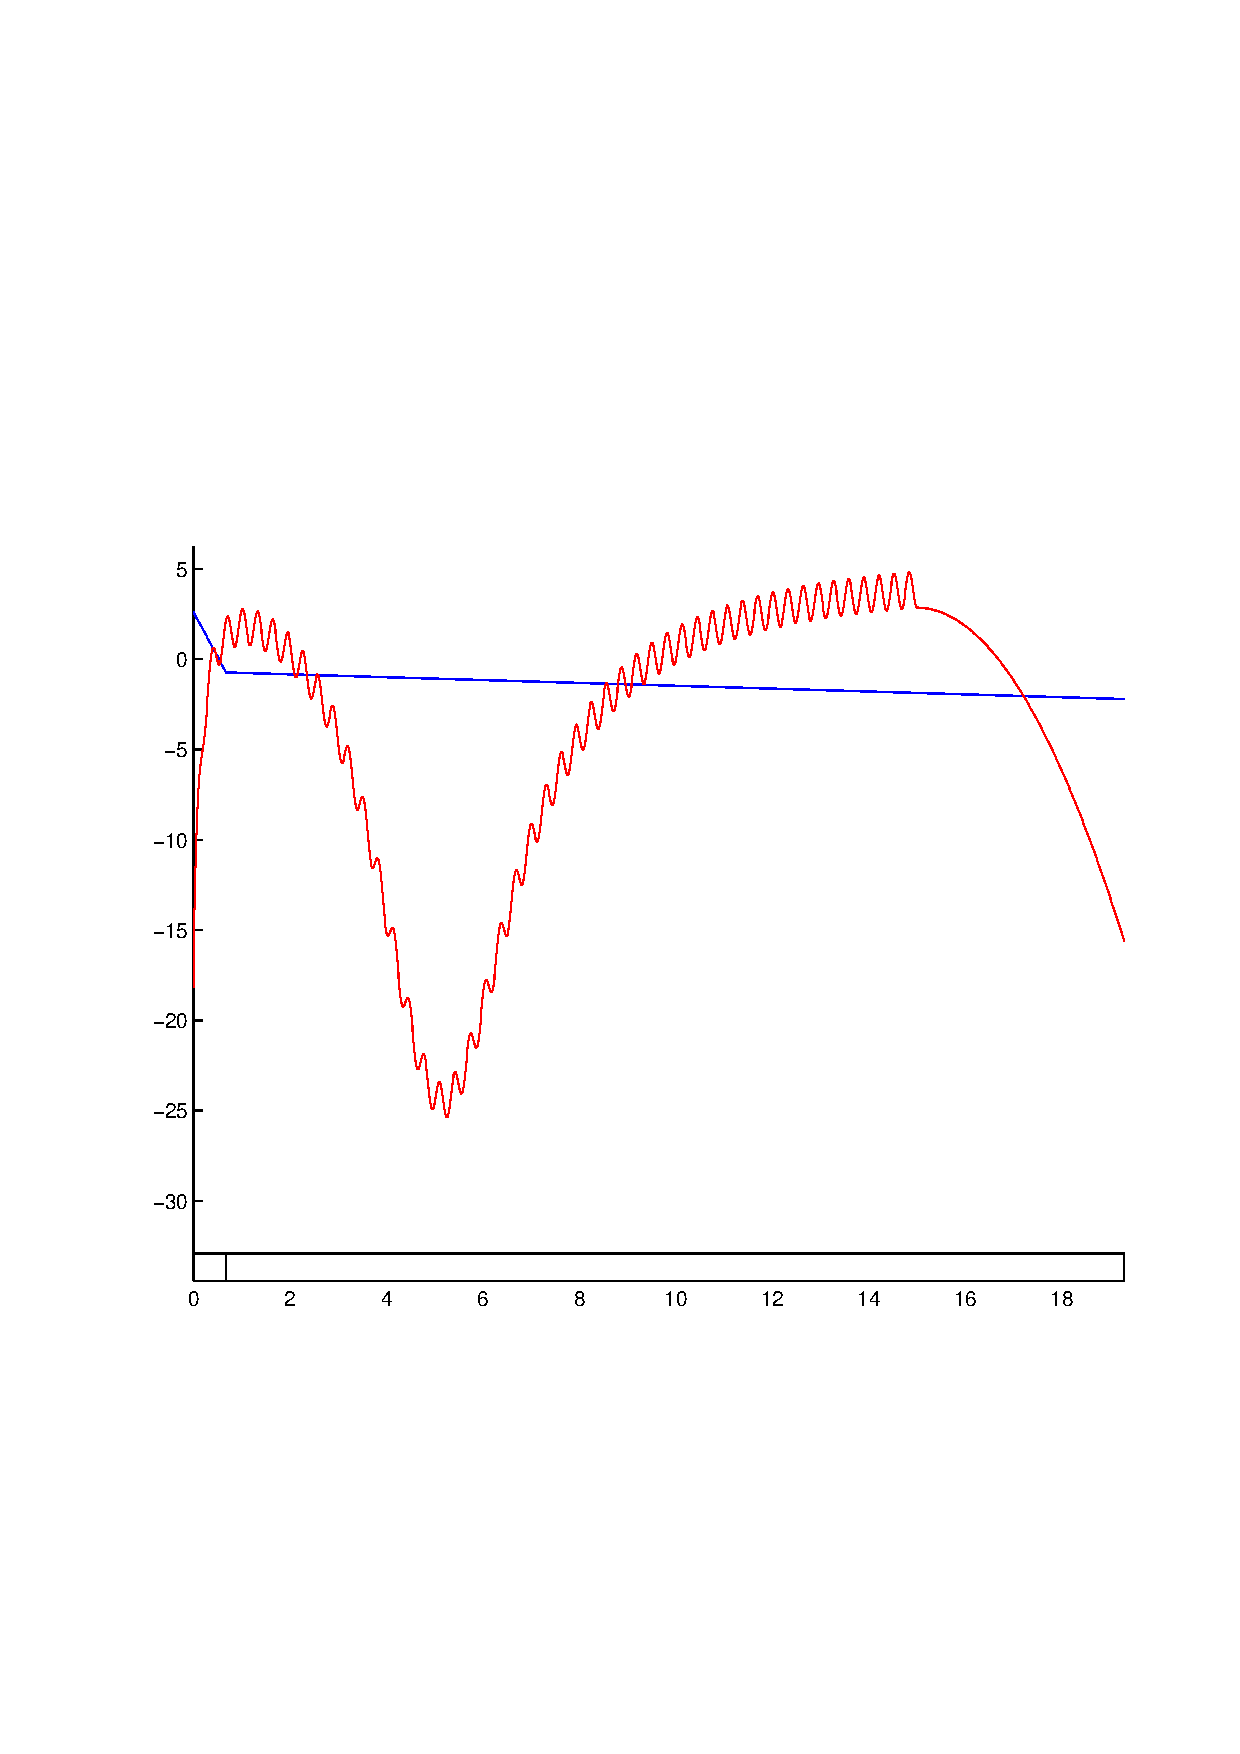
\includegraphics[width=0.3\textwidth]{Figure1}
%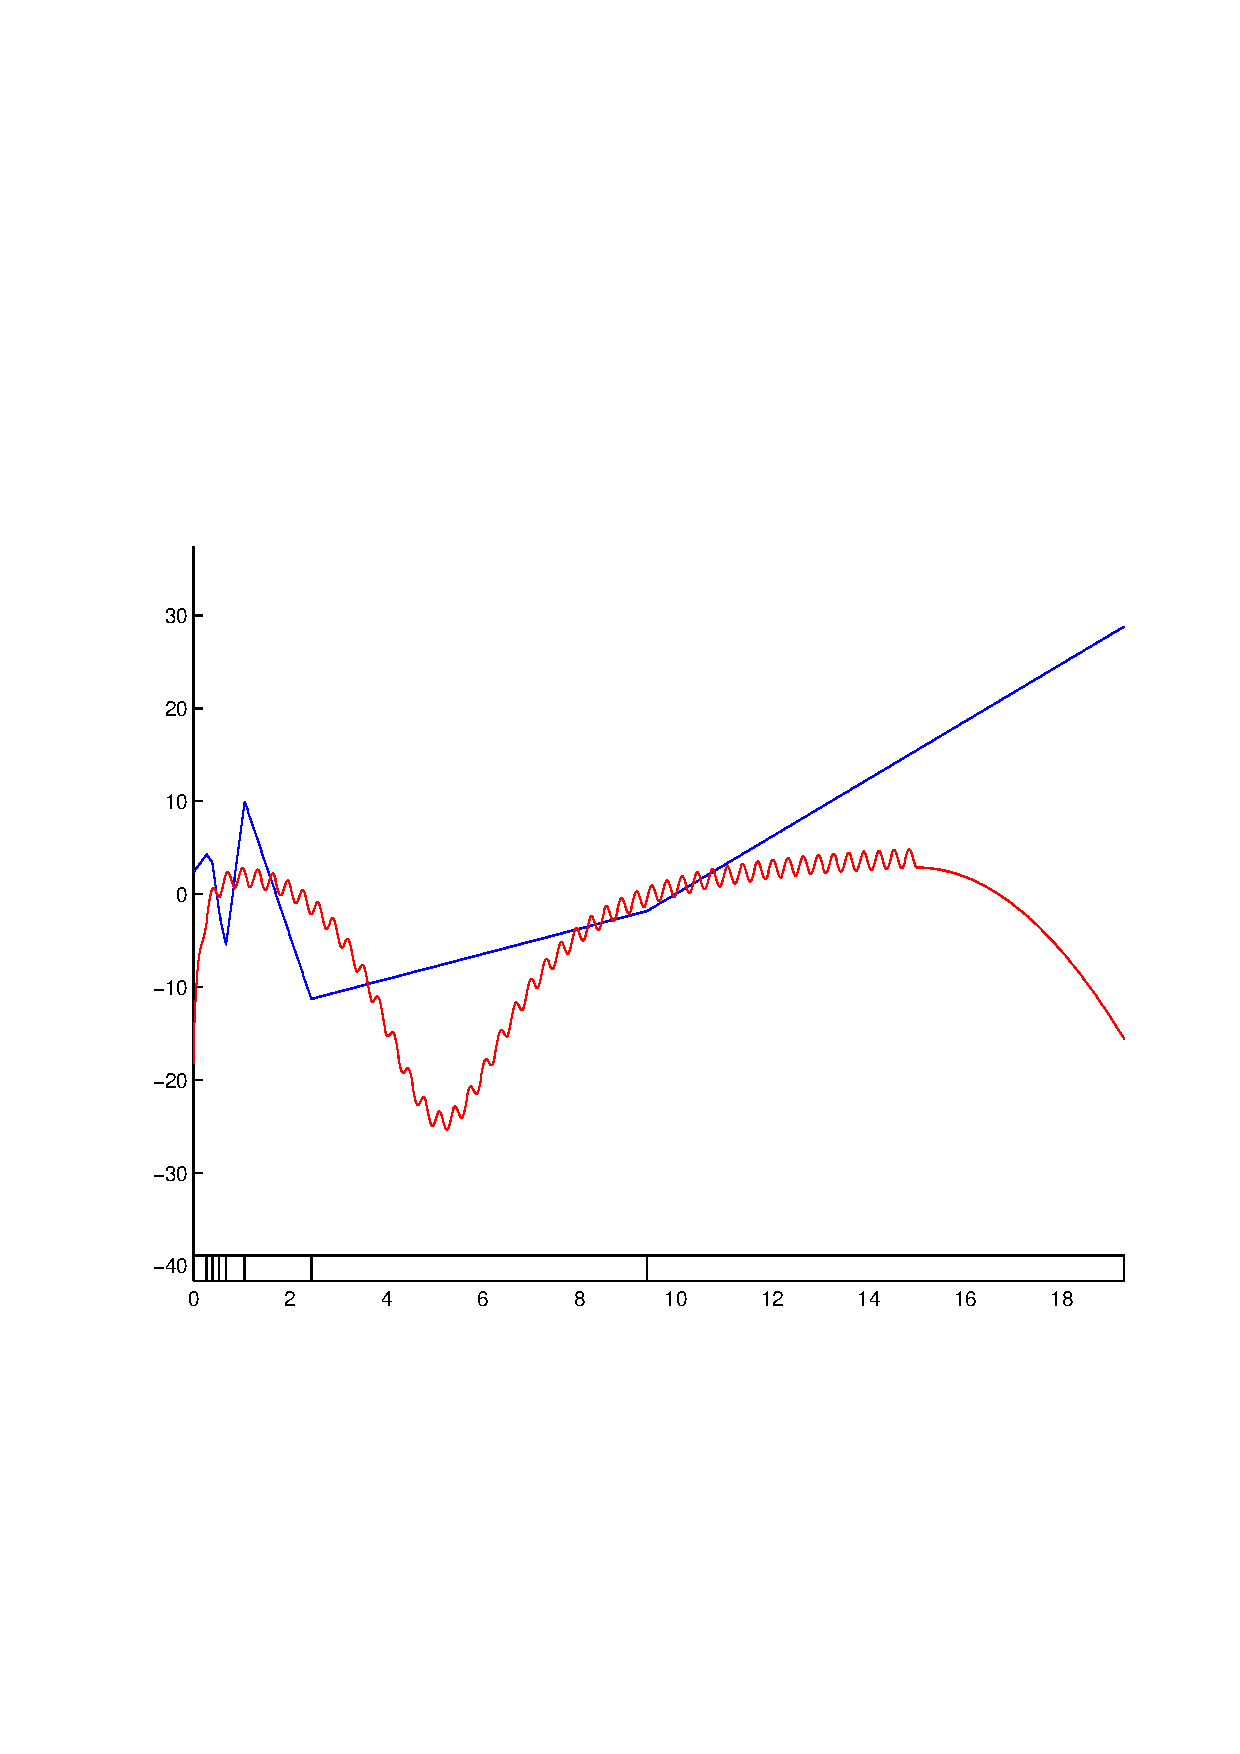
\includegraphics[width=0.3\textwidth]{Figure3}
%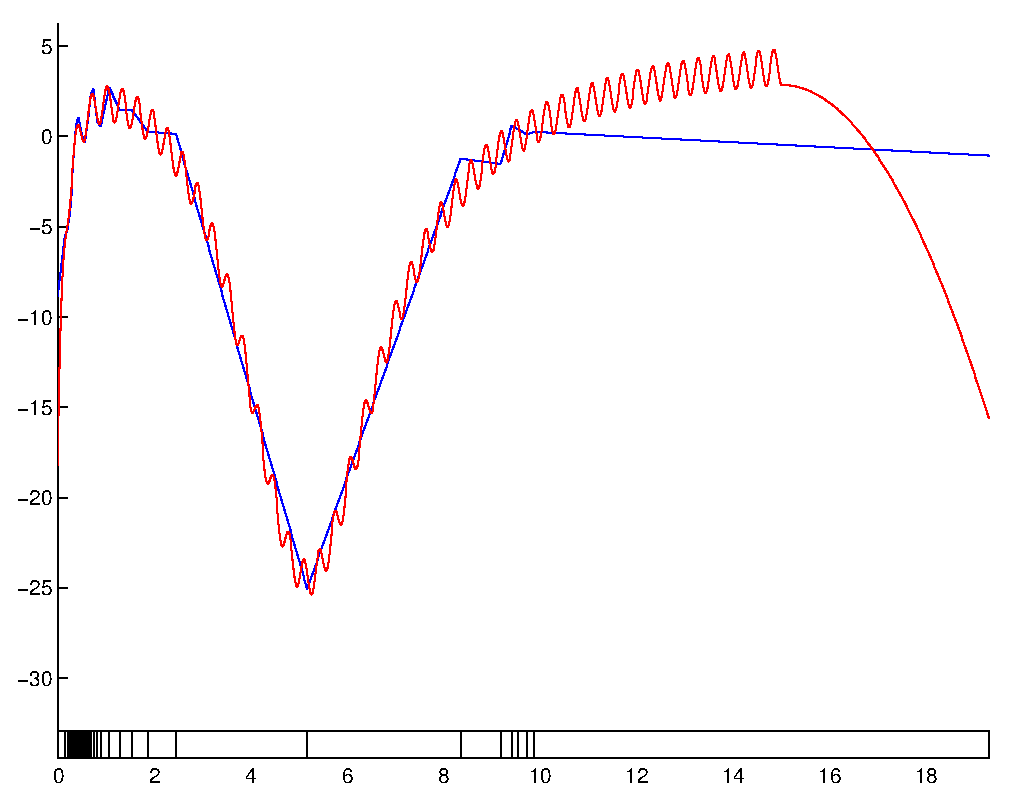
\includegraphics[width=0.3\textwidth]{Figure5}
%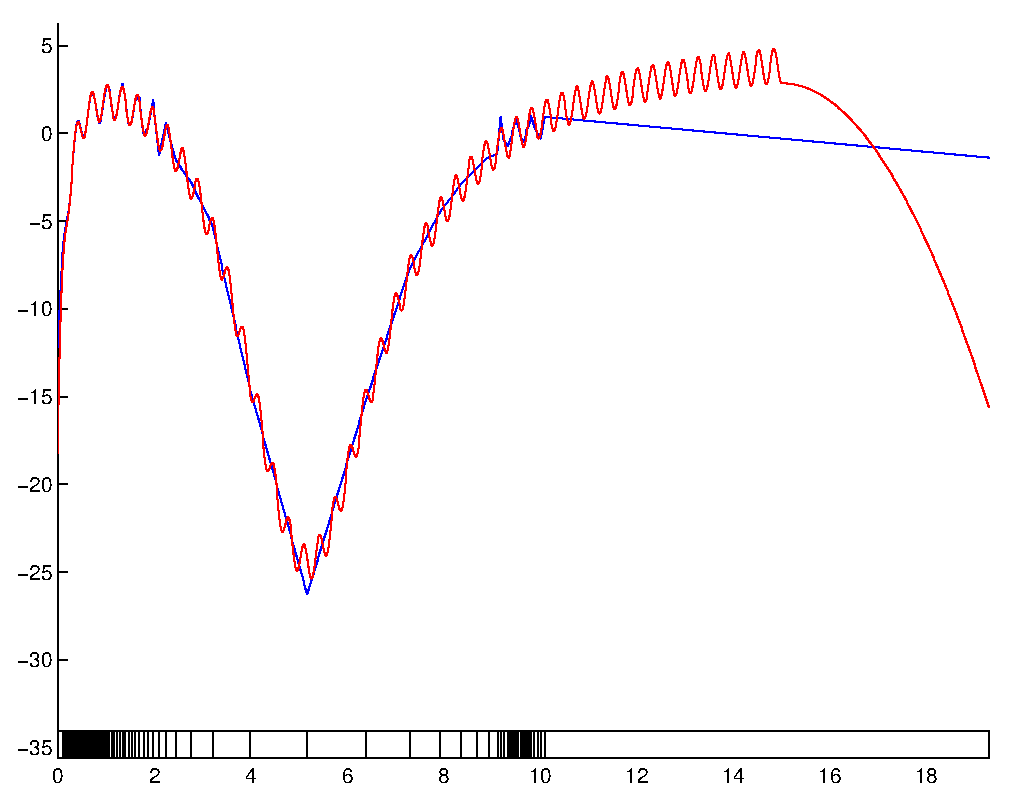
\includegraphics[width=0.3\textwidth]{Figure7}
%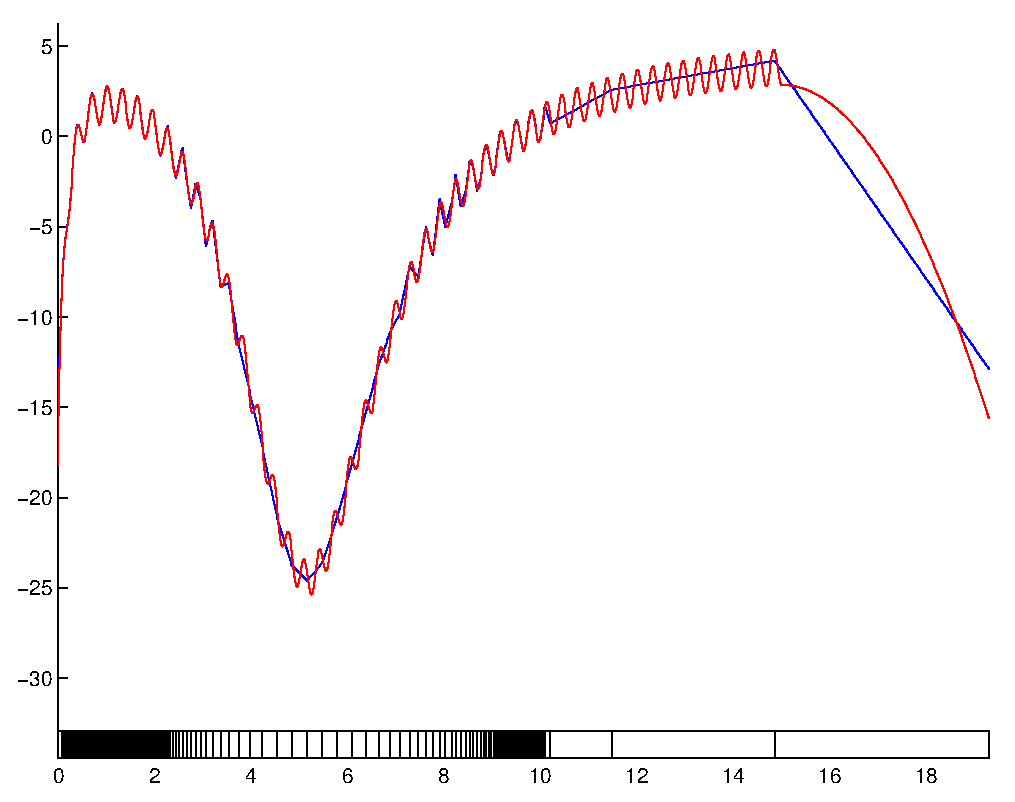
\includegraphics[width=0.3\textwidth]{Figure9}
%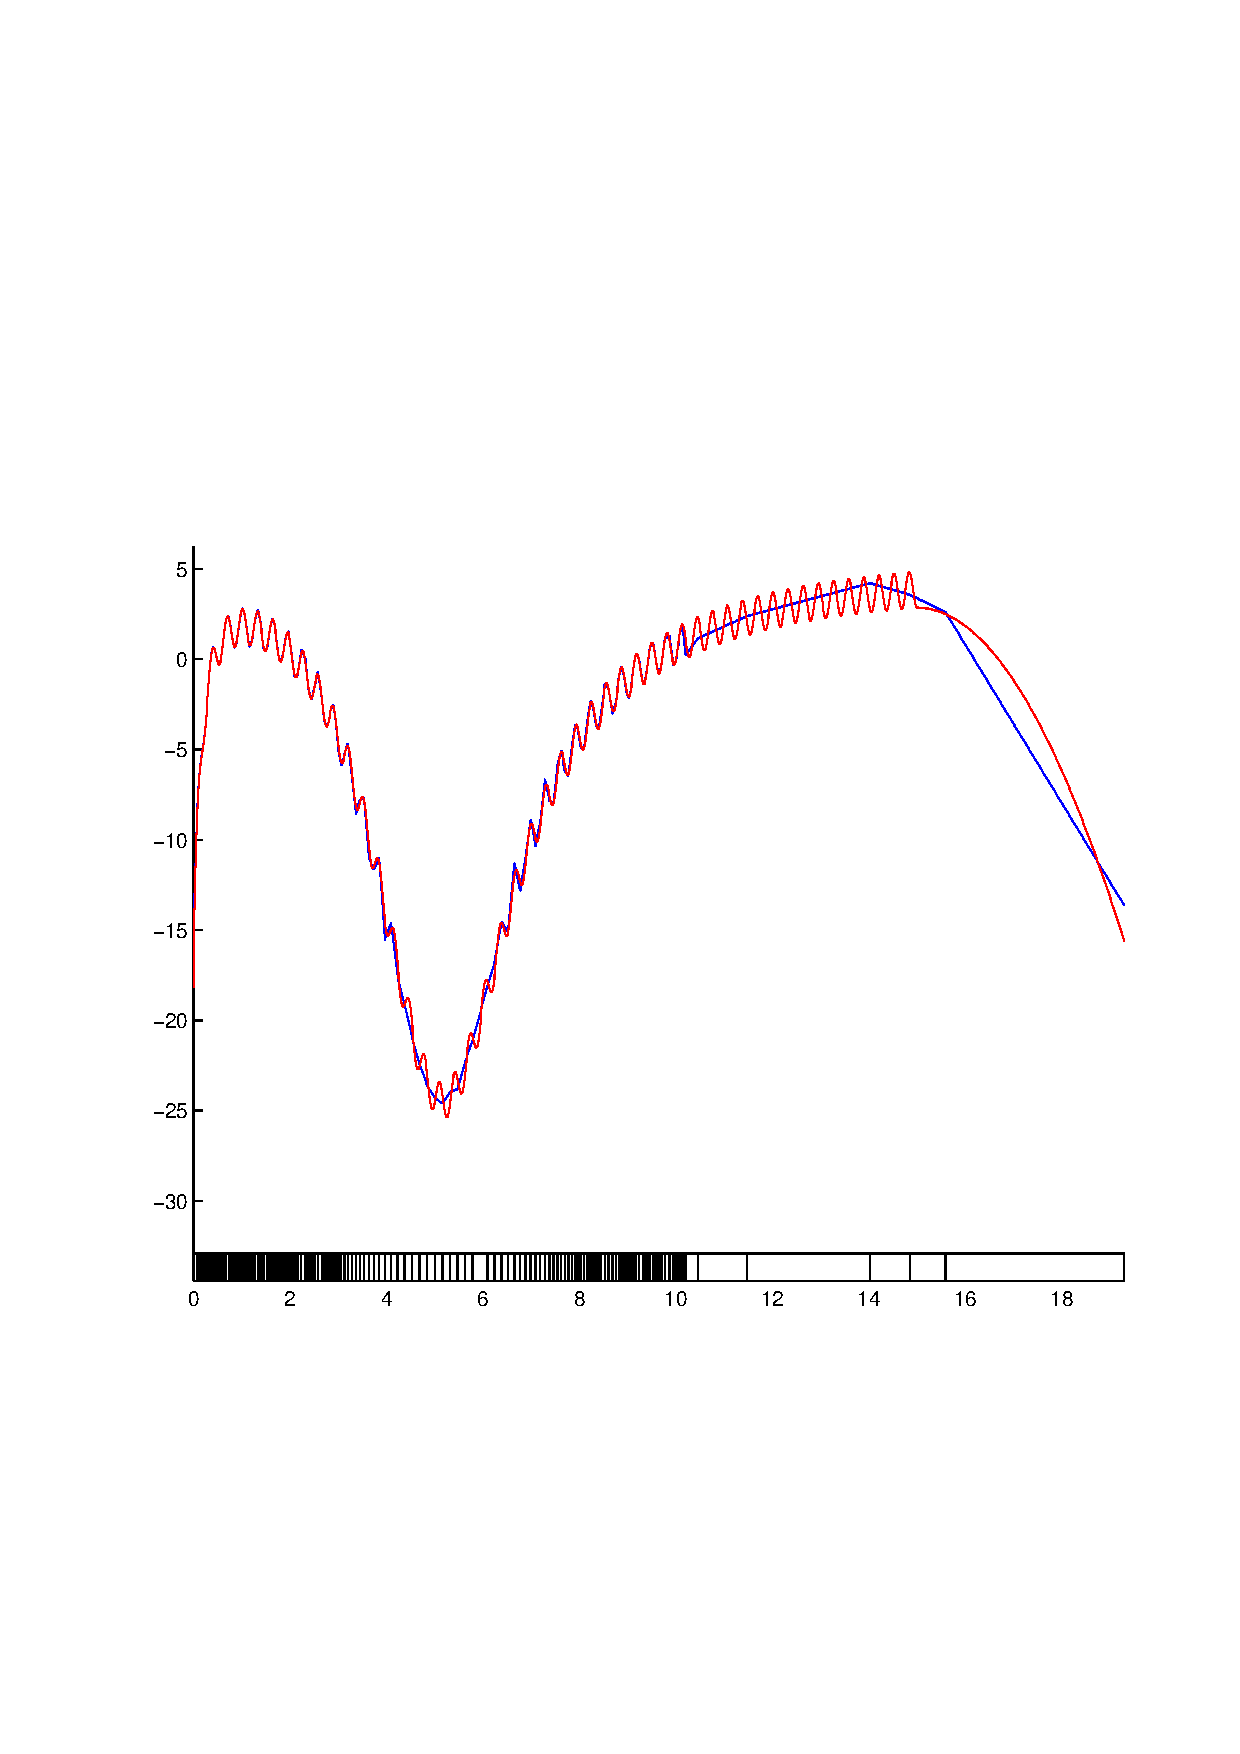
\includegraphics[width=0.3\textwidth]{Figure11} 
%\end{center}
%\caption{First preliminary numerical experiments indicating the successful recovery by an adaptive algorithm based on \eqref{fdproxy} of a potential function $a$ in a first order model of the type \eqref{fdgradientflow}. The potential $a$ to be recovered is displayed in red color and it's the strongly oscillating function. The blue function is the piecewise linear approximant computed at each successive iteration after adaptation of the underlying mesh, scketched on the bottom of the figures.}\label{firstnum}
%\end{figure}
%
%Despite the highly oscillatory nature of the parameter function $a$, the algorithm performs an excellent approximation, providing also a sort of "numerical homogenization" in those locations of the positive real line, where not enough data are provided by the evolution.

In this section we report several numerical experiments to document the validity and feasibility of Theorem \ref{thm}. We will first show how the reconstruction of a kernel gets better as the number of agents $N$ increases, in accordance with the $\Gamma$-convergence result reported in the last section. This feature holds true also for interaction kernel not lying in the function space $X$, as shown in Figure \ref{variableN2}. We will then investigate the relationship between the functional $\mathcal E_N$ and the $L_2(\R_+,\rho)$ error w.r.t. the potential $a$, and the behavior of $\mathcal E_N$ when we let the constraint $M$ vary. Finally, we will see how we can get a very satisfactory reconstruction of the unknown interaction kernel by keeping $N$ fixed and averaging the minimizers of the functional $\mathcal E_N$ obtained from several samples of the initial data distribution $\mu^0$.

\subsection{Numerical framework}\label{numfram}

All experiments will rely on a common numerical set-up, which we clarify in this section. All the initial data $\mu^N_0$ are drawn from a common probability distribution $\mu_0$ which is the uniform distribution on the $d$-dimensional cube $[-L,L]^d$. For every $\mu^N_0$, we simulate the evolution of the system starting from $\mu^N_0$ until time $T$, and we shall denote with $R$ the maximal distance between particles reached during the time frame $[0,T]$. Notice that we have at our disposal only a finite sequence of snapshots of the dynamics: if we denote with $0 = t_0 < t_1 < \ldots < t_m = T$ the time instants at which these snapshots are taken, we can consider the \textit{discrete-time error functional}
\begin{align*}
\overline{\mathcal{E}}_N(\widehat{a}) & = \frac{1}{m} \sum^m_{k = 1} \frac{1}{N} \sum^N_{j = 1} \left| \frac{1}{N} \sum^N_{i = 1} \widehat{a}(|x_j(t_k) - x_i(t_k)|)(x_j(t_k) - x_i(t_k)) - \dot{x}_i(t_k)\right|^2,
\end{align*}
which is the time-discrete counterpart of the continuous-time error functional $\mathcal{E}_N(\widehat{a})$. As already mentioned in the introduction, velocities $\dot{x}_i(t_k)$ appearing in $\overline{\mathcal{E}}_N(\widehat{a})$ are computed as finite differences, i.e.,
\begin{align*}
\dot{x}_i(t_k) = \frac{x_i(t_k) - x_i(t_{k-1})}{t_k - t_{k-1}}, \text{ for every } k \geq 1.
\end{align*}

About the reconstruction procedure, we fix the constraint $M$ and consider the sequence of invading subspaces $V_N$ generated by a linear B-spline basis with $D(N) $ elements supported on $[0,R]$, i.e., for every element $\widehat{a} \in V_N$ it holds
\begin{align*}
	\widehat{a}(r) = \sum^{D(N)}_{\lambda = 1} a_{\lambda} \varphi_{\lambda}(r), \quad \text{for every } r \in [0,R].
\end{align*}
Since $V_N$ has to be invading, $D(N)$ is a strictly increasing function of $N$. To avoid the inconvenience of having a reconstructed kernel with value at $0$ and at $R$ equal to $0$, we consider the knots of the B-spline basis to be
\begin{align}\label{eq:knots}
\left[0,0,0,\frac{R}{(D(N)-2)},\ldots,\frac{(D(N) - 3)R}{(D(N)-2)},R,R,R\right],
\end{align}
i.e., the spline reconstruction has in $0$ and $R$ two discontinuity points.

Whenever $\widehat{a} \in V_N$, we can rewrite the functional $\mathcal{E}_N(\widehat{a})$ as
\begin{align*}
\overline{\mathcal{E}}_N(\widehat{a}) & = \frac{1}{m} \sum^m_{k = 1} \frac{1}{N} \sum^N_{j = 1} \left| \frac{1}{N} \sum^N_{i = 1} \sum^{D(N)}_{\lambda = 1} a_{\lambda} \varphi_{\lambda}(|x_j(t_k) - x_i(t_k)|)(x_j(t_k) - x_i(t_k)) - \dot{x}_i(t_k)\right|^2 \\
& = \frac{1}{m} \sum^m_{k = 1} \frac{1}{N} \sum^N_{j = 1} \left| \sum^{D(N)}_{\lambda = 1} a_{\lambda} \frac{1}{N} \sum^N_{i = 1} \varphi_{\lambda}(|x_j(t_k) - x_i(t_k)|)(x_j(t_k) - x_i(t_k)) - \dot{x}_i(t_k)\right|^2 \\
& = \frac{1}{mN} \left\| C \vec{a} - v \right\|^2_{2},
\end{align*}
where $\vec{a} = (a_1, \ldots, a_{D(N)})$, $v = (\dot{x}_1(t_1), \ldots, \dot{x}_N(t_1), \ldots,\dot{x}_1(t_m), \ldots, \dot{x}_N(t_m))$ and $C \in \R^{d\times Nm \times D(N)}$ satisfies for every $j = 1, \ldots,N$, $k = 1, \ldots,m$, $\lambda = 1, \ldots,D(N)$
\begin{align*}
C(jk,\lambda) = \frac{1}{N} \sum^N_{i = 1} \varphi_{\lambda}(|x_j(t_k) - x_i(t_k)|)(x_j(t_k) - x_i(t_k)) \in \R^d.
\end{align*}

We shall numerically implement the constrained minimization with the software CVX, which allows constraints and objectives to be specified using standard MATLAB expression syntax. In order to use it, we need to rewrite the constraint of our minimization problem, which reads
\begin{align*}
	\|a\|_{L_{\infty}([0,R])} + \|a'\|_{L_{\infty}([0,R])} \leq M,
\end{align*}
using only the minimization variable of the problem, which is the vector of coefficients of the B-spline basis $\vec{a}$. Notice that the property of being a linear B-spline basis implies that, for every $\lambda = 1, \ldots, D(N)-1$, the property $\supp(\varphi_{\lambda}) \cap \supp(\varphi_{\lambda + j}) \not= \emptyset$ holds if and only if $j = 1$. Hence, for every $a \in V_N$ we have
\begin{align*}
\|a\|_{L_{\infty}([0,R])} &= \max_{r \in [0,R]} \left|\sum^{D(N)}_{\lambda = 1} a_{\lambda} \varphi_{\lambda}(r)\right| \\
& \leq \max_{r \in [0,R]} \sum^{D(N)}_{\lambda = 1} \left|a_{\lambda} \varphi_{\lambda}(r)\right| \\
& \leq \max_{\lambda = 1, \ldots, D(N)-1} \left(|a_{\lambda}| + |a_{\lambda+1}|\right) \\
& \leq 2 \|\vec{a}\|_{\infty},
\end{align*}
\begin{align*}
\|a'\|_{L_{\infty}([0,R])} &= \max_{r \in [0,R]} \left|\sum^{D(N)}_{\lambda = 1} a_{\lambda} \varphi'_{\lambda}(r)\right| \\
& \leq \max_{\lambda = 1, \ldots, D(N)-1} |a_{\lambda+1} - a_{\lambda}| \\
& = \|D\vec{a}\|_{\infty},
\end{align*}
where, in the last line, $D$ is the matrix
\begin{align*}
D = \begin{bmatrix}
    1       & -1 & 0 & \dots & 0 & 0 \\
    0     & 1 & -1 & \dots & 0 & 0 \\
   \vdots & \vdots & \ddots & \ddots & \vdots & \vdots \\ \\
    0       & 0 & 0 & \dots & 1 & -1 \\
    0       & 0 & 0 & \dots & 0 & 0
\end{bmatrix}.
\end{align*}
Therefore, we numerically implement the constrained minimization problem
\begin{align*}
\min_{\widehat{a} \in V_N} \mathcal{E}_N(\widehat{a}) \quad \text{ subject to } \quad \|\widehat{a}\|_{L_{\infty}([0,R])} + \|\widehat{a}'\|_{L_{\infty}([0,R])} \leq M,
\end{align*}
in the following way
\begin{align}\label{problem2}
\min_{\vec{a} \in \R^{D(N)}} \frac{1}{mN} \left\| C \vec{a} - v \right\|^2_{2} \quad \text{ subject to } \quad 2\|\vec{a}\|_{\infty} + \|D\vec{a}\|_{\infty} \leq M.
\end{align}
The byproduct of the time discretization and the reformulation of the constraint is that minimizers of problem \eqref{problem2} may not be minimizers of the original one. This is the price to pay for the numerical implementation of the theoretical result. However, we will see how in practice the modifications we made are so mild that we always obtain a very satisfactory reconstruction of the unknown potential, and moreover we still observe the approximation properties proved in the previous sections.

\subsection{Varying $N$}

In Figure \ref{variableN} we show the reconstruction of a truncated Lennard-Jones type interaction kernel obtained with different values of $N$. The following table reports the values of the different problem's parameters.

\begin{table}[h]
\begin{center}
\begin{tabular}{ |c|c|c|c|c|c| }
\hline
  $d$ & $L$ & $T$ & $M$ & $N$ & $D(N)$ \\
\hline
\hline
  $2$ & $3$ & $0.5$ & $100$ & $[10,20,40,80]$ & $2N$ \\
\hline
\end{tabular}
\end{center}
\vspace{-0.5cm}
\caption{Parameter values for Figure \ref{variableN} and Figure \ref{variableN2}} \label{tab:fig1} 
\end{table}

It is clearly visible how the the piecewise linear approximant (displayed in blue) gets closer and closer to the potential to be recovered (in red), as predicted by the theoretical results of the previous sections. What is however surprising is that the same behavior is witnessed in Figure \ref{variableN2}, where the algorithm is applied to an interaction kernel $a$ not belonging to the function space $X$ (due to its singularity at the origin) with the same specifications reported in Table \ref{tab:fig1}. The algorithm performs an excellent approximation despite the highly oscillatory nature of the function $a$.

\begin{figure}[h!]
\begin{center}
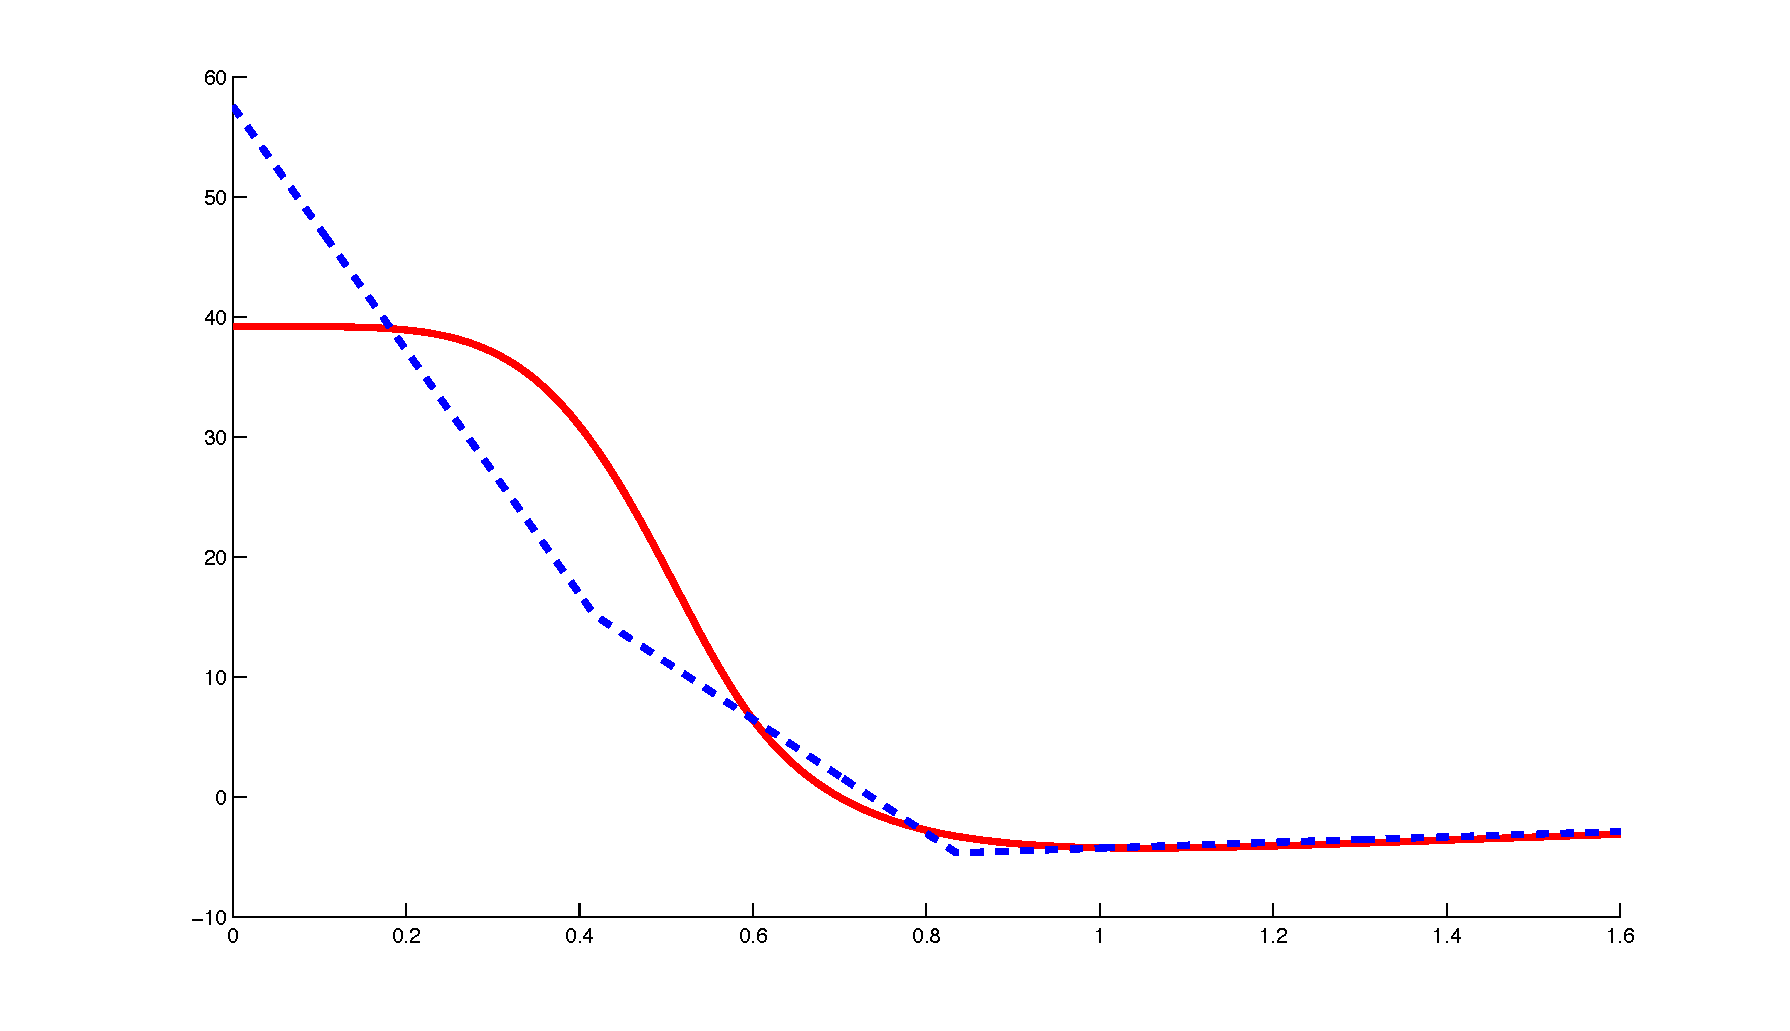
\includegraphics[width=0.45\textwidth]{figfun810agents}
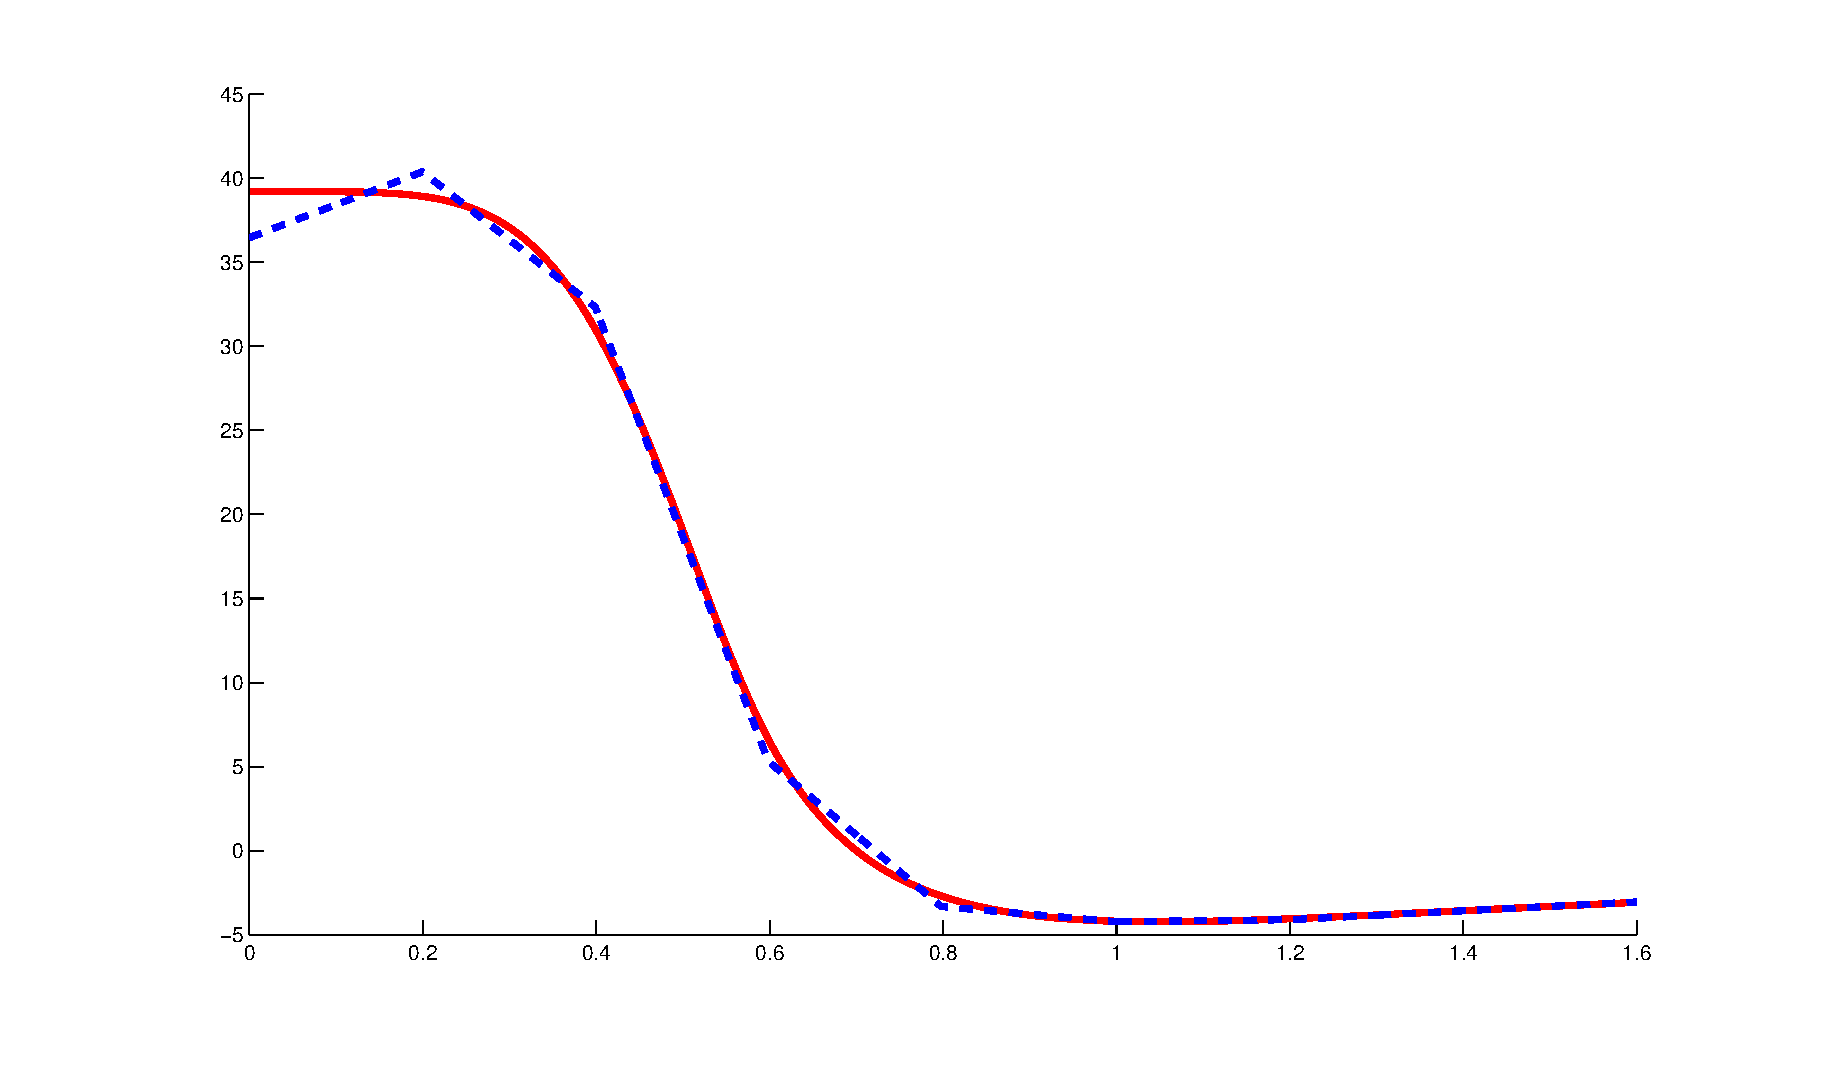
\includegraphics[width=0.45\textwidth]{figfun820agents}\\
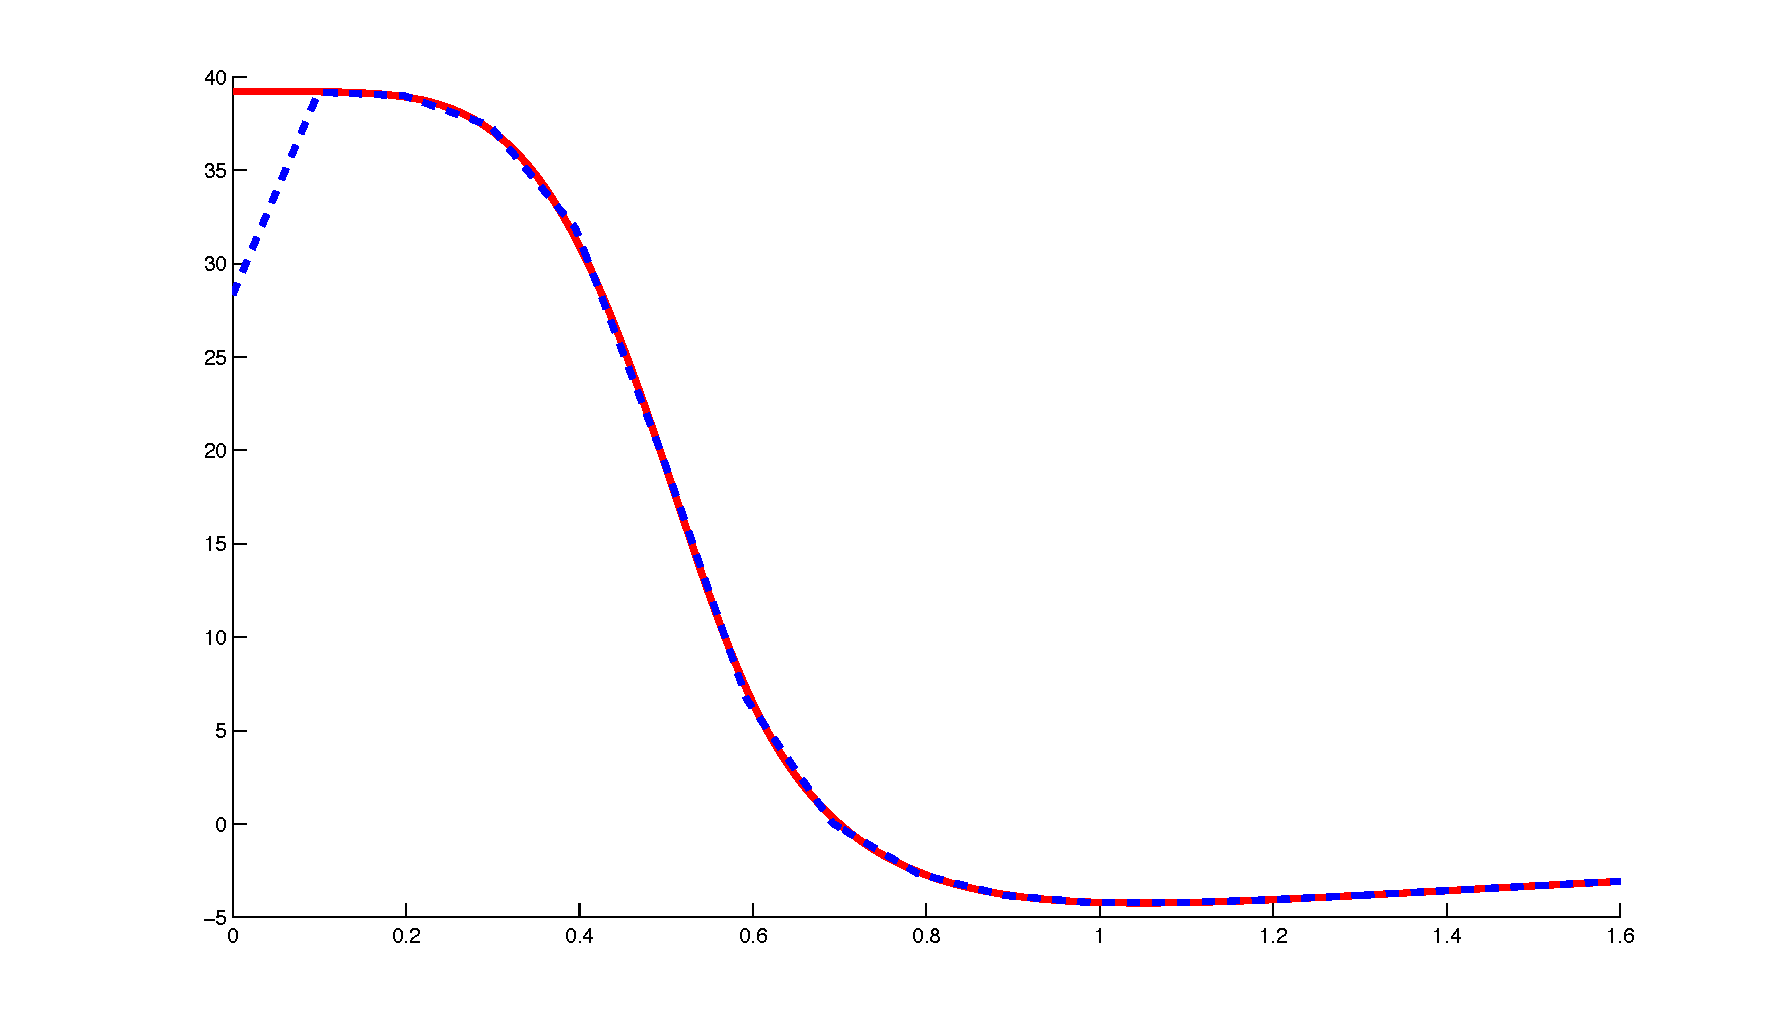
\includegraphics[width=0.45\textwidth]{figfun840agents}
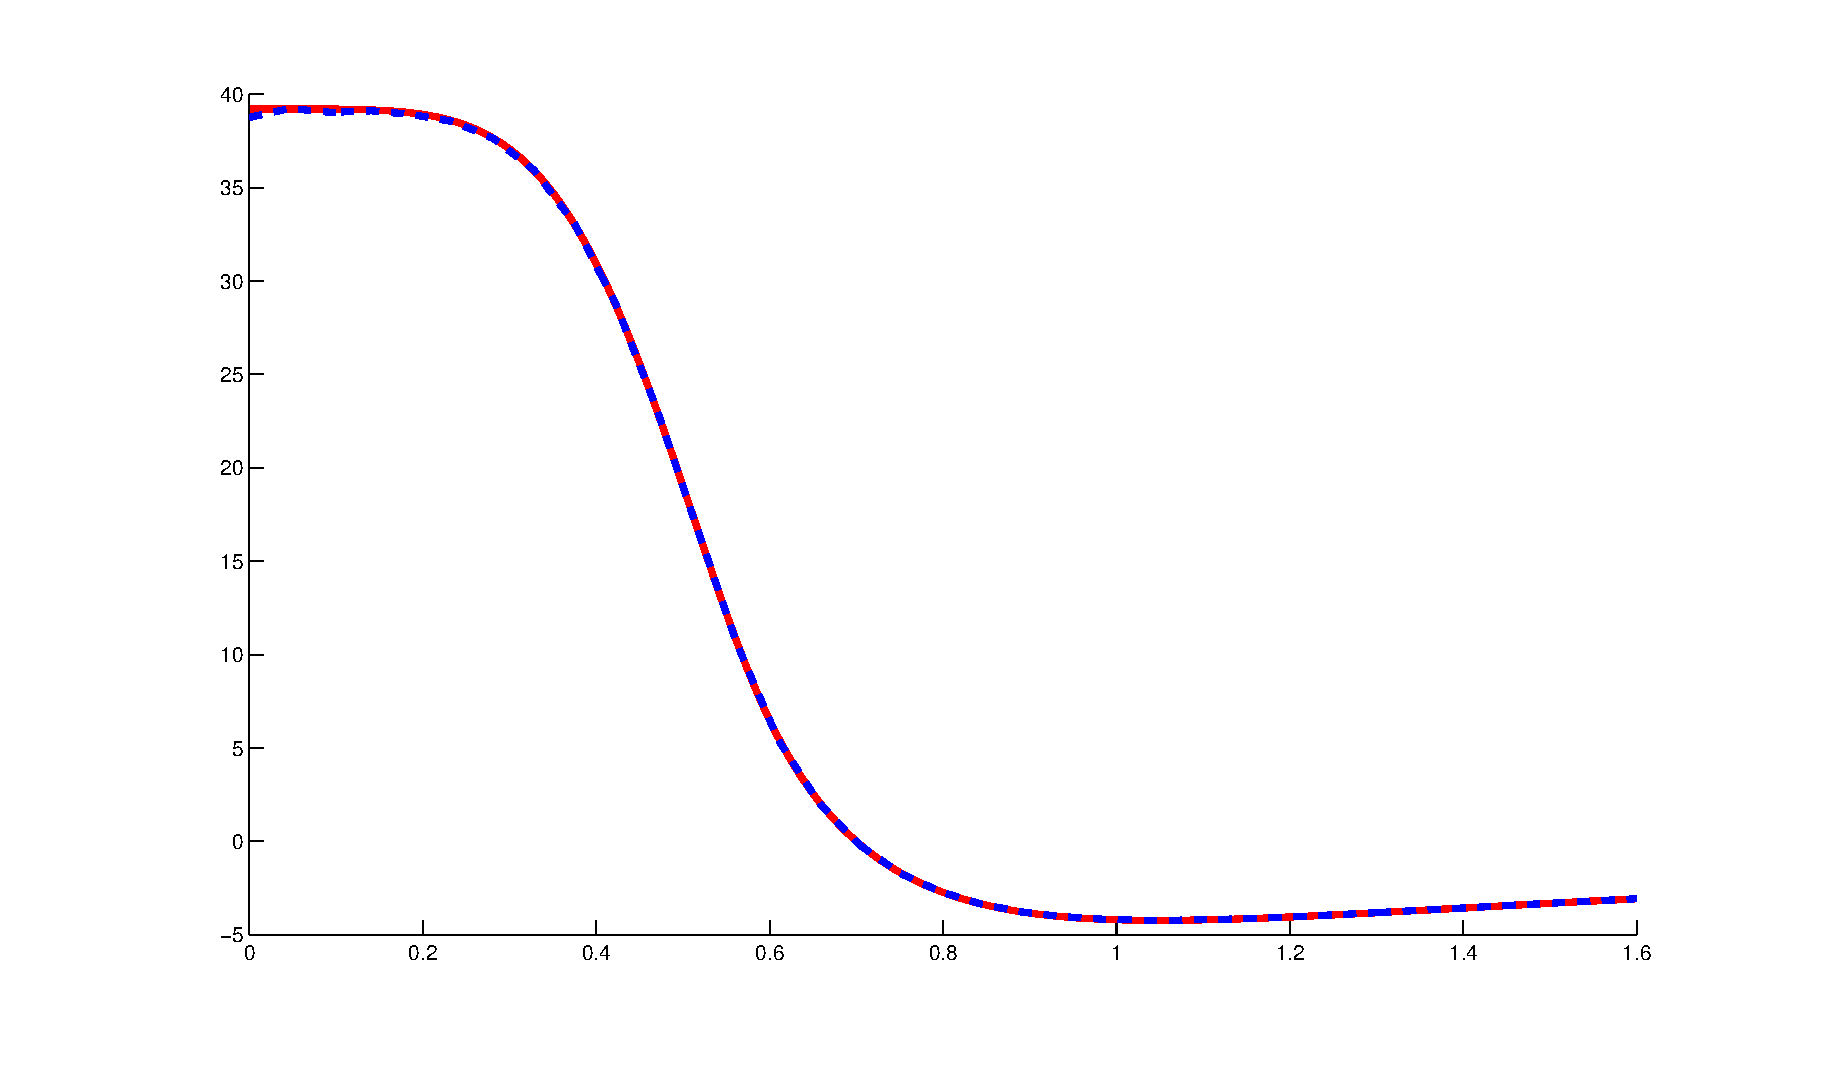
\includegraphics[width=0.45\textwidth]{figfun880agents}
\end{center}
\caption{Iterative reconstruction of a potential with different values of $N$. In red: the unknown kernel. In blue: its reconstruction by minimization of $\mathcal{E}_N$. From left-top to right-bottom: reconstruction with $N = 10$, $N = 20$, $N = 40$, $N = 80$ agents.}\label{variableN}
\end{figure}

\begin{figure}[h!]
\begin{center}
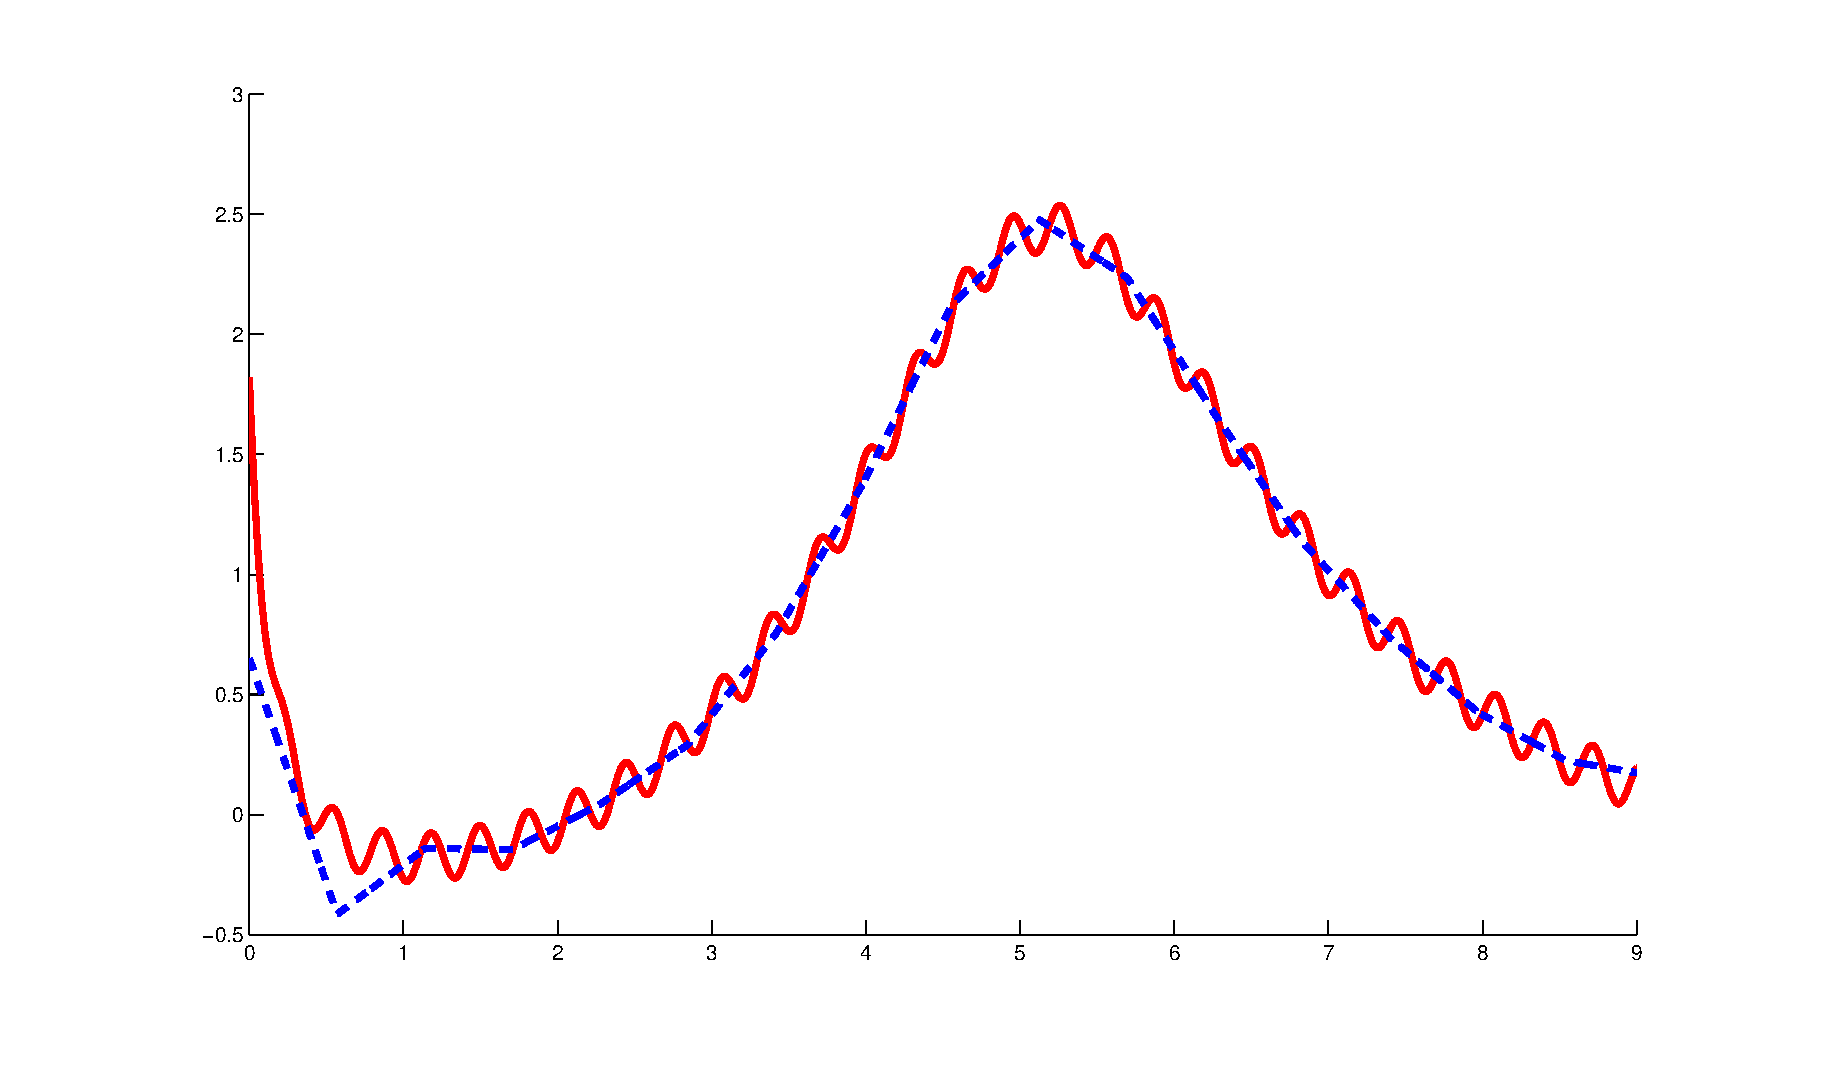
\includegraphics[width=0.45\textwidth]{figfun610agents}
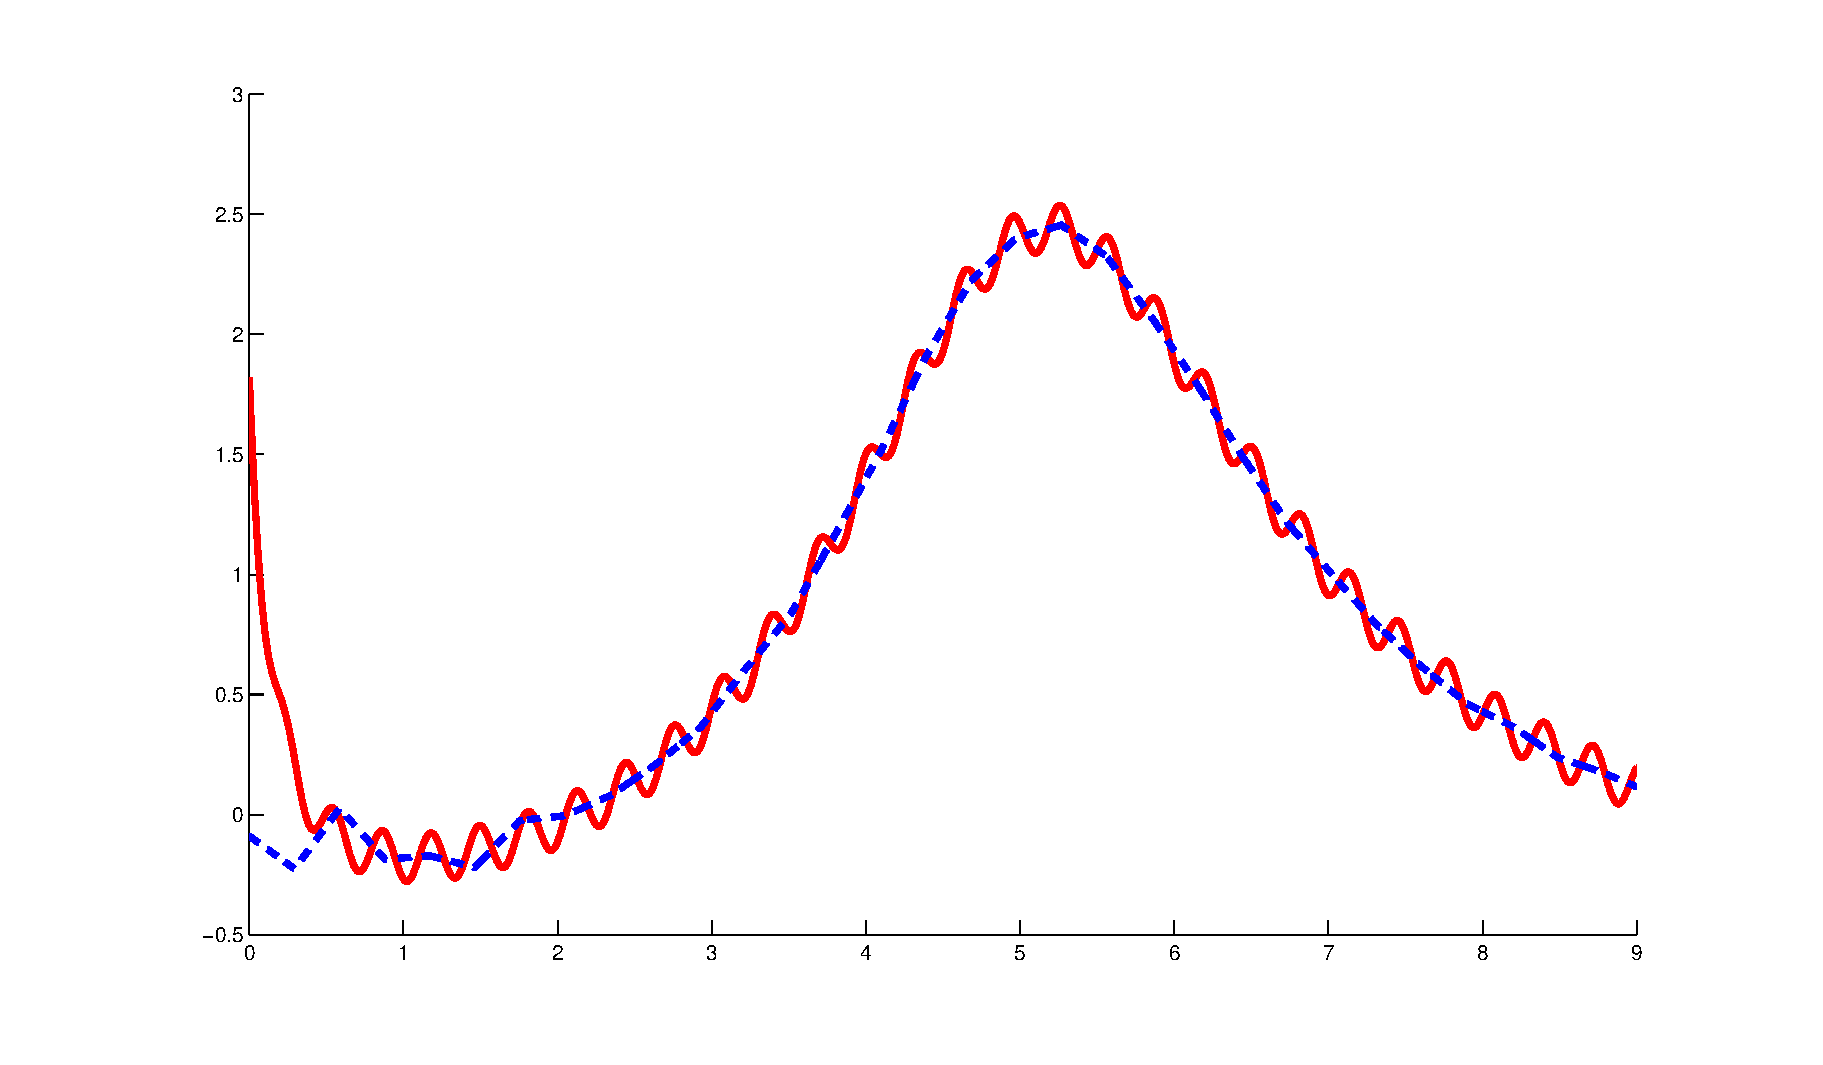
\includegraphics[width=0.45\textwidth]{figfun620agents}\\
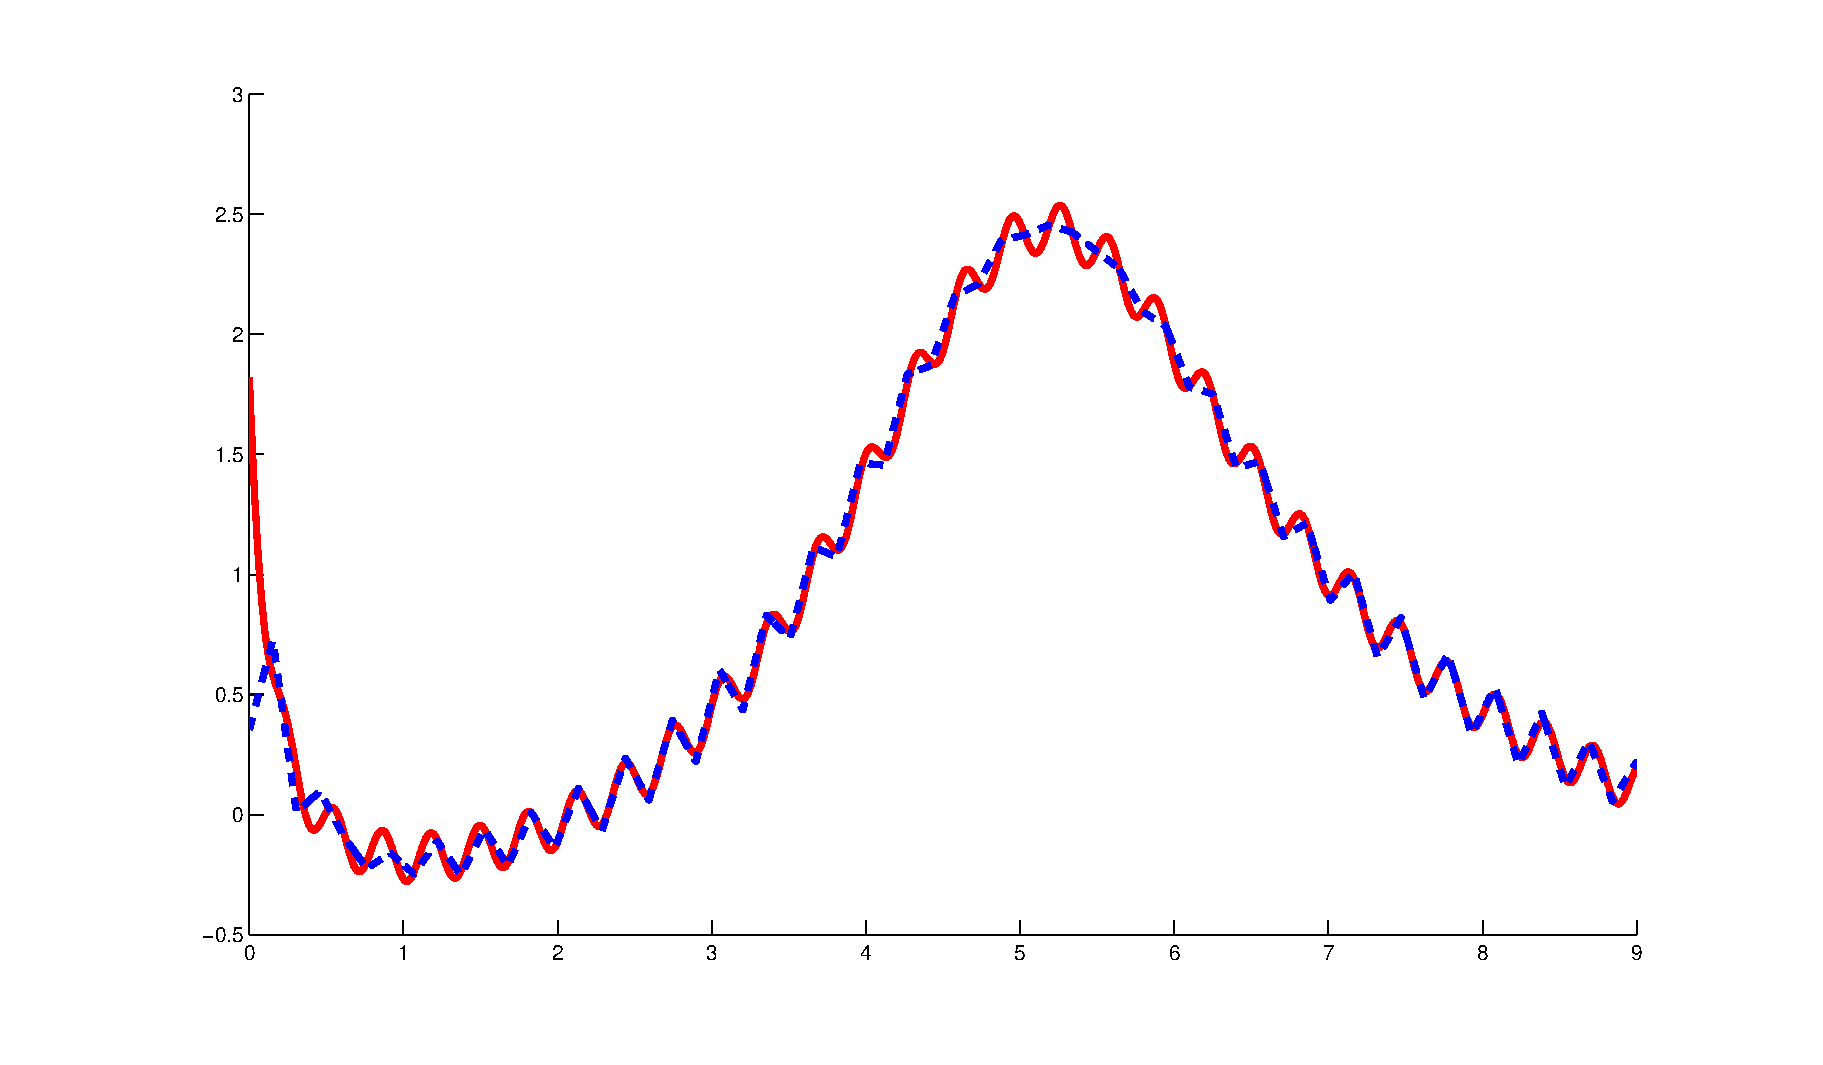
\includegraphics[width=0.45\textwidth]{figfun640agents}
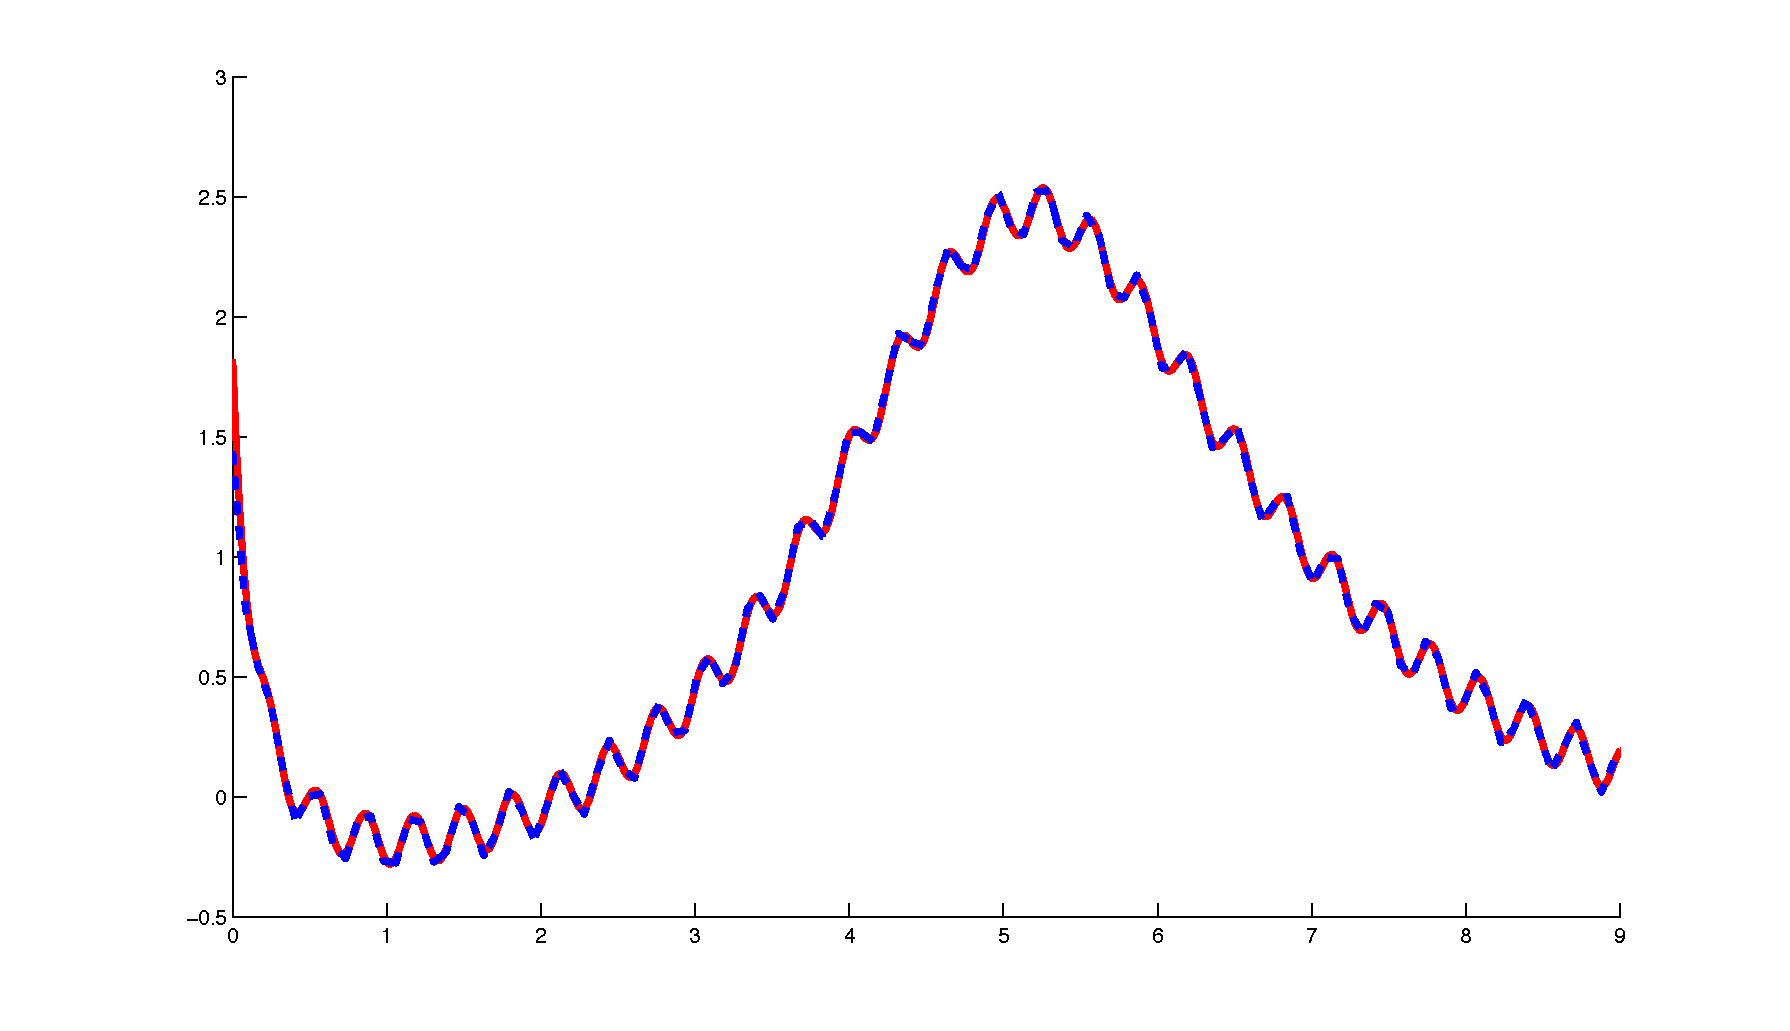
\includegraphics[width=0.45\textwidth]{figfun680agents}
\end{center}
\caption{Iterative reconstruction of a potential with a singularity at the origin and highly oscillatory behavior. In red: the unknown kernel. In blue: its reconstruction by minimization of $\mathcal{E}_N$. From left-top to right-bottom: reconstruction with $N = 10$, $N = 20$, $N = 40$, $N = 80$ agents.}\label{variableN2}
\end{figure}

\subsection{The coercivity constant}

We now turn our attention to the coercivity constant $c_T$ appearing in \eqref{coercivity} and thoroughly discussed in Section \ref{sec:coerc}. In Figure \ref{errorN} we see a comparison between the evolution of the value of the error functional $\overline{\mathcal{E}}_N(\widehat{a}_N)$ and of the $L_2(\R_+,\rho)$-error $\|a-\widehat{a}_N\|^2_{L_2(\R_+,\rho)}$ for different values of $N$. 

\begin{figure}[h]
\hspace{-1.2cm}
\begin{minipage}{0.58\textwidth}
\begin{center}
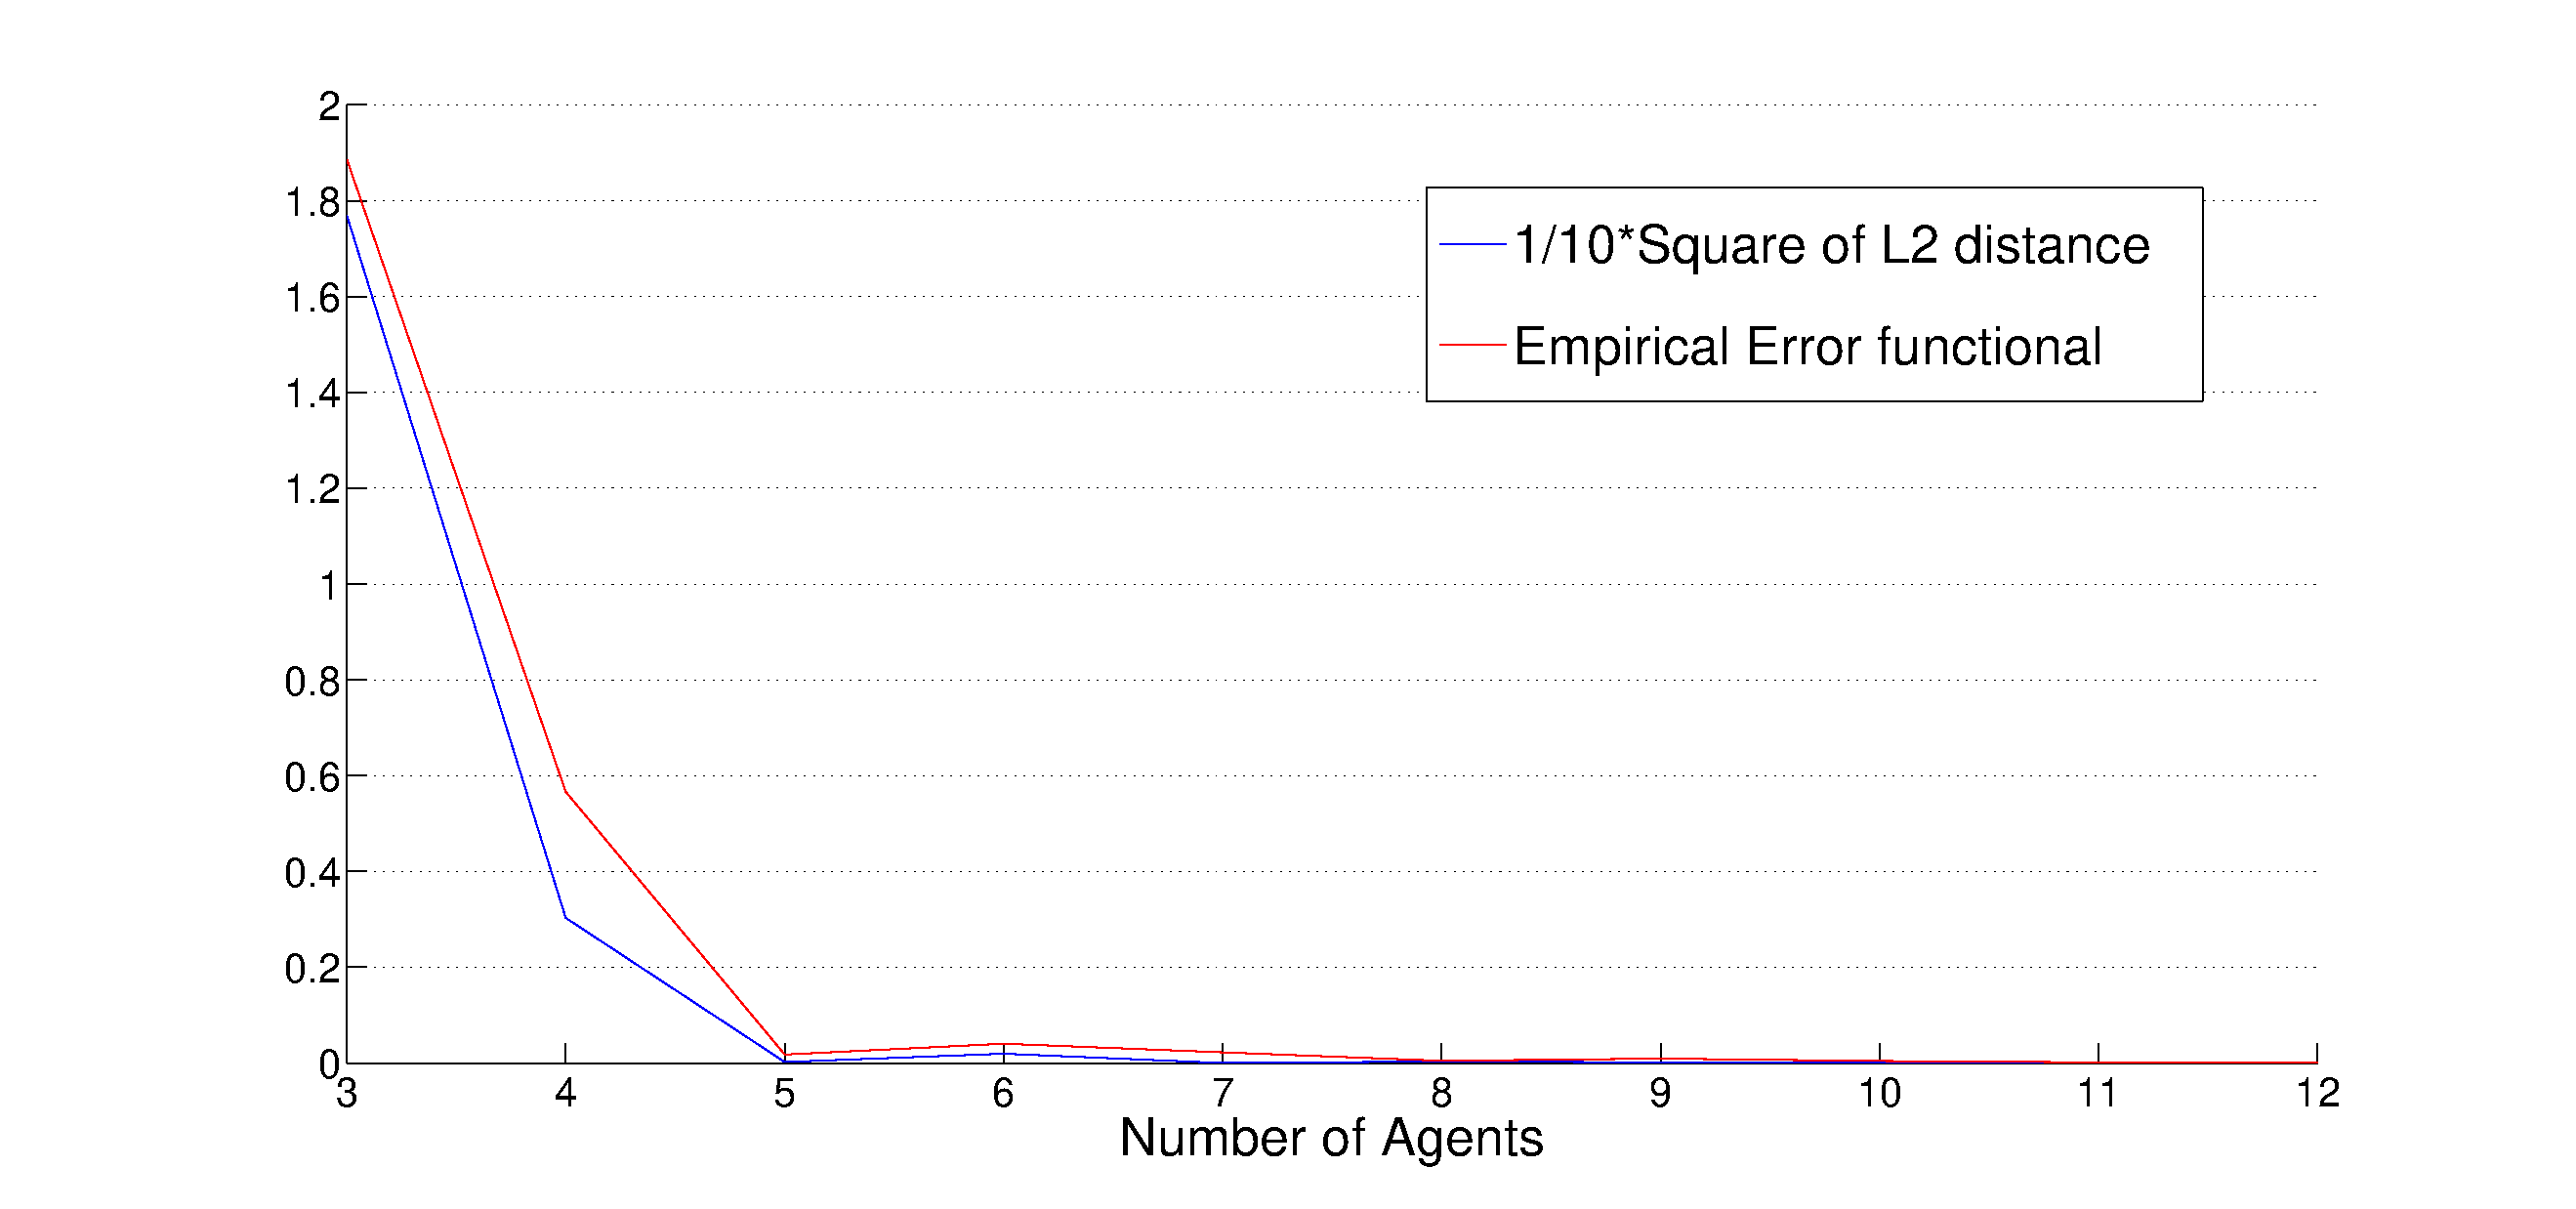
\includegraphics[width=1\textwidth]{figErrorN.eps}
\end{center}
\caption{Plot of $\overline{\mathcal{E}}_N(\widehat{a}_N)$ and $\frac{1}{10}\|a-\widehat{a}_N\|^2_{L_2(\R_+,\rho)}$ for different values of $N$. In this experiment, we can estimate the constant $c_T$ with the value $\frac{1}{10}$.}\label{errorN}
\end{minipage}
\hspace{0.4cm}
\begin{minipage}{0.55\textwidth}
\begin{center}
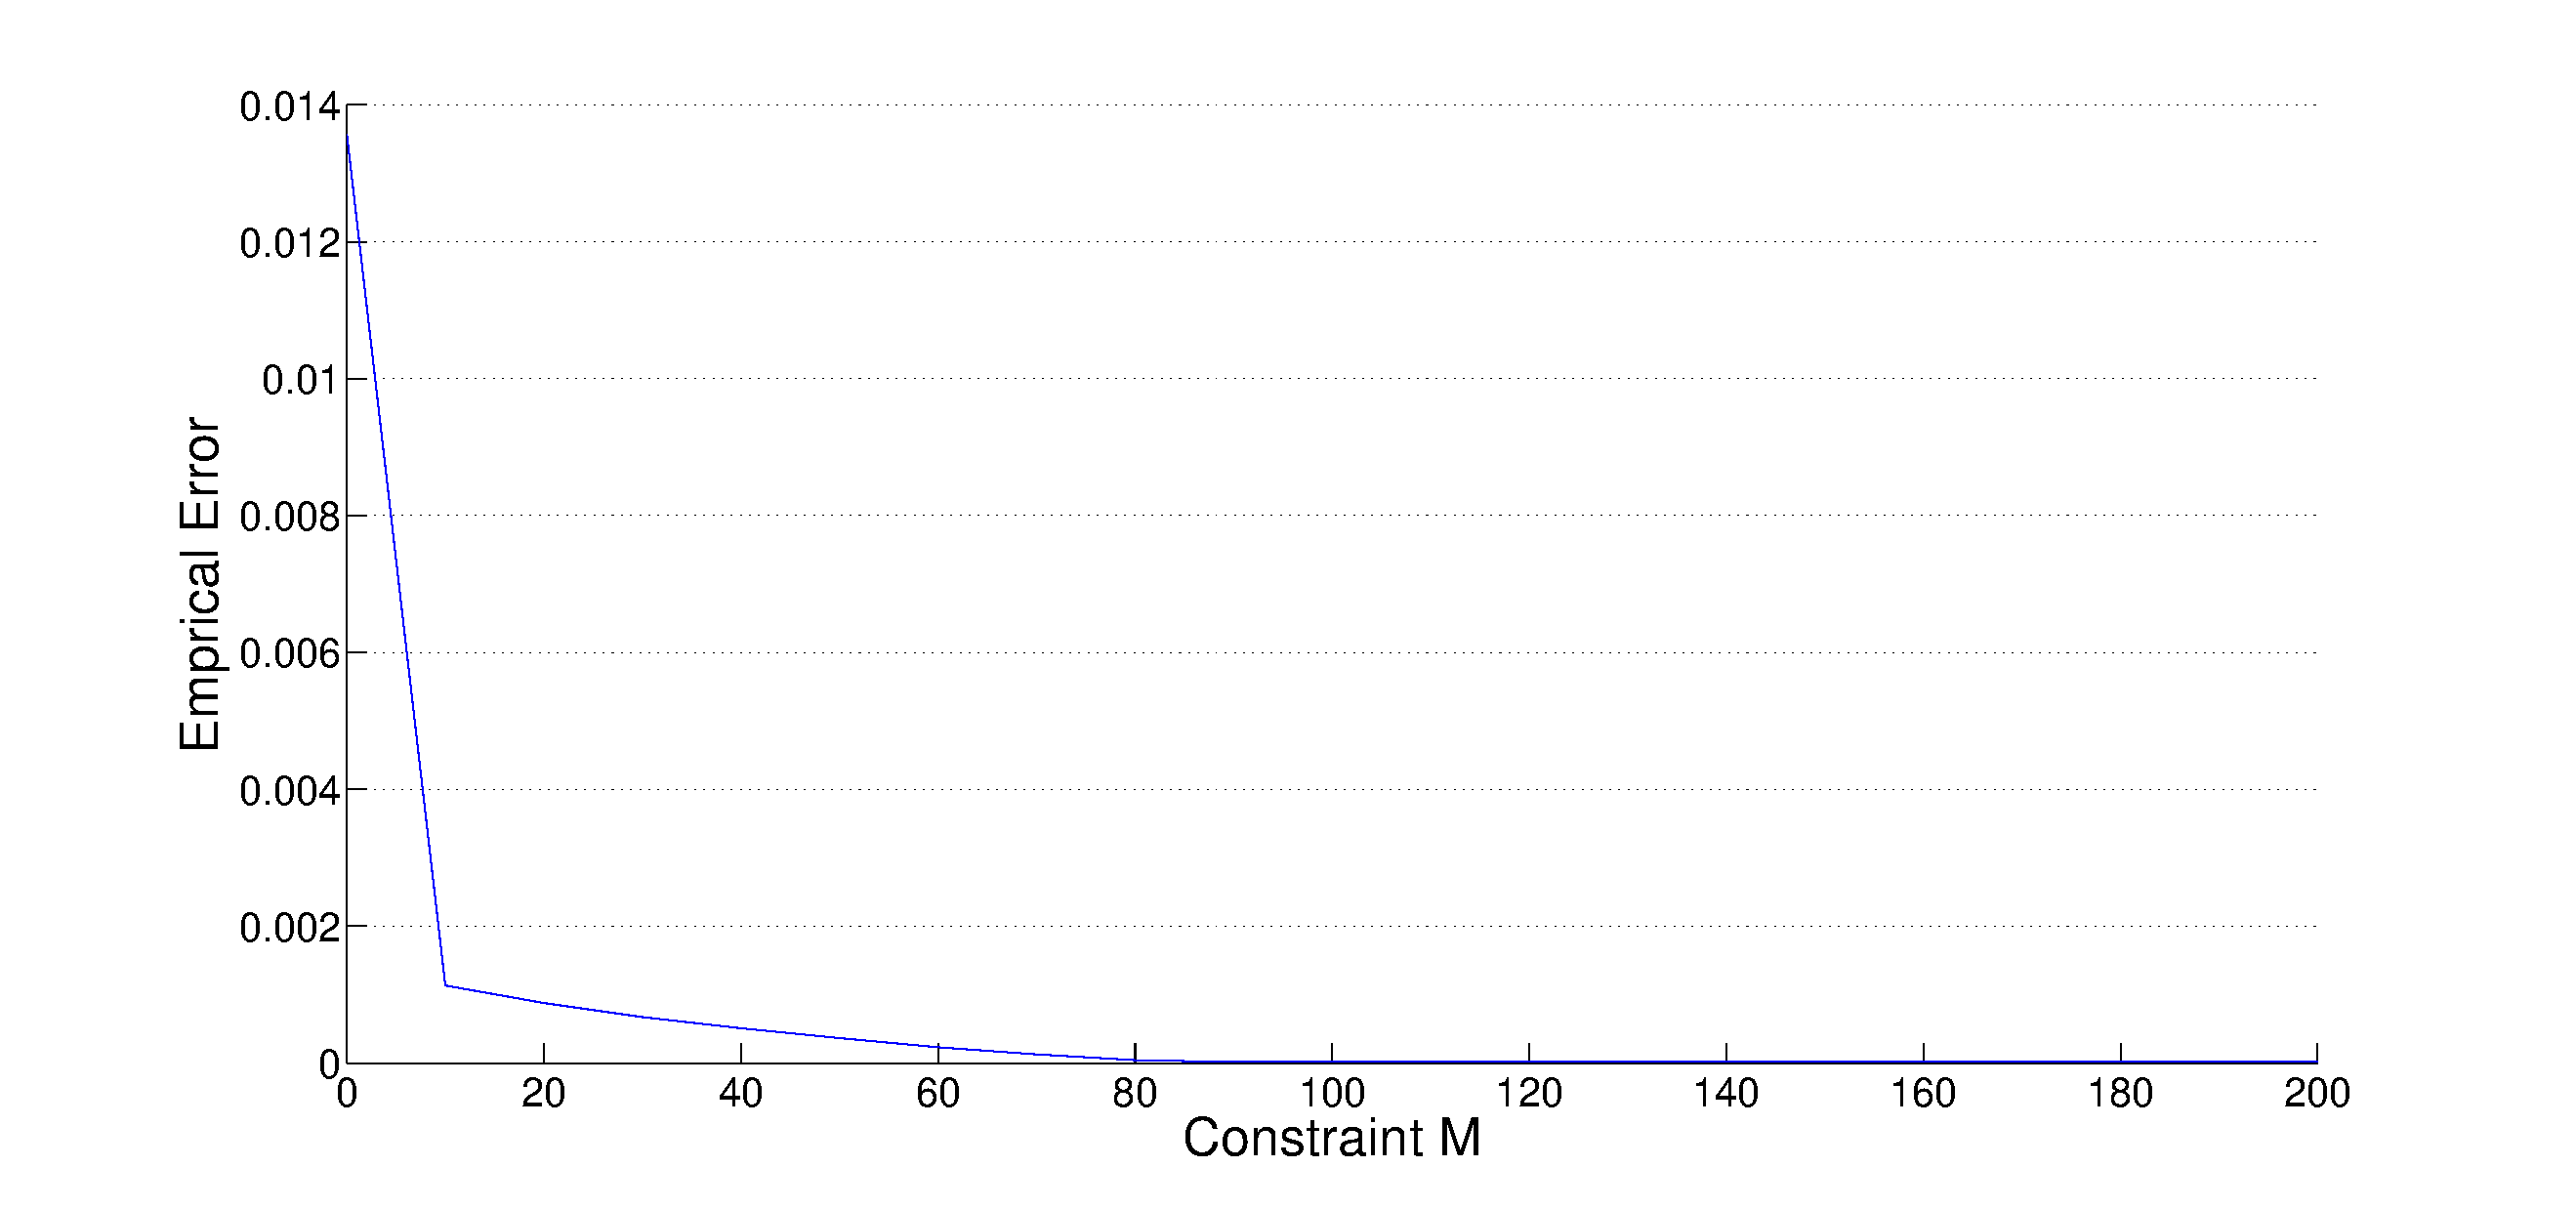
\includegraphics[width=1\textwidth]{figM.eps}
\end{center}
\caption{Values of $\overline{\mathcal{E}}_N$ for fixed $N = 50$ for different values of $M \in [0,200]$.}\label{Mconstr}
\end{minipage}
\end{figure}

In this experiment, the potential $a$ to be retrieved is the truncated Lennard-Jones type interaction kernel of Figure \ref{variableN} and the parameters used in the algorithm are reported in Table \ref{tab:fig3}.

\begin{table}[h]
\begin{center}
\begin{tabular}{ |c|c|c|c|c|c| }
\hline
  $d$ & $L$ & $T$ & $M$ & $N$ & $D(N)$ \\
\hline
\hline
  $2$ & $5$ & $0.5$ & $100$ & $[3,4,\ldots,12]$ & $3N-5$ \\
\hline
\end{tabular}
\end{center}
\vspace{-0.5cm}
\caption{Parameter values for Figure \ref{errorN}} \label{tab:fig3} 
\end{table}

For every value of $N$, we have obtained the minimizer $\widehat{a}_N$ of problem \eqref{problem2} and we have computed the errors $\overline{\mathcal{E}}_N(\widehat{a}_N)$ and $\|a-\widehat{a}_N\|^2_{L_2(\R_+,\rho)}$. The $L_2(\R_+,\rho)$-error multiplied by a factor $\frac{1}{10}$ lies entirely below the curve of $\overline{\mathcal{E}}_N(\widehat{a}_N)$, which let us empirically estimate the value of $c_T$ around that value.

The major issue with this experiment is that the minimization procedure quickly reaches values near machine precision. This causes the inability of the approximation to comply with the increasing number of distances explored by the increasing number of agents, and leads to a resurgence of the $L_2(\R_+,\rho)$-error, which is defined as
\begin{align}
	\|\widehat a-a\|^2_{L_2(\R_+,\rho)} = \frac{1}{T}\int_0^T\int_{\R_+}\bigl|\widehat a(s)-a(s)\bigr|^2 s^2 d\varrho(t)(s) dt.
\end{align}
Hence, rather than seeing a smooth descent to zero for higher values of $N$, due to finite precision a saw-like pattern emerges.
%Hence, rather than seeing a smooth descent to zero for higher values of $N$, a saw-like pattern emerges due to the approximation not being able to cope with the increasing number of distances explored (by the increasing number of agents) in the interval $[0,R]$.

\subsection{Tuning the constraint $M$}

Figure \ref{Mconstr1} shows what happens when we modify the value of $M$ in problem \eqref{problem2}. More specifically, we generate $\mu^N_0$ as explained in Section \ref{numfram} once, and we simulate the system starting from $\mu^N_0$ until time $T$. With the data of this single evolution, we solve problem \eqref{problem2} for several values of $M$, denoting with $\widehat{a}_M$ the minimizer obtained with a specific value of $M$. On the left column of Figure \ref{Mconstr1} we show how the reconstruction $\widehat{a}_M$ gets closer and closer to the true potential $a$ (in white) as $M$ increases, while on the right column we see that the original trajectories (again, in white) used for the inverse problem are approximated better and better by those generated with $\widehat{a}_M$, if we let $M$ grow. Table \ref{tab:figM} reports the values of the parameters of these experiments.

\begin{table}[h]
\begin{center}
\begin{tabular}{ |c|c|c|c|c|c|c| }
\hline
 & $d$ & $L$ & $T$ & $M$ & $N$ & $D(N)$ \\
\hline
\hline
 First row & $2$ & $3$ & $1$ & $2.7 \times [10,15,\ldots,40]$ & $20$ & $60$ \\
\hline
 Second row & $2$ & $3$ & $1$ & $1.25 \times [10,15,\ldots,40]$ & $20$ & $150$ \\
\hline
\end{tabular}
\end{center}
\vspace{-0.5cm}
\caption{Parameter values for Figure \ref{Mconstr1}} \label{tab:figM} 
\end{table}

\begin{figure}[h!]
\begin{center}
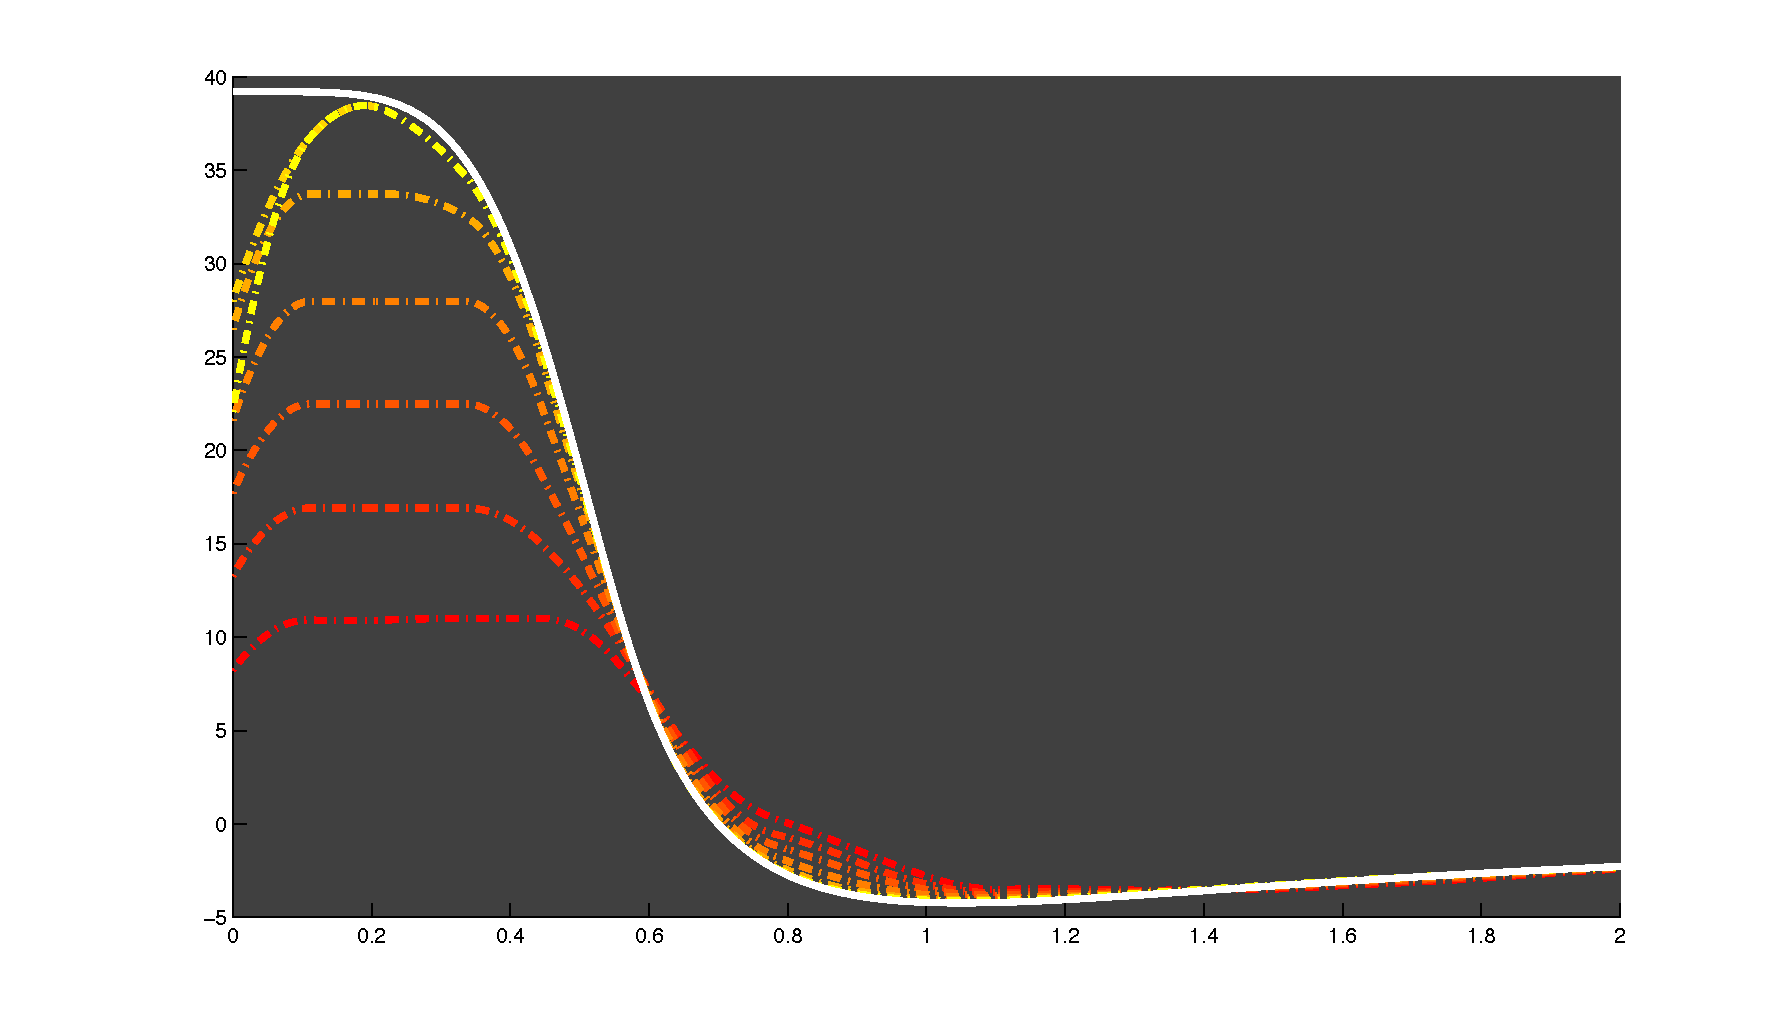
\includegraphics[width=0.53\textwidth]{figPotfun8}
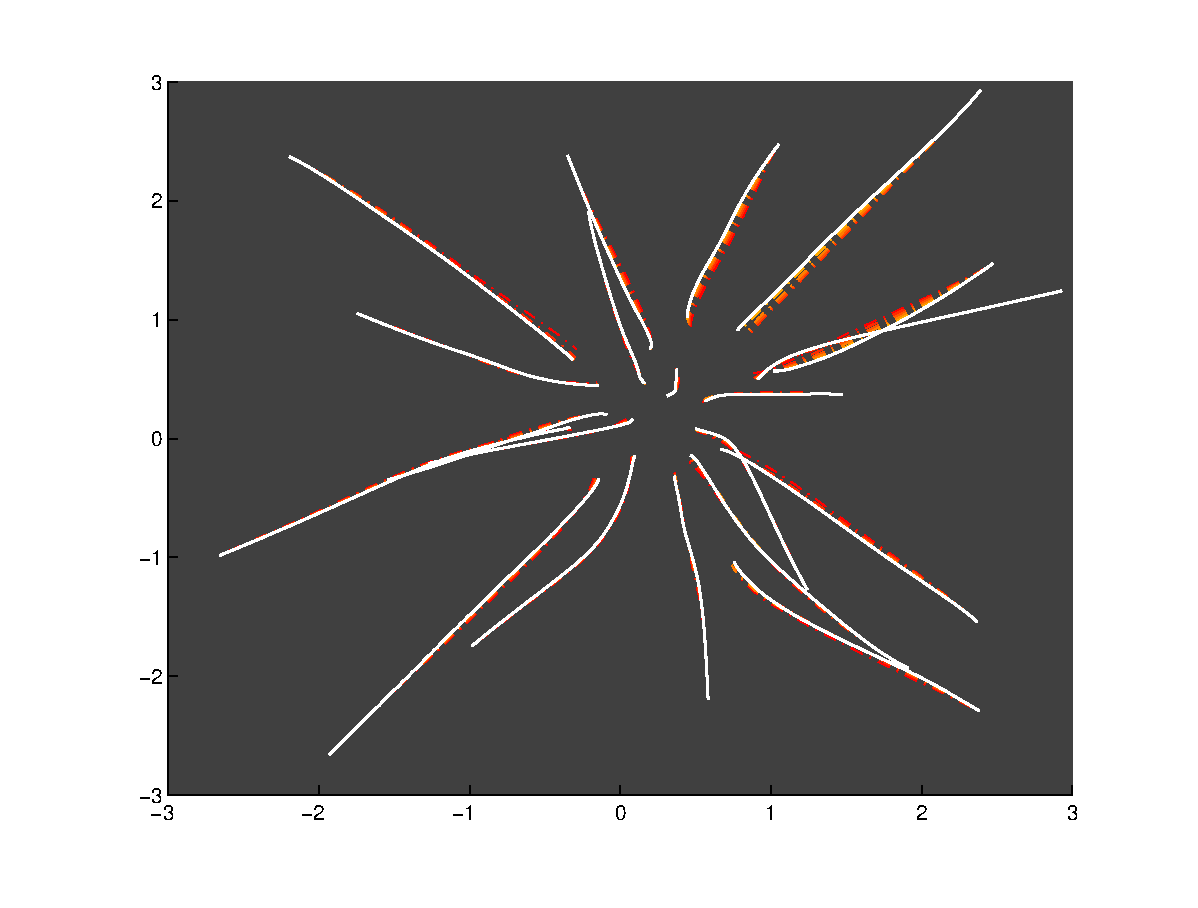
\includegraphics[width=0.37\textwidth]{figTrajfun8}\\
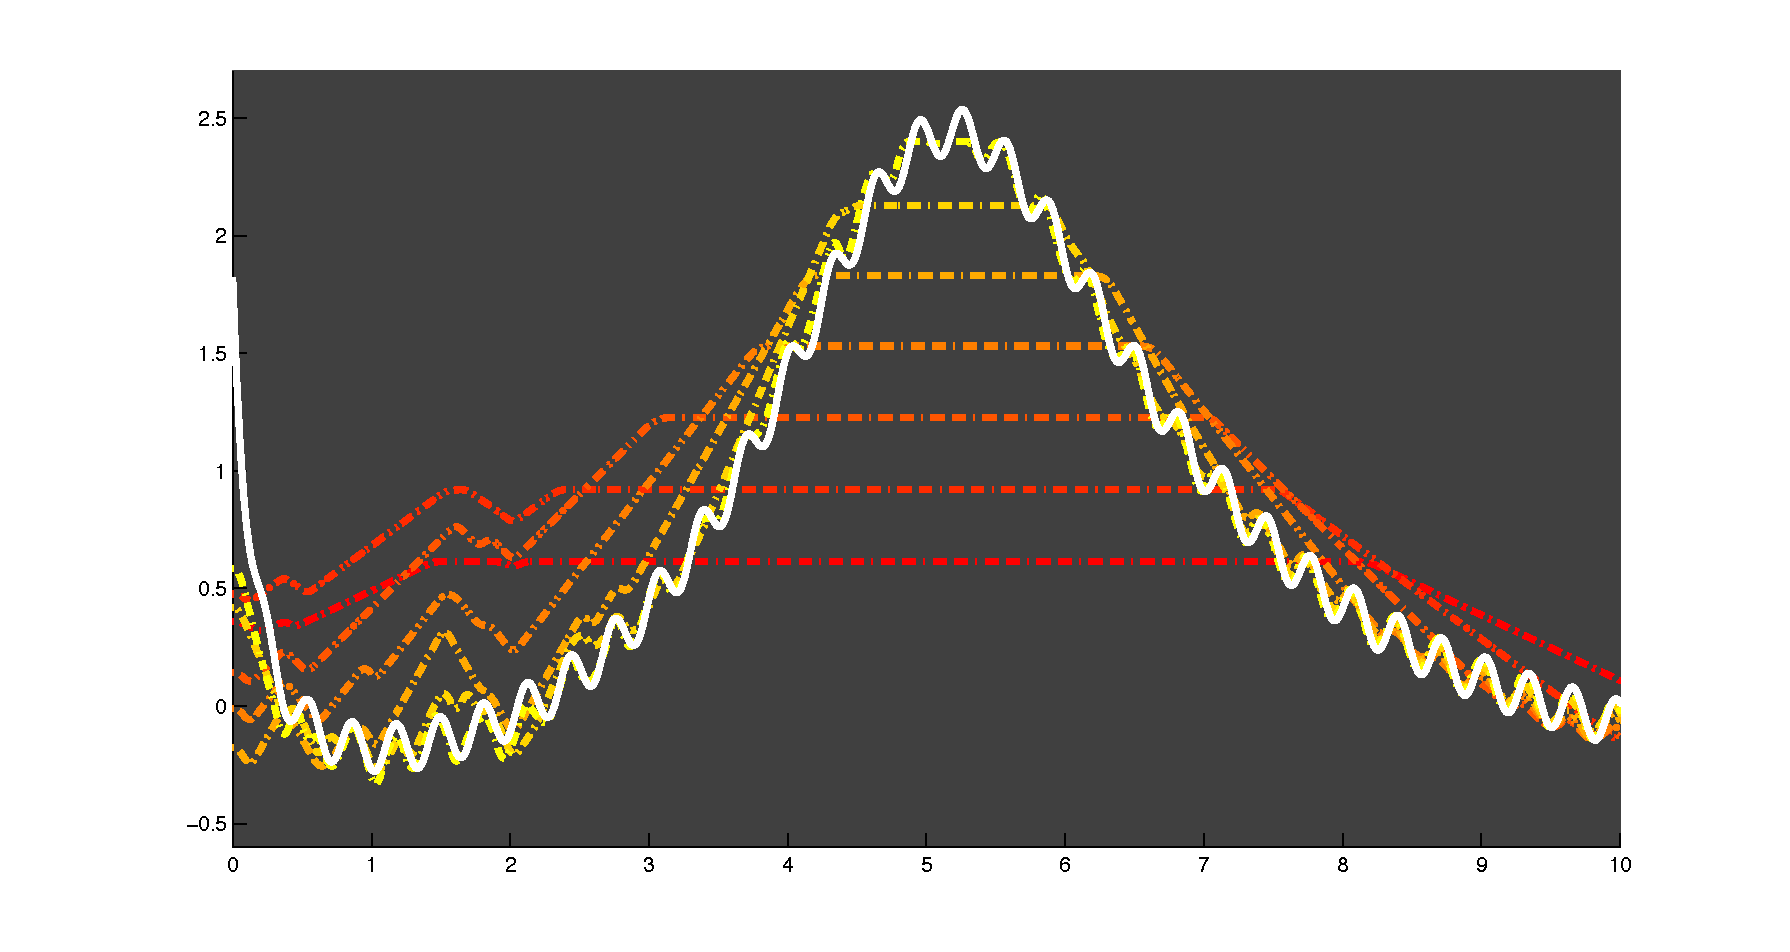
\includegraphics[width=0.53\textwidth]{figPotfun61}
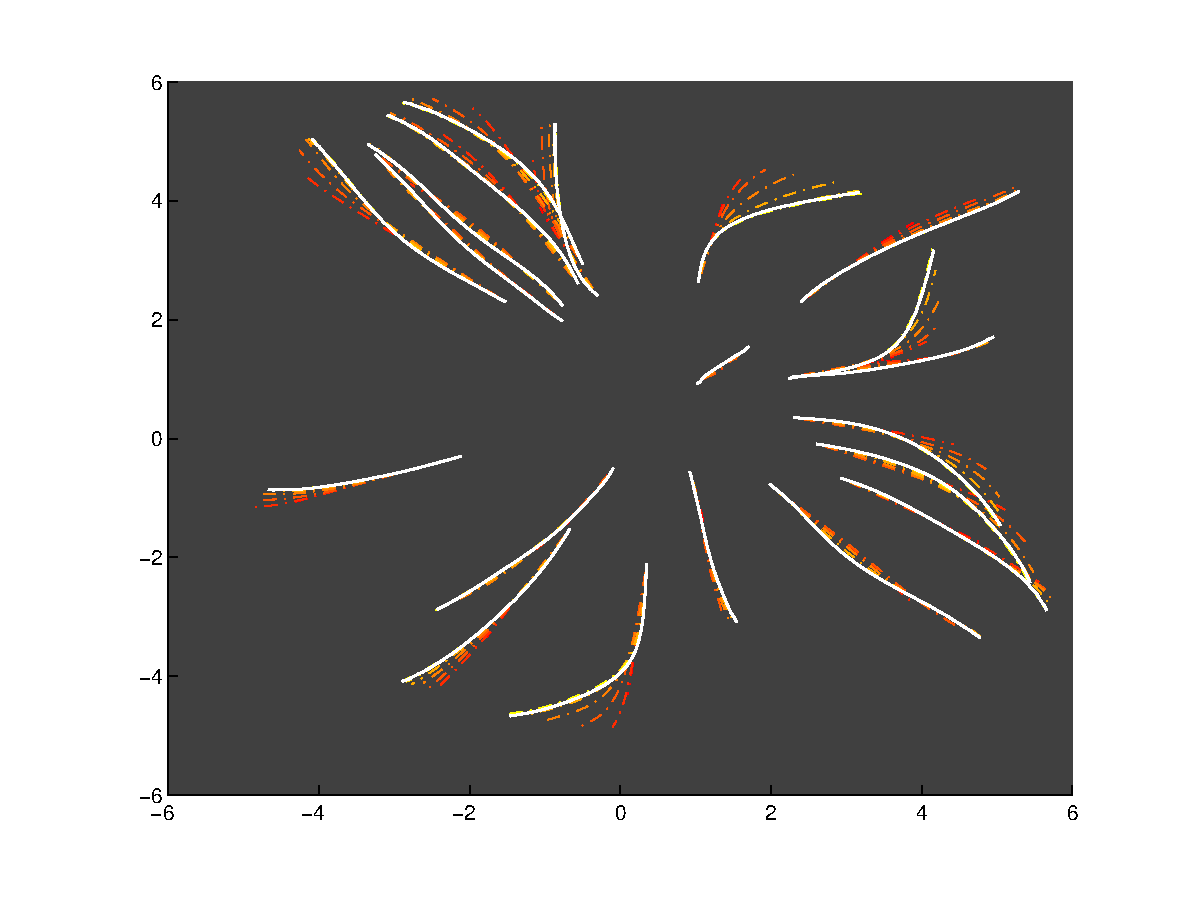
\includegraphics[width=0.37\textwidth]{figTrajfun61}
\end{center}
\caption{Iterative reconstruction of a potential with different values of $M$. On the left column: the true kernel in white and its reconstructions for different $M$; the brighter the curve, the larger the $M$. On the right column: the true trajectories of the agents in white, the trajectories associated to the reconstructed potentials with the same color.}\label{Mconstr1}
\end{figure}

Until now, we have no criteria to sieve those values of $M$ which enable a successful reconstruction of a potential $a \in X$. To carry out such an analysis, we fix all the parameters of our problem as in Table \ref{tab:fig4} and again take $a$ to be the truncated Lennard-Jones type potential of Figure \ref{variableN}. From what we said in the previous section regarding the continuous-time error functional $\mathcal{E}_N$, we can expect two things from the discrete-time one $\overline{\mathcal{E}}_N$ if we keep $N$ fixed:
\begin{itemize}
\item that $\overline{\mathcal{E}}_N(\widehat{a}_M)$ will be decreasing as $M$ increases. This follows from the fact that our constraint in problem \eqref{problem2} is an inequality, therefore the bigger $M$, the larger the class of potential minimizers;
\item that there is a critical value $\overline{M} > 0$ such that $\overline{\mathcal{E}}_N(\widehat{a}_M)$ stabilizes as $M \geq \overline{M}$. Indeed, from the assumption $a \in X$ follows that after you hit $\overline{M} := \|a\|_{L_{\infty}(K)} + \|a'\|_{L_{\infty}(K)}$, the class of potential minimizers should not grow much more.
\end{itemize}

\begin{table}[h]
\begin{center}
\begin{tabular}{ |c|c|c|c|c|c| }
\hline
  $d$ & $L$ & $T$ & $M$ & $N$ & $D(N)$ \\
\hline
\hline
  $2$ & $3$ & $0.5$ & $[0,10,20,\ldots,200]$ & $50$ & $100$ \\
\hline
\end{tabular}
\end{center}
\vspace{-0.5cm}
\caption{Parameter values for Figure \ref{Mconstr}} \label{tab:fig4} 
\end{table}

Figure \ref{Mconstr} document precisely this expected behavior. This actually suggests that an effective strategy to find a sufficiently good constraint $M$ \textit{a posteriori} is to perform an experiment like the one in Figure \ref{Mconstr} and to choose an $M$ after which the curve of $\overline{\mathcal{E}}_N(\widehat{a}_M)$ flattens.

\subsection{Reconstruction with $N$ fixed}

We now explore the possibility of a reconstruction strategy which does not rely on increasing the value of $N$. Indeed, problem \eqref{problem2} can swiftly become unfeasible when $N$ is moderately large, also because the dimension of the invading subspaces $V_N$ increase with $N$ too. A strategy to overcome this limitation could be to consider, for a fixed $N$, several discrete initial data $(\mu^N_{0,i})_{i = 1}^{\Theta}$ all independently drawn from the same distribution $\mu_0$ (in our case, the $d$-dimensional cube $[-L,L]^d$). For every $i = 1,\ldots,\Theta$, we simulate the system until time $T$ and, with the trajectories we obtain, we solve problem \eqref{problem2}. At the end of this procedure, we have a family of reconstructed potentials $(\widehat{a}_{N,i})_{i = 1}^{\Theta}$, all approximating the same true kernel $a$. Averaging these potentials, we obtain a functional
\begin{align*}
\widehat{a}_N(r) = \frac{1}{\Theta} \sum^{\Theta}_{i = 1}\widehat{a}_{N,i}(r), \quad \text{ for every } r \in [0,R],
\end{align*}
which we claim to be a good approximation to the true kernel $a$. To motivate this claim, we report the outcome of an experiment whose data can be found in Table \ref{tab:fig5}.

\begin{table}[h]
\begin{center}
\begin{tabular}{ |c|c|c|c|c|c|c| }
\hline
  $d$ & $L$ & $T$ & $M$ & $N$ & $D(N)$ & $\Theta$ \\
\hline
\hline
  $2$ & $2$ & $0.5$ & $1000$ & $50$ & $150$ & 5  \\
\hline
\end{tabular}
\end{center}
\vspace{-0.5cm}
\caption{Parameter values for Figure \ref{fixedN}} \label{tab:fig5} 
\end{table}

Figure \ref{fixedN} shows the true potential $a$ and the averaged reconstruction $\widehat{a}_N$. The black-dotted lines corresponds to the 95\% confidence interval obtained from the averaged data.

\begin{figure}[h!]
\begin{center}
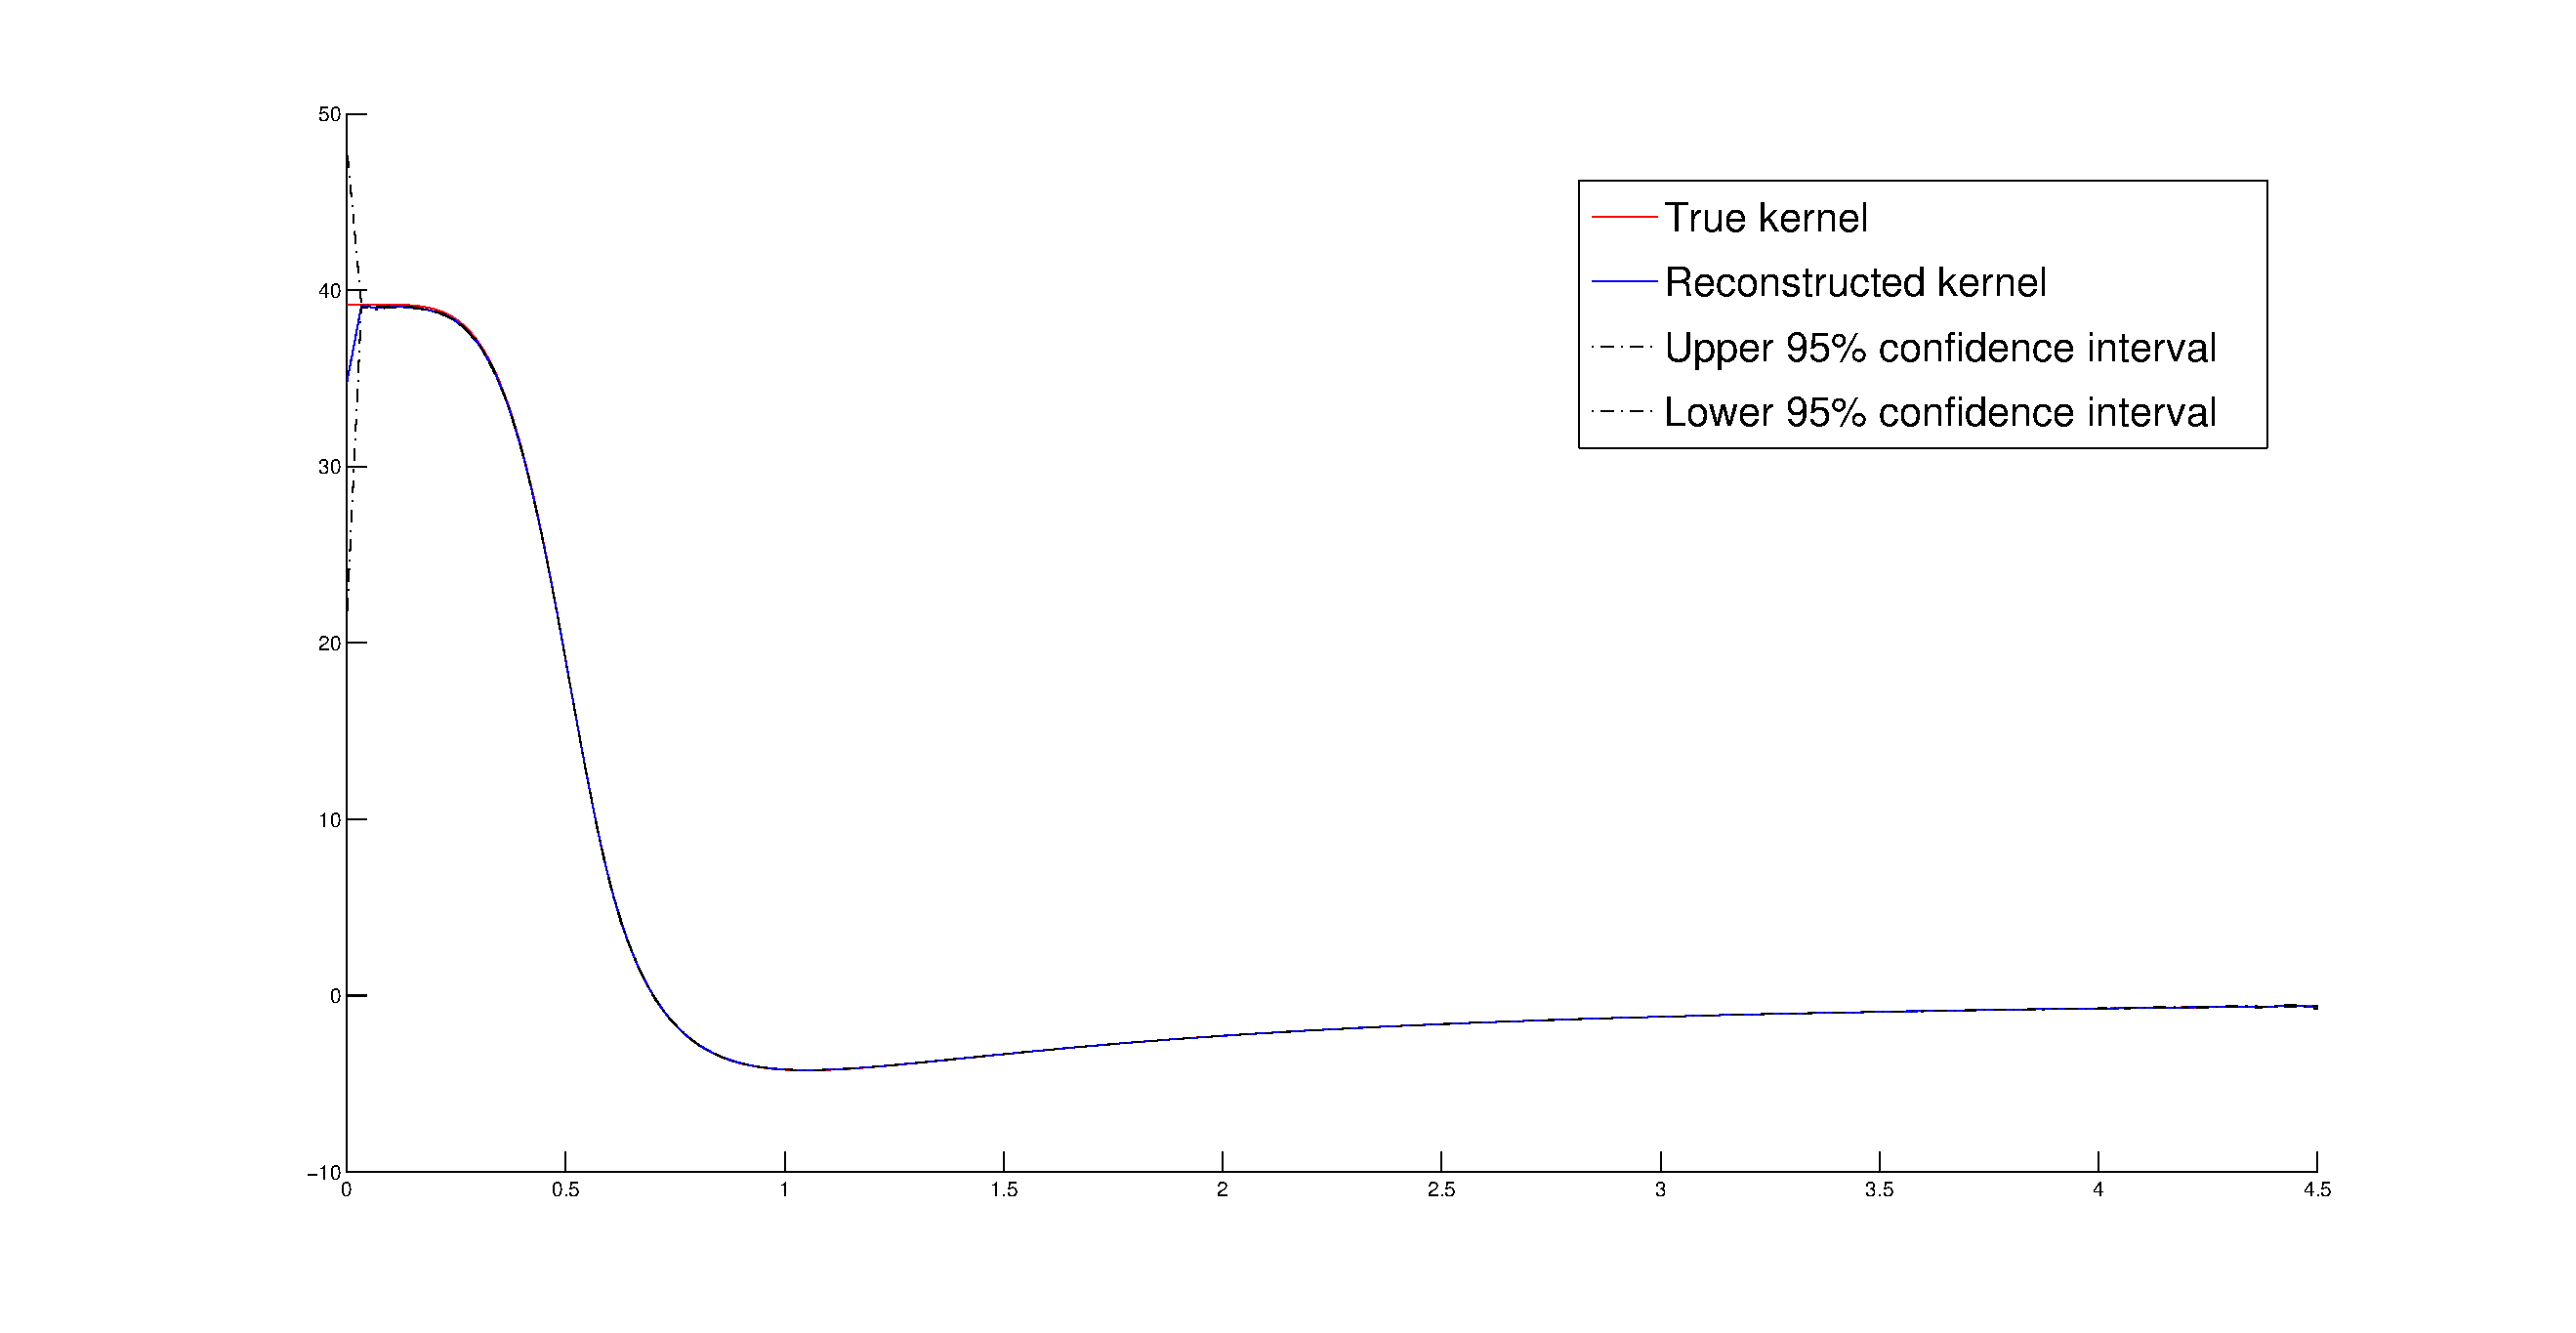
\includegraphics[width=\textwidth]{figNfisso.eps}
\end{center}
\caption{Reconstruction of $a$ obtained by averaging 5 solutions of the minimization of $\mathcal{E}_N$ for $N = 50$. In red: the unknown kernel. In blue: the average of reconstructions. In black: 95\% confidence interval.}\label{fixedN}
\end{figure}


\section*{Acknowledgement}

Mattia Bongini, Massimo Fornasier, and Markus Hansen acknowledge the financial support of the ERC-Starting Grant (European Research Council, 306274) “High-Dimensional Sparse Optimal Control” (HDSPCONTR). Mauro Maggioni acknowledges the support of ONR-N00014-12-1-0601 and NSF-ATD/DMS-12-22567. The authors acknowledge the hospitality and the financial support of the University of Bonn and the Hausdorff Center for Mathematics during the Hausdorff Trimester Program ``Mathematics of Signal Processing" for the final preparation of this work.


\section{Appendix}

We show now the proof of Proposition \ref{pr:exist} which states the existence of solutions for \eqref{eq:contdyn}. We will need the following Lemma,
which may be proved with proofs similar to those for \cite[Lemma 6.7]{MFOC} and \cite[Lemma 4.7]{CanCarRos10}

\begin{lemma}\label{p-lipkernel}
Let $a \in X$ and let $\mu:[0,T] \rightarrow \mathcal{P}_c(\R^d)$ and $\nu: [0,T] \to \mathcal{P}_c(\R^d)$ be two continuous maps with respect to $\W_1$ satisfying
\begin{align}\label{eq:bsupp}
\supp(\mu(t)) \cup \supp(\nu(t)) \subseteq B(0,R),
\end{align}
for every $t \in [0,T]$, for some $R > 0$. Then for every $r > 0$ there exists a constant $L_{a,r,R}$ such that
\begin{align}\label{eq:inftynormW1}
\|\Fun{a} * \mu(t) - \Fun{a} * \nu(t)\|_{L_{\infty}(B(0,r))} \leq L_{a,r,R} \W_1(\mu(t),\nu(t))
\end{align}
for every $t \in [0,T]$.
\end{lemma}


\begin{proof}[Proof of Proposition \ref{pr:exist}]
Let us define the quantity $\mathcal X_N(t) := \max_{i=1,\dots,N} |x_i^N(t)|$. By integration of \eqref{eq:discr1} we obtain
\begin{eqnarray*}
 |x_i^N(t)| &\leq& |x^N_{0,i}| + \int_0^t (\Fun{a} * \mu^N(s))(x_i^N)| ds \\
&\leq&  |x^N_{0,i}| + \int_0^t\frac{1}{N} \sum_{j=1}^N |a(|x_i-x_j|)||x_j-x_i| ds \\
&\leq&  |x^N_{0,i}| + \|a\|_{L_{\infty}(\R_+)} \int_0^t\frac{1}{N} \sum_{j=1}^N( |x_j| + | x_i| )ds,
\end{eqnarray*}
implying
$$
\mathcal X_N(t) \leq \mathcal X_N(0) + 2  \|a\|_{L_{\infty}(\R_+)} \int_0^t \mathcal X_N(s) ds. 
$$
Hence, Gronwall's Lemma and the hypothesis $x^{N}_{0,i} \in \supp(\mu_0)$ for every $N \in \N$ and $i = 1, \ldots, N$, imply that
\begin{align*}
\mathcal X_N(t) \leq \mathcal X_N(0) e^{2 \|a\|_{L_{\infty}(\R_+)} t} \leq C_0 e^{2 \|a\|_{L_{\infty}(\R_+)} t} \text{ for a.e. } t \in [0,T],
\end{align*}
for some uniform constant $C_0$ depending only on $\mu_0$. Therefore, the support of the empirical measure $\mu^N(\cdot)$ is bounded uniformly in $N$ in a ball $B(0,R) \subset \R^d$, where
\begin{align}\label{Rest}
R =  C_0 e^{2 \|a\|_{L_{\infty}(\R_+)} T}.
\end{align}
Now, notice that from \eqref{dualwass} it follows
$$
\mathcal W_1(\mu^N(t), \mu^N(s)) \leq \frac{1}{N} \sum_{i=1}^N | x_i^N(t) - x_i^N(s)| ,
$$
and the local Liptschitz contiunuity of $\mu^N(t)$ follows from the one of $x_i^N(t)$: indeed  $|x^N_i(t)| \leq R$ for a.e. $t \in [0,T]$, for all $N \in N$ and $i = 1, \ldots, N$, and Lemma \ref{p-estkernel} yields
\begin{align*}
|\dot{x}^N_i(t)| &= |(\Fun{a}*\mu^N(t))(x^N_i(t))| \\
&\leq \|a\|_{L_{\infty}(\R_+)} \left( |x^N_i(t)| + \frac{1}{N}\sum^N_{j = 1}|x^N_j(t)|\right) \\
&\leq 2R\|a\|_{L_{\infty}(\R_+)}.
\end{align*}
Hence, the sequence $(\mu^N)_{N \in \N} \subset \mathcal{C}^0([0,T],\mathcal{P}_1(B(0,R)))$ is equicontinuous, because equi-Lipschitz continuous, and equibounded in the complete metric space $(\mathcal{P}_1(B(0,R)),\W_1)$.
Therefore, we can apply the Ascoli-Arzel\'{a} Theorem for functions with values in a metric space (see for instance, \cite[Chapter 7, Theorem 18]{KelleyTop}) to infer the existence of a subsequence $(\mu^{N_k})_{k \in \N}$ of $(\mu^N)_{N \in \N}$ such that
\begin{align}\label{eq:unifconv}
\lim_{k \rightarrow \infty}\W_1(\mu^{N_k}(t),\mu(t)) = 0 \quad \text{ uniformly for a.e. } t \in [0,T],
\end{align}
for some $\mu \in \mathcal{C}^0([0,T],\mathcal{P}_1(B(0,R)))$ with Lipschitz constant bounded by $2R\|a\|_{L_{\infty}(\R_+)}$. The hypothesis $\lim_{N\rightarrow\infty}\W_1(\mu^N_0,\mu_0) = 0$ now obviously implies $\mu(0) = \mu_0$. In particular it holds
\begin{equation}\label{initialdatum}
\lim_{k\to \infty} \langle \varphi, \mu^N(t) - \mu^N(0) \rangle  =  \langle \varphi, \mu(t) - \mu_0 \rangle
\end{equation}
for all $\varphi \in \mathcal{C}^1_c(\R^d;\R)$.


We are now left with verifying that this curve $\mu$ is a solution of \eqref{eq:contdyn}. For all $t \in [0,T]$ and for all $\varphi \in \mathcal{C}^1_c(\R^d;\R)$, it holds
\begin{align*}
\frac{d}{dt}\langle \varphi, \mu^N(t) \rangle = \frac{1}{N}\frac{d}{dt} \sum^N_{i = 1} \varphi(x^N_i(t)) = \frac{1}{N} \sum^N_{i = 1} \nabla\varphi(x^N_i(t)) \cdot \dot{x}_i^N(t).
\end{align*}
By directly applying the substitution $\dot{x}_i^N(t) = (\Fun{a}*\mu^N(t))(x^N_i(t))$, we have
\begin{align*}
\langle \varphi, \mu^N(t) - \mu^N(0) \rangle = \int^t_0 \left[ \int_{\R^d}\nabla \varphi(x) \cdot (\Fun{a}*\mu^N(s))(x) d\mu^N(s)(x) \right] ds.
\end{align*}
By Lemma \ref{p-lipkernel}, the inequality \eqref{eq:inftynormW1}, and the compact support of $\varphi \in \mathcal{C}^1_c(\R^d;\R)$, it follows
\begin{align*}
\lim_{N \rightarrow \infty} \|\nabla\varphi \cdot (\Fun{a}*\mu^N(t) - \Fun{a}*\mu(t))\|_{L_{\infty}(\R^d)} = 0 \quad \text{ uniformly for a.e. } t \in [0,T].
\end{align*}
If we denote with $\mathcal L_1\llcorner_{[0,t]}$ the Lebesgue measure on the time interval $[0,t]$, since the product measures $\frac{1}{t} \mu^{N}(s) \times \mathcal L_1\llcorner_{[0,t]}$ converge in $\mathcal P_1([0,t] \times \mathbb R^{d})$ to $\frac{1}{t} \mu(s) \times \mathcal L_1\llcorner_{[0,t]}$, we finally get from the dominated convergence theorem that
\begin{align}
\lim_{N \to \infty} \int_0^{t} \int_{\mathbb R^{d}} \nabla \phi(x) \cdot (\Fun{a}*&\mu^N(s))(x) d\mu^N(s)(x) ds  \nonumber \\
&=  \int_0^{t} \int_{\mathbb R^{d}} \nabla \phi(x) \cdot (\Fun{a}*\mu(s))(x) d \mu(s)(x) ds, \label{limitmf}.
\end{align}
The statement now follows from combination of \eqref{initialdatum} and \eqref{limitmf}.  
\end{proof}



\begin{proof}[Proof of Lemma \ref{rhosc}] As a first step we show that for every given sequence $(t_n)_{n \in \N}$ converging to $t\in [0,T]$ we have the weak
	convergence $\varrho(t_n)\rightharpoonup\varrho(t)$ for $n \rightarrow \infty$. 
	%For this, in turn we first prove the weak convergence of the product measure $\mu(t_n)\otimes\mu(t_n)\rightharpoonup\mu(t)\otimes\mu(t)$.
	We first note that $\mu(t_n)\otimes\mu(t_n)\rightharpoonup\mu(t)\otimes\mu(t)$, since $\mu(t_n)\rightharpoonup\mu(t)$ because of the continuity of $\mu(t)$ in the Wasserstein metric $\W_1$.	
%	A well-known property of the space $\mathcal{C}(\R^d\times\R^d)$ is that it coincides with the inductive tensor product
%	$\mathcal{C}(\R^d)\otimes_\varepsilon \mathcal{C}(\R^d)$. In particular, functions of the form $h=\sum_{j=1}^J f_j\otimes g_j$ with
%	$f_j,g_j\in \mathcal{C}(\R^d)$, for $j=1,\ldots,J$ and $J\in\N$, are a dense subspace of $\mathcal{C}(\R^{2d})$. Hence, to prove the weak
%	convergence of measures on $\R^{2d}$, we can restrict the proof to functions of this form. Due to linearity of
%	integrals, this can be further reduced to simple tensor products of the form $h=f\otimes g$.
%	
%	For such tensor products we can directly apply Fubini's Theorem and the weak convergence
%	$\mu(t_n)\rightharpoonup\mu(t)$ (which is a consequence of the continuity of $\mu$ w.r.t. the
%	Wasserstein metric $\W_1$), and find
%	\[
%		\int_{\R^{2d}}f\otimes g\, d(\mu(t_n)\otimes\mu(t_n))
%			=\int_{\R^d}f d\mu(t_n)\cdot\int_{\R^d}g d\mu(t_n)
%			\stackrel{n\rightarrow\infty}{\longrightarrow}\int_{\R^d}f d\mu(t)\cdot\int_{\R^d}g d\mu(t).
%	\]
	This implies the claimed weak convergence $\varrho(t_n)\rightharpoonup\varrho(t)$, since for any
	function $f\in \mathcal{C}(\R_+)$, it holds $f\circ d\in\mathcal{C}(\R^d\times\R^d)$, and hence
	\begin{align*}
		\int_{\R_+}f\,d\varrho(t_n)
			&=\int_{\R^{2d}}(f\circ d)(x,y)d(\mu(t_n)\otimes\mu(t_n))(x,y)\\
			&\stackrel{n\rightarrow\infty}{\longrightarrow}
				\int_{\R^{2d}}(f\circ d)(x,y)d(\mu(t)\otimes\mu(t))(x,y)
			=\int_{\R_+}f\,d\varrho(t).
	\end{align*}
	The claim now follows from general results for weakly* convergent sequences of Radon measures, see e.g. \cite[Proposition 1.62]{AFP00}.
\end{proof}


\begin{proof}[Proof of lemma \ref{lemma-AC-1}]
Both $\mu_0$ and $\mu(t)$ are supported in $B(0,R)$, with $R$ as in \eqref{Rest}. The measure $\mu(t)$ is the pushforward of $\mu_0$ under the locally bi-Lipschitz map $\ct^\mu_t$, see Proposition \ref{p-transportlip}. Since $\ct^\mu_t$ has Lipschitz inverse on $B(0,R)$, this inverse maps $\cl_d$-null sets to $\cl_d$-null sets, so $\mu_0$-null sets are not only $\cl_d$-null sets by assumption, but are also $\mu(t)$-null sets.
\end{proof}

\begin{proof}[Proof of Lemma \ref{le-abs}]
	Fix $t\in [0,T]$. By Lemma \ref{lemma-AC-1} we already know that $\mu(t)$ is absolutely continuous w.r.t.
	$\cl_d$, and so $\mu(t)\otimes\mu(t)$ is absolutely continuous w.r.t. $\cl_{2d}$. It hence
	remains to show that $\cl_{2d}$ is absolutely continuous w.r.t. $\cl_1\llcorner_{\R_+}$, where $d$ is the distance function,
	but this follows easily by observing that $d^{-1}(A)=0$ for every $\cl_1\llcorner_{\R_+}$-null set $A$, and an application of Fubini's theorem.	
%	Let $A\subset\R_+$ be a Lebesgue null-set, and put $B=d^{-1}(A)\subset\R^{2d}$. Moreover, we denote by
%	$B_x=\{y\in\R^d:|x-y|\in A\}$. Then clearly $B_{x+z}=z+B_x$. Moreover, using Fubini's Theorem we obtain
%	\begin{align*}
%		\cl_{2d}(B)=\int_{\R^d}\cl_d(B_x)d\cl_d(x)\,.
%	\end{align*}
%	It thus remains to show that $\cl_d(B_x)=0$ for one single $x\in\R^d$ (and thus for all, due to translation invariance of $\cl_d$).
%	However, to calculate $\cl_d(B_0)$, we can pass to polar coordinates, and once again using Fubini's Theorem
%	we obtain
%	\begin{align*}
%		\cl_d(B_x)=\int_{\R^d}\chi_{B_0}(y)d\cl_d(y)
%			=\int_{S^d}\int_{\R_+}\chi_A(r)dr d\omega=\Omega_d\cl_1(A)=0\,,
%	\end{align*}
%	where $\Omega_d$ is the surface measure of the unit sphere $S_d$. This proves the absolute continuity of
%	$\varrho(t)$, since
%	\begin{align*}
%		\cl_1(A)=0\Longrightarrow\cl_{2d}(d^{-1}(A))
%			\Longrightarrow (\mu(t)\otimes\mu(t))(d^{-1}(A))=0\iff\varrho(t)(A)=0\,.
%	\end{align*}
	The absolute continuity of $\prerho$ now follows immediately from the one of $\varrho(t)$ for every $t$ and its
	definition as an integral average \eqref{eq-rho-4}.
\end{proof}


\begin{proof}[Proof of Lemma \ref{rhocompact}]
We have
\begin{align*}
\begin{split}
\prerho(\R_+)&= \frac{1}{T}\int_0^T \varrho(t)(\R_+)dt 
%&= \frac{1}{T}\int_0^T (\mu(t) \otimes \mu(t))(d^{-1}(\R_+))dt \\
= \frac{1}{T}\int_0^T \int_{\R^d \times \R^d} |x - y| d\mu(t)(x) d \mu(t)(y)dt
<+\infty,
\end{split}
\end{align*}
since the distance function is continuous and the support of $\mu$ is uniformly bounded in time. This shows that $\prerho$ is bounded.
Since the supports of the measures $\varrho(t)$ are the subsets of
$K=\{|x-y|:x,y\in B(0,R)\} = [0,2R]$, where $R$ is given by \eqref{Rest}, by construction we also have $\supp \prerho\subseteq K$.
\end{proof}


\begin{proof}[Proof of Proposition \ref{p:randomcoercivity}]
By assumption $\mathbf K$ has independent Gaussian rows, each with variance $\sigma^2I_N$. %(a random vector $Z$ is called sub-Gaussian with sub-Gaussian norm $\sigma$ if for every $t>1$ and every $\theta$ with norm $1$, $\mathbb{P}( |\langle Z,\theta\rangle| > t) \le 2 e^{-t^2/\sigma^2}$). 
Since the bounds we wish to obtain, and our estimates below, are scale invariant, we may, and will, assume $\sigma=1$. Also, we have fixed a certain time $t_0$, which will be omitted from the notation.
Let $\mathbf{X}_i\in\mathbb{R}^{N\times d}$ be the matrix whose $j$-th row is the vector $\frac{x_i-x_j}{|x_i-x_j|}\in\mathbb{R}^d$, and let $\mathbf{K}(i,:)\in\mathbb{R}^N$ be the $i$-th row of $\mathbf{K}$. The coercivity inequality \eqref{e:coercivitydiscrete} may be re-written as:
\begin{align}
\frac 1N\sum_{i=1}^N\left|\frac1N\mathbf{K}(i,:)\mathbf{X}_i\right|^2\ge\frac{c'_t}{N^2}\|\mathbf{K}\|^2_{\mathbb{F}}\,.
\label{e:coermatrix}
\end{align}
We have
\begin{align*}
\mathbb{E}\left[|\mathbf{K}(i,:)\mathbf{X}_i|^2\right]
&=\sum_{l=1}^d\sum_{j,j'=1}^N\mathbb{E}\left[\mathcal{K}(|x_i-x_j|)\mathcal{K}(|x_i-x_{j'}|)|\right] \left(\frac{x_i-x_j}{|x_i-x_j|}\right)_l \left(\frac{x_i-x_{j'}}{|x_i-x_{j'}|}\right)_l\\
&=\sum_{j=1}^N \mathbb{E}\left[\mathcal{K}(|x_i-x_j|)^2\right] \sum_{l=1}^d\left(\frac{x_i-x_j}{|x_i-x_j|}\right)^2_l = \sum_{j=1}^N \mathbb{E}\left[\mathcal{K}(|x_i-x_j|)^2\right]=N\\
%&= \sum_{j=1}^N |\mathbf{X}_i(j,:)|^2 = \| \mathbf{X}_i\|^2_{\mathbb{F}}=N\,,
\end{align*}
where we used independence, %in the second step we used standard properties of random projections (or inner products) against Gaussian vectors \cite{Vershynin:NARMT}, 
and in the last step we used the fact that every row of $\mathbf{X}_i$ is a unit vector. By concentration arguments (e.g. \cite{Vershynin:NARMT}) one readily obtains that with high probability
\begin{align*}
\frac 1N\sum_{i=1}^N\left|\frac1N\mathbf{K}(i,:)\mathbf{X}_i\right|^2\ge\frac CN\,.
\end{align*}
One the other hand, since $\mathbb{E}[||\mathbf{K}||^2_{\mathbb{F}}]\le CN^2$ by standard random matrix theory results (e.g. \cite{Vershynin:NARMT}), and in fact not just in expectation but also with high probability, the right hand side of \eqref{e:coermatrix} is bounded by $c'_{t_0}C$ from above. Choosing $c'_{t_0}$ small enough (and at least as small as $O(1/N)$, as a function of $N$), we obtain \eqref{e:coermatrix} with high-probability.

For the second case, we proceed exactly as above, and note that in this case
\begin{align*}
\mathbb{E}\left[|\mathbf{K}(i,:)\mathbf{X}_i|^2\right] = \sum_{j=1}^N |x_i-x_j|^{-\alpha}\,.
\end{align*}
Continuing as above, we obtain that with high probability
$$
\frac 1N\sum_{i=1}^N\left|\frac1N\mathbf{K}(i,:)\mathbf{X}_i\right|^2\ge \frac1N\sum_{i=1}^N\frac CN\sum_{j=1}^N |x_i-x_j|^{-2\alpha}\ge C \,,
$$
which implies the claim.
\end{proof}




%\section{Appendix}
%
% Although  similar results on the limit relationship between ODE systems of the type \eqref{eq:discrdyn} and their mean-field equations \eqref{eq:contdyn}
%appear in different forms in other papers, see, e.g., \cite{AGS,CanCarRos10,13-Carrillo-Choi-Hauray-MFL,MFOC}, in this Appendix we collect them for our specific setting in a nutshell for the sake of being self-contained and for the convenience of those readers less familiar with these properties of evolutive systems.
%
%
%
%%\subsection{Standard results on existence and uniqueness for ODE}\label{ap00}
%%
%%For the reader's convenience and for the sake of a self-contained presentation, we start by briefly recalling some general, well-known results about solutions to Carath{\'e}odory differential equations. We fix a domain $\Omega \subset \R^d$, a Carath{\'e}odory function $g\colon[0,T]\times \Omega \to \R^d$, i.e. the function $g$ is continuous in $y$ and measurable in $t$, and $0<\tau \le T$. A function $y\colon [0,\tau]\to \Omega$ is called a solution of the Carath{\'e}odory differential equation
%%\begin{equation}\label{cara}
%%\dot y(t)=g(t, y(t))
%%\end{equation}
%%on $[0,\tau]$ if and only if $y$ is absolutely continuous and \eqref{cara} is satisfied a.e.\ in $[0,\tau]$.
%%The following well-known local existence result holds, see \cite[Chapter 1, Theorem 1]{Fil} .
%%
%%
%%\begin{theorem}\label{cara-local}
%%Fix $T > 0$ and $y_0 \in \R^d$. Suppose that there exists a compact subset $\Omega$ of $\R^d$ such that $y_0 \in \textup{int}(\Omega)$ and there exists $m_{\Omega} \in L_1([0,T])$ for which it holds
%%%Consider an interval $[0,T]$ on the real line, a compact subset $K$ of $\R^n$, and a Carath{\'e}odory function $g\colon[0,T]\times \R^n \to \R^n$. If there exists a function $m \in L_1((0,T))$ such that
%%\begin{align}\label{l1}
%%|g(t,y)|\le m_{\Omega}(t),
%%\end{align}
%%for a.e.\ $t \in [0,T]$ and for all $y \in \Omega$. Then there exists a $\tau > 0$ and a solution $y(t)$ of \eqref{cara} defined on the interval $[0,\tau]$ which satisfies $y(0)=y_0$. 
%%\end{theorem}
%%
%%The result can be extended to a global existence as follows.
%%
%%\begin{theorem}\label{cara-global}
%%Consider an interval $[0,T]$  on the real line and a  Carath{\'e}odory function $g\colon[0,T]\times \R^d \to \R^d$.
%%Assume that there exists a constant $C > 0$ such that the function $g$ satisfies the condition
%%\begin{align}\label{ttz}
%%|g(t,y)|\le C(1+|y|),
%%\end{align}
%%for a.e.\ $t \in [0,T]$ and every $y \in \mathbb R^d$. Then there exists a solution $y(t)$ of \eqref{cara} defined on the whole interval $[0,T]$, which satisfies $y(0)=y_0$. Moreover, for every $t \in [0,T]$, any solution satisfies
%%\begin{equation}\label{gron}
%%|y(t)|\le \Big(|y_0|+ Ct\Big) \,e^{Ct}.
%%\end{equation}
%%\end{theorem}
%%
%%\begin{proof}
%%Set $\rho:= (|y_0|+CT) \,e^{CT}$. Consider now a ball $\Omega \subset \mathbb R^n$ centered at $0$ with radius strictly greater than $\rho$. Existence of a local solution defined on an interval $[0,\tau]$ and taking values in $\Omega$ follows now easily from \eqref{ttz} and Theorem \ref{cara-local}. If \eqref{ttz} holds, any solution of \eqref{cara} with initial datum $y_0$ satisfies
%%$$
%%|y(t)|\le |y_0|+ Ct+C\int_0^t |y(s)|\,ds
%%$$
%%for every $t \in [0,\tau]$, therefore \eqref{gron} follows from Gronwall's inequality. In particular the graph of a solution $y(t)$ cannot reach the boundary of $[0,T]\times B(0,|y_0|+CTe^{CT})$ unless $\tau=T$, therefore the continuation of the local solution to a global one on $[0,T]$ follows, for instance, from \cite[Chapter 1, Theorem 4]{Fil}.
%%%Finally, if \eqref{cara3} holds, uniqueness of the global solution follows from \cite[Chapter 1, Theorem 2]{Fil}.
%%\end{proof}
%%
%%A further application of Gronwall's inequality yields the following results on continuous dependence on the initial data.
%%
%%\begin{proposition}\label{le:uniquecara}
%%Let $g_1$ and $g_2\colon[0,T]\times \R^n \to \R^n$ be Carath{\'e}odory functions both satisfying \eqref{ttz} for the same  constant $C > 0$. Let $r>0$ and define 
%%\begin{align*}
%%\rho_{r, C, T}:=\Big(r+ CT\Big) \,e^{CT}\,.
%%\end{align*}
%%Assume in addition that there exists a constant $L > 0$ satisfying
%%\begin{align*}
%%|g_1(t, y_1)-g_1(t, y_2)|\le L|y_1-y_2|
%%\end{align*}
%%for every $t \in [0, T]$ and every $y_1$, $y_2$ such that $|y_i|\le \rho_{r, C, T}$, $i=1,2$.
%%Then, if $\dot y_1(t)=g_1(t, y_1(t))$, $\dot y_2(t)=g_2(t, y_2(t))$, $|y_1(0)|\le r$ and $|y_2(0)|\le r$, one has
%%\begin{equation}\label{gronvalla}
%%|y_1(t)-y_2(t)|\le e^{Lt}\left(|y_1(0)-y_2(0)|+\int_0^t \|g_1(s, \cdot)-g_2(s, \cdot)\|_{L_\infty(B(0, \rho_{r, C, T}))} \,ds \right)
%%\end{equation}
%%for every $t \in [0, T]$.
%%\end{proposition}
%%\begin{proof}
%%We can bound $|y_1(t) - y_2(t)|$ from above as follows:
%%\begin{align*}
%%|y_1(t) - y_2(t)| &\leq |y_1(0) - y_2(0)| + \int^t_0 |\dot{y}_1(s) - \dot{y}_2(s)| ds \\
%%&= |y_1(0) - y_2(0)| \\
%%& \quad + \int^t_0 |g_1(s, y_1(s)) - g_1(s, y_2(s)) + g_1(s, y_2(s)) - g_2(s, y_2(s))| ds \\
%%& \leq |y_1(0) - y_2(0)| + \int_0^t \|g_1(s, \cdot)-g_2(s, \cdot)\|_{L_\infty(B(0, \rho_{r, C, T}))} \,ds \\
%%& \quad  + L \int^t_0|y_1(s) - y_2(s)| ds.
%%\end{align*}
%%Since the function $\alpha(t) = |y_1(0) - y_2(0)| + \int_0^t \|g_1(s, \cdot)-g_2(s, \cdot)\|_{L_\infty(B(0, \rho_{r, C, T}))} \,ds$ is increasing, an application of Gronwall's inequality gives \eqref{gronvalla}, as desired.
%%\end{proof}
%
%
%
%\subsection{Technical results for the mean-field limit}\label{ap1}
%
%Let us start this section with some lemmas concerning the growth and the Lipschitz continuity of the right-hand side of  \eqref{eq:discrdyn} .
%
%
%\begin{lemma}\label{p-estkernel}
%Let $a\in X$ and $\mu \in \PP(\R^d)$. Then for all $y \in \R^d$ the following hold:
%\begin{align*}
%|(\Fun{a} * \mu)(y)| \leq \|a\|_{L_{\infty}(\R_+)}\left( | y | + \int_{\R^d} | x | d\mu(x) \right).
%\end{align*}
%\end{lemma}
%\begin{proof}
%It follows directly from $a \in L_{\infty}(\R_+)$.
%\end{proof}
%
%\begin{lemma}\label{p-Floclip}
%If $a\in X$ then $\Fun{a} \in \Lip_\loc(\R^d)$.
%\end{lemma}
%\begin{proof}
%For any compact set $K \subset \R^d$ and for every $x,y \in K$ it holds
%\begin{align*}
%|\Fun{a}(x) - \Fun{a}(y)| &= |a(|x|)x - a(|y|)y| \\
%&\leq |a(|x|)| |x-y| + |a(|x|) - a(|y|)| |y| \\
%&\leq (|a(|x|)| + \Lip_K(a) |y|) |x-y|,
%\end{align*}
%and since $a \in L_{\infty}(\R_+)$ and $y \in K$, it follows that $\Fun{a}$ is locally Lipschitz with Lipschitz constant depending only on $a$ and $K$.
%\end{proof}
%
%
% 
%\begin{lemma}\label{p-Fmuloclip}
%If $a\in X$ and $\mu \in \mathcal{P}_c(\R^d)$ then $\Fun{a}*\mu \in \Lip_{\loc}(\R^d)$.
%\end{lemma}
%\begin{proof}
%For any compact set $K \subset \R^d$ and for every $x,y \in K$ it holds
%\begin{align*}
%|(\Fun{a}*\mu)(x) - (\Fun{a}*\mu)(y)| &= \left|\int_{\R^d}a(|x-z|)(x-z)d\mu(z) - \int_{\R^d}a(|y-z|)(y-z)d\mu(z)\right| \\
%&\leq \int_{\R^d}|a(|x-z|)-a(|y-z|)|x-z|d\mu(z)\\
%&\quad+ \int_{\R^d}|a(|y-z|)||x-y|d\mu(z) \\
%&\leq \Lip_{\widehat{K}}(a)|x-y| \int_{\R^d}|x-z|d\mu(z) + \|a\|_{L_{\infty}(\R_+)}|x-y| \\
%& \leq \left(C\Lip_{\widehat{K}}(a) + \|a\|_{L_{\infty}(\R_+)} \right)|x-y|,
%\end{align*}
%where $C$ is a constant depending on $K$, and $\widehat{K}$ is a compact set containing both $K$ and $\supp(\mu)$.
%\end{proof}
%
%
%\begin{proposition} Let us fix  $N \in \mathbb N$ and  $a \in X$. Then the system \eqref{eq:discrdyn} admits a unique global solution in $[0,T]$ for every initial datum $x^{N}_0 \in \R^{d \times N}$.
%\end{proposition}
%\begin{proof}
%Let us define  the
% function $g:\R^{d \times N} \rightarrow \R^{d \times N}$ defined for every $x=(x_1, \ldots, x_N)\in \R^{d \times N}$ as
%\begin{align*}
%g(x_1, \ldots, x_N) = ((\Fun{a}*\mu^N)(x_1),\ldots,(\Fun{a}*\mu^N)(x_N)),
%\end{align*}
%where $\mu^N$ is the empirical measure given by \eqref{eq:empmeas}. The system \eqref{eq:discrdyn} in the form \eqref{eq:discr1} can be rewritten compactly as
%$$
%\dot x (t) = g(x(t)).
%$$
%The function $g$ is continuous, satisfies a sublinear growth condition of the type \eqref{ttz}, and is locally Lipschitz: indeed, for any $x_1, \ldots, x_N, y_1, \ldots, y_N \in K$ compact subset of $\R^d$, denoting with $\nu^N$ the empirical measure given by $y_1, \ldots, y_N$, we have
%\begin{align*}
%|g(x_1, \ldots, x_N) - g(y_1,\ldots,y_N)| &\leq \sum^N_{i = 1} |(\Fun{a}*\mu^N)(x_i) - (\Fun{a}*\nu^N)(y_i)| \\
%&\leq \sum^N_{i = 1} \Bigg( |(\Fun{a}*\mu^N)(x_i) - (\Fun{a}*\mu^N)(y_i)| \\
%&\quad \quad \quad \quad +|(\Fun{a}*\mu^N)(y_i) - (\Fun{a}*\nu^N)(y_i)| \Bigg).
%\end{align*}
%Applying Lemma \ref{p-Fmuloclip} to the first term and performing similar calculations to the ones in the proof of Lemma \ref{p-Floclip} on the second one, gives the desired result. By standard results in ODE's, we conclude the existence and uniqueness of a global solution.
%\end{proof}
%
%The following preliminary result tells us that solutions to system \eqref{eq:discrdyn} are also solutions to the equation \eqref{eq:contdyn}, whenever conveniently rewritten.
%
%\begin{proposition}\label{p-rewritten}
%Let $N \in \N$ be given and $a \in X$. Let $(x^N_1, \ldots, x^N_N):[0,T] \rightarrow \R^{d\times N}$ be the solution of \eqref{eq:discrdyn} with initial datum $x^{N}_0 \in \R^{d \times N}$. Then the empirical measure $\mu^N:[0,T] \rightarrow \PP(\R^d)$ defined as in \eqref{eq:empmeas} is a solution of \eqref{eq:contdyn} with initial datum $\mu_{0}= \mu^N(0) \in \PC(\R^d)$.
%\end{proposition}
%\begin{proof}
%It can be  proved by testing the equation  \eqref{eq:contdyn}  against a continuously differentiable function, arguing exactly as in \cite[Lemma 4.3]{MFOC}.
%\end{proof}
%
%
%
%
%\subsection{Existence and uniqueness of solutions  for  \eqref{eq:contdyn} }\label{ap3}
%
%
%
%Variants of the following result, with similar proofs, are \cite[Lemma 6.7]{MFOC} and \cite[Lemma 4.7]{CanCarRos10}
%
%\begin{lemma}\label{p-lipkernel}
%Let $a \in X$ and let $\mu:[0,T] \rightarrow \mathcal{P}_c(\R^d)$ and $\nu: [0,T] \to \mathcal{P}_c(\R^d)$ be two continuous maps with respect to $\W_1$ satisfying
%\begin{align}\label{eq:bsupp}
%\supp(\mu(t)) \cup \supp(\nu(t)) \subseteq B(0,R),
%\end{align}
%for every $t \in [0,T]$, for some $R > 0$. Then for every $r > 0$ there exists a constant $L_{a,r,R}$ such that
%\begin{align}\label{eq:inftynormW1}
%\|\Fun{a} * \mu(t) - \Fun{a} * \nu(t)\|_{L_{\infty}(B(0,r))} \leq L_{a,r,R} \W_1(\mu(t),\nu(t))
%\end{align}
%for every $t \in [0,T]$.
%\end{lemma}
%%\begin{proof}
%%Fix $t \in [0,T]$ and take $\pi \in \Gamma_o(\mu(t),\nu(t))$. Since the marginals of $\pi$ are by definition $\mu(t)$ and $\nu(t)$, it follows
%%\begin{align*}
%%\Fun{a} * \mu(t)(x) - \Fun{a} * \nu(t)(x) &= \int_{B(0,R)} \Fun{a}(x-y) d\mu(t)(y) - \int_{B(0,R)} \Fun{a}(x-z) d\nu(t)(z)  \\
%%&= \int_{B(0,R)^2} \left(\Fun{a}(x-y) - \Fun{a}(x-z)\right) d\pi(y,z)
%%\end{align*}
%%By using Lemma \ref{p-Floclip} and the hypothesis \eqref{eq:bsupp}, we have
%%\begin{align*}
%%\|\Fun{a} * \mu(t) - \Fun{a} * \nu(t)\|_{L_{\infty}(B(0,r))} &\leq \esssup_{x \in B(0,r)} \int_{B(0,R)^2} \left|\Fun{a}(x-y) - \Fun{a}(x-z)\right| d\pi(y,z) \\
%%&\leq \Lip_{B(0,R+r)}(\Fun{a}) \int_{B(0,R)^2} |y - z| d\pi(y,z) \\
%%&= \Lip_{B(0,R+r)}(\Fun{a}) \W_1(\mu(t),\nu(t)),
%%\end{align*}
%%hence \eqref{eq:inftynormW1} holds with $L_{a,r,R} = \Lip_{B(0,R+r)}(\Fun{a})$.
%%\end{proof}
%
%
%
%
%
%
%
%%We show now the proof of Proposition \ref{pr:exist} which states the existence of solutions for \eqref{eq:contdyn} .
%%
%%\begin{proof}[Proof of Proposition \ref{pr:exist}]
%%Let us define the quantity $\mathcal X_N(t) := \max_{i=1,\dots,N} |x_i^N(t)|$. By integration of \eqref{eq:discr1} we obtain
%%\begin{eqnarray*}
%% |x_i^N(t)| &\leq& |x^N_{0,i}| + \int_0^t (\Fun{a} * \mu^N(s))(x_i^N)| ds \\
%%&\leq&  |x^N_{0,i}| + \int_0^t\frac{1}{N} \sum_{j=1}^N |a(|x_i-x_j|)||x_j-x_i| ds \\
%%&\leq&  |x^N_{0,i}| + \|a\|_{L_{\infty}(\R_+)} \int_0^t\frac{1}{N} \sum_{j=1}^N( |x_j| + | x_i| )ds,
%%\end{eqnarray*}
%%implying
%%$$
%%\mathcal X_N(t) \leq \mathcal X_N(0) + 2  \|a\|_{L_{\infty}(\R_+)} \int_0^t \mathcal X_N(s) ds. 
%%$$
%%Hence, Gronwall's Lemma and the hypothesis $x^{N}_{0,i} \in \supp(\mu_0)$ for every $N \in \N$ and $i = 1, \ldots, N$, imply that
%%\begin{align*}
%%\mathcal X_N(t) \leq \mathcal X_N(0) e^{2 \|a\|_{L_{\infty}(\R_+)} t} \leq C_0 e^{2 \|a\|_{L_{\infty}(\R_+)} t} \text{ for a.e. } t \in [0,T],
%%\end{align*}
%%for some uniform constant $C_0$ depending only on $\mu_0$. Therefore, the support of the empirical measure $\mu^N(\cdot)$ is bounded uniformly in $N$ in a ball $B(0,R) \subset \R^d$, where
%%\begin{align}\label{Rest}
%%R =  C_0 e^{2 \|a\|_{L_{\infty}(\R_+)} T}.
%%\end{align}
%%Now, notice that from \eqref{dualwass} it follows
%%$$
%%\mathcal W_1(\mu^N(t), \mu^N(s)) \leq \frac{1}{N} \sum_{i=1}^N | x_i^N(t) - x_i^N(s)| ,
%%$$
%%and the local Liptschitz contiunuity of $\mu^N(t)$ follows from the one of $x_i^N(t)$: indeed  $|x^N_i(t)| \leq R$ for a.e. $t \in [0,T]$, for all $N \in N$ and $i = 1, \ldots, N$, and Lemma \ref{p-estkernel} yields
%%\begin{align*}
%%|\dot{x}^N_i(t)| &= |(\Fun{a}*\mu^N(t))(x^N_i(t))| \\
%%&\leq \|a\|_{L_{\infty}(\R_+)} \left( |x^N_i(t)| + \frac{1}{N}\sum^N_{j = 1}|x^N_j(t)|\right) \\
%%&\leq 2R\|a\|_{L_{\infty}(\R_+)}.
%%\end{align*}
%%Hence, the sequence $(\mu^N)_{N \in \N} \subset \mathcal{C}^0([0,T],\mathcal{P}_1(B(0,R)))$ is equicontinuous, because equi-Lipschitz continuous, and equibounded in the complete metric space $(\mathcal{P}_1(B(0,R)),\W_1)$.
%%Therefore, we can apply the Ascoli-Arzel\'{a} Theorem for functions with values in a metric space (see for instance, \cite[Chapter 7, Theorem 18]{KelleyTop}) to infer the existence of a subsequence $(\mu^{N_k})_{k \in \N}$ of $(\mu^N)_{N \in \N}$ such that
%%\begin{align}\label{eq:unifconv}
%%\lim_{k \rightarrow \infty}\W_1(\mu^{N_k}(t),\mu(t)) = 0 \quad \text{ uniformly for a.e. } t \in [0,T],
%%\end{align}
%%for some $\mu \in \mathcal{C}^0([0,T],\mathcal{P}_1(B(0,R)))$ with Lipschitz constant bounded by $2R\|a\|_{L_{\infty}(\R_+)}$. The hypothesis $\lim_{N\rightarrow\infty}\W_1(\mu^N_0,\mu_0) = 0$ now obviously implies $\mu(0) = \mu_0$. In particular it holds
%%\begin{equation}\label{initialdatum}
%%\lim_{k\to \infty} \langle \varphi, \mu^N(t) - \mu^N(0) \rangle  =  \langle \varphi, \mu(t) - \mu_0 \rangle
%%\end{equation}
%%for all $\varphi \in \mathcal{C}^1_c(\R^d;\R)$.
%%
%%
%%We are now left with verifying that this curve $\mu$ is a solution of \eqref{eq:contdyn}. For all $t \in [0,T]$ and for all $\varphi \in \mathcal{C}^1_c(\R^d;\R)$, it holds
%%\begin{align*}
%%\frac{d}{dt}\langle \varphi, \mu^N(t) \rangle = \frac{1}{N}\frac{d}{dt} \sum^N_{i = 1} \varphi(x^N_i(t)) = \frac{1}{N} \sum^N_{i = 1} \nabla\varphi(x^N_i(t)) \cdot \dot{x}_i^N(t).
%%\end{align*}
%%By directly applying the substitution $\dot{x}_i^N(t) = (\Fun{a}*\mu^N(t))(x^N_i(t))$, we have
%%\begin{align*}
%%\langle \varphi, \mu^N(t) - \mu^N(0) \rangle = \int^t_0 \left[ \int_{\R^d}\nabla \varphi(x) \cdot (\Fun{a}*\mu^N(s))(x) d\mu^N(s)(x) \right] ds.
%%\end{align*}
%%By Lemma \ref{p-lipkernel}, the inequality \eqref{eq:inftynormW1}, and the compact support of $\varphi \in \mathcal{C}^1_c(\R^d;\R)$, it follows
%%\begin{align*}
%%\lim_{N \rightarrow \infty} \|\nabla\varphi \cdot (\Fun{a}*\mu^N(t) - \Fun{a}*\mu(t))\|_{L_{\infty}(\R^d)} = 0 \quad \text{ uniformly for a.e. } t \in [0,T].
%%\end{align*}
%%If we denote with $\mathcal L_1\llcorner_{[0,t]}$ the Lebesgue measure on the time interval $[0,t]$, since the product measures $\frac{1}{t} \mu^{N}(s) \times \mathcal L_1\llcorner_{[0,t]}$ converge in $\mathcal P_1([0,t] \times \mathbb R^{d})$ to $\frac{1}{t} \mu(s) \times \mathcal L_1\llcorner_{[0,t]}$, we finally get from the dominated convergence theorem that
%%\begin{align}
%%\lim_{N \to \infty} \int_0^{t} \int_{\mathbb R^{d}} \nabla \phi(x) \cdot (\Fun{a}*&\mu^N(s))(x) d\mu^N(s)(x) ds  \nonumber \\
%%&=  \int_0^{t} \int_{\mathbb R^{d}} \nabla \phi(x) \cdot (\Fun{a}*\mu(s))(x) d \mu(s)(x) ds, \label{limitmf}.
%%\end{align}
%%The statement now follows from combination of \eqref{initialdatum} and \eqref{limitmf}.  
%%\end{proof}
%
%
%%\begin{proposition}\label{exmono}
%%Fix $T > 0$, $a \in X$, $\mu_0 \in \mathcal{P}_c(\R^d)$, $\xi_0 \in \R^d$ and $R > 0$. %be given by Proposition \ref{pr:exist} from the choice of $T, a$ and $\mu_0$
%%For every map $\mu:[0,T] \rightarrow \PP(\R^d)$ which is continuous with respect to $\W_1$ such that
%%\begin{align*}
%%\supp(\mu(t)) \subseteq B(0,R) \quad \text{ for every } t \in [0,T],
%%\end{align*}
%%there exists a unique solution of system \eqref{eq:transpdyn} with initial value $\xi_0$ defined on the whole interval $[0,T]$.
%%\end{proposition}
%%\begin{proof}
%%The statement follows again by a proper combination of Lemma \ref{p-estkernel}  and  Lemma \ref{p-Fmuloclip} with Theorem \ref{cara-global}
%%for the existence, and the uniqueness similarly follows from Proposition \ref{le:uniquecara}.
%%\end{proof}
%
%%\subsection{Continuous dependence on the initial data}\label{ap4}
%
%%The following Lemma and \eqref{gronvalla} are the main ingredients of the proof of Theorem \ref{uniq} on continuous dependance on initial data and uniqueness
%%of solutions for \eqref{eq:contdyn}.
%%
%%\begin{lemma}\label{primstim}
%%Let $\mathcal{T}_1$ and $\mathcal{T}_2 \colon \R^n \to \R^n$ be two bounded Borel measurable functions. Then, for every $\mu \in \PP(\R^n)$ one has
%%\begin{align*}
%%\W_1((\mathcal{T}_1)_{\#}\mu, (\mathcal{T}_2)_{\#} \mu) \le \|\mathcal{T}_1-\mathcal{T}_2\|_{L_\infty({\rm supp}\,\mu)}.
%%\end{align*}
%%If in addition $\mathcal{T}_1$ is locally Lipschitz continuous, and $\mu$, $\nu \in \PP(\R^n)$ are both compactly supported on a ball $B(0,r)$ of $\R^n$ for $r>0$, then
%%\begin{align*}
%%\W_1((\mathcal{T}_1)_{\#} \mu, (\mathcal{T}_1)_{\#} \nu) \le \Lip_{B(0,r)}(E_1) \W_1(\mu, \nu).
%%\end{align*}
%%\end{lemma}
%%
%%\begin{proof}
%%See \cite[Lemma 3.11]{CanCarRos10} and \cite[Lemma 3.13]{CanCarRos10}.
%%\end{proof}
%%
%%We can now prove Theorem \ref{uniq}.
%%
%%\begin{proof}[Proof of Theorem \ref{uniq}]
%%Let  ${\mathcal T}^\mu_t$ and ${\mathcal T}^\nu_t$ be the flow maps associated to system \eqref{eq:transpdyn} with measure $\mu$ and $\nu$, respectively.
%%By \eqref{eq:fixedpoint}, the triangle inequality, Lemma \ref{p-lipkernel}, Lemma \ref{primstim} and \eqref{eq:liptrans} we have for every $t \in [0,T]$
%%\begin{align}
%%\begin{split}\label{start}
%%\W_1(\mu(t), \nu(t))&=\W_1(({\mathcal T}^\mu_t)_{\#} \mu_0, ({\mathcal T}^\nu_t)_{\#} \nu_0)  \\
%%&\le \W_1(({\mathcal T}^\mu_t)_{\#} \mu_0, ({\mathcal T}^\mu_t)_{\#} \nu_0) + \W_1(({\mathcal T}^\mu_t)_{\#} \nu_0, ({\mathcal T}^\nu_t)_{\#} \nu_0)\\
%%&\le e^{T \, \Lip_{B(0,R)}(\Fun{a})} \W_1(\mu_0, \nu_0)+\|{\mathcal T}^\mu_t-{\mathcal T}^\nu_t\|_{L_\infty(B(0,R))}.
%%\end{split}
%%\end{align}
%%
%%Using \eqref{gronvalla} with $y_1(0)= y_2(0)$ we get
%%\begin{equation}\label{stima2}
%%\|{\mathcal T}^\mu_t-{\mathcal T}^\nu_t\|_{L_\infty(B(0,r))}\le e^{t \, \Lip_{B(0,R)}(\Fun{a})}\int_0^t \|\Fun{a}* \mu(s)-\Fun{a}* \nu(s)\|_{L_\infty(B(0,R))}\,ds.
%%\end{equation}
%%
%%Combining \eqref{start} and \eqref{stima2} with Lemma \ref{p-lipkernel}, we have
%%$$
%%\W_1(\mu(t), \nu(t))\le e^{T \, \Lip_{B(0,R)}(\Fun{a})} \left(\W_1(\mu^0, \nu_0)+ L_{a,R,R}\int_0^t \W_1(\mu(s), \nu(s)) \,ds\right)
%%$$
%%for every $t \in [0, T]$, where $L_{a,R,R}$ is the constant from Lemma \ref{p-lipkernel}. Gronwall's inequality now gives
%%$$
%%\W_1(\mu(t), \nu(t))\le e^{T \, \Lip_{B(0,R)}(\Fun{a}) + L_{a,R,R}} \W_1(\mu^0, \nu_0),
%%$$
%%which is exactly \eqref{stab} with $\overline{C}= e^{T \, \Lip_{B(0,R)}(\Fun{a}) + L_{a,R,R}}$.
%%
%%Consider now two solutions of \eqref{eq:contdyn} with the same initial datum $\mu_0$.  By definition they both satisfy \eqref{supptot} for some $R>0 $ and \eqref{stab} guarantees they both describe the same trajectory in $\PP(\R^d)$. This concludes the proof.
%%\end{proof}

\bibliographystyle{abbrv}
\bibliography{biblio}	
\addcontentsline{toc}{section}{References}

\end{document}
